%
% Incluir el estilo de la Universidad de Deusto.

\documentclass{memoriaPFC}
%Para evitar un error por falta de registros..
\usepackage{etex}
\usepackage{microtype}




%
% Incluir el estilo definido para la Universidad de Burgos por �lvar Arn�iz 2009/12/20.
%
%Plantilla de estilo para la Universidad de Burgos.

% Paquetes para fuentes
\RequirePackage{times}
\RequirePackage[T1]{fontenc}

% Paquetes adicionales necesarios.
\RequirePackage{algorithm}
\RequirePackage{algorithmic}
\RequirePackage{booktabs}
\RequirePackage[table]{xcolor}
\RequirePackage{amsmath}
\RequirePackage{ifthen}
\RequirePackage{xtab}
\RequirePackage{multirow}
\RequirePackage{eurosym}
\RequirePackage{ulem}
\RequirePackage{morefloats}
\RequirePackage{pifont,xspace}
%Para el pie de pagina de tabla
\RequirePackage{footnote}
%\RequirePackage{slashbox}

%
% Comentar este paquete para la versi�n impresa.
\usepackage[colorlinks,hypertexnames=false]{hyperref}


%
%Interlineado entre p�rrafos
\setlength{\parskip}{8pt}

%
% Referencia para los algoritmos
\newcommand{\veralg}[1]{(ver algoritmo~\ref{alg:#1})}

%
% Referencia para los algoritmos
\newcommand{\vertabla}[1]{(ver tabla~\ref{tabla:#1})}

%
% Definimos el nivel de detalle del ͭndice: 
\setcounter{tocdepth}{2}

%
% Control de viudas y hu�rfanas
\clubpenalty=10000
\widowpenalty=10000

%
% Para las tablas
\newcommand{\otoprule}{\midrule [\heavyrulewidth]}

%
% Comandos especiales

% Enfatizar nombres
\newcommand{\ubuemph}[1]{\textit{#1}}

% Flecha en modo texto
\newcommand{\flechaD}{$\rightarrow$}

% Comandos para las plantillas de casos de uso (evitar duplicar c�digo).
\newcommand{\alta}[1]{\multicolumn{#1}{l}{Alta, \sout{Media, Baja}}}
\newcommand{\media}[1]{\multicolumn{#1}{l}{\sout{Alta,} Media, \sout{Baja}}}
\newcommand{\baja}[1]{\multicolumn{#1}{l}{\sout{Alta, Media,} Baja}}


% El comando \figura nos permite insertar figuras comodamente, y utilizando
% siempre el mismo formato. Los parametros son:
% 1 -> Porcentaje del ancho de p�gina que ocupar� la figura (de 0 a 1)
% 2 --> Fichero de la imagen
% 3 --> Texto a pie de imagen
% 4 --> Etiqueta (label) para referencias
% 5 --> Opciones que queramos pasarle al \includegraphics
% 6 --> Opciones de posicionamiento a pasarle a \begin{figure}
\newcommand{\figuraConPosicion}[6]{%
  \setlength{\anchoFloat}{#1\textwidth}%
  \addtolength{\anchoFloat}{-4\fboxsep}%
  \setlength{\anchoFigura}{\anchoFloat}%
  \begin{figure}[#6]
    \begin{center}%
        \begin{minipage}{\anchoFloat}%
          \begin{center}%
            \includegraphics[width=\anchoFigura,#5]{#2}%
            \caption{#3}%
            \label{#4}%
          \end{center}%
        \end{minipage}
    \end{center}%
  \end{figure}%
}

%
% Comando para incluir im�genes en formato apaisado (sin marco).
\newcommand{\figuraApaisadaSinMarco}[5]{%
  \begin{figure}%
    \begin{center}%
    \Ovalbox{%
    \includegraphics[angle=90,height=#1\textheight,#5]{#2}%
    \caption{#3}%
    \label{#4}%
    }%
    \end{center}%
  \end{figure}%
}

%Comando para hacer referencias la misma nota al pie de p�gina
%Su uso es \footnoteref{label}
%La nota a pie de p�gina a referenciar tiene que tener un \label en su interior.
\makeatletter
\newcommand\footnoteref[1]{\protected@xdef\@thefnmark{\ref{#1}}\@footnotemark}
\makeatother

%
% Nuevo comando para tablas peque�as (menos de una p�gina).
\newcommand{\tablaSmall}[5]{%
 \begin{table}
  \begin{center}
   \rowcolors {2}{gray!35}{}
   \begin{tabular}{#2}
    \toprule
    #4
    \otoprule
    #5
    \bottomrule
   \end{tabular}
   \caption{#1}
   \label{tabla:#3}
  \end{center}
 \end{table}
}

%
% Nuevo comando para tablas peque�as (menos de una p�gina).
\newcommand{\tablaSmallSinColores}[5]{%
 \begin{table}
  \begin{center}
   \begin{tabular}{#2}
    \toprule
    #4
    \otoprule
    #5
    \bottomrule
   \end{tabular}
   \caption{#1}
   \label{tabla:#3}
  \end{center}
 \end{table}
}

%
% Nuevo comando para tablas grandes con cabecera y filas alternas coloreadas en gris.
\newcommand{\tabla}[6]{%
  \begin{center}
    \tablefirsthead{
      \toprule
      #5
      \otoprule
    }
    \tablehead{
      \multicolumn{#3}{l}{\small\sl contin�a desde la p�gina anterior}\\
      \toprule
      #5
      \otoprule
    }
    \tabletail{
      \hline
      \multicolumn{#3}{r}{\small\sl contin�a en la p�gina siguiente}\\
    }
    \tablelasttail{
      \hline
    }
    \bottomcaption{#1}
    \rowcolors {2}{gray!35}{}
    \begin{xtabular}{#2}
      #6
      \bottomrule
    \end{xtabular}
    \label{tabla:#4}
  \end{center}
}

%
% Nuevo comando para tablas grandes con cabecera.
\newcommand{\tablaSinColores}[6]{%
  \begin{center}
    \tablefirsthead{
      \toprule
      #5
      \otoprule
    }
    \tablehead{
      \multicolumn{#3}{l}{\small\sl contin�a desde la p�gina anterior}\\
      \toprule
      #5
      \otoprule
    }
    \tabletail{
      \hline
      \multicolumn{#3}{r}{\small\sl contin�a en la p�gina siguiente}\\
    }
    \tablelasttail{
      \hline
    }
    \bottomcaption{#1}
    \begin{xtabular}{#2}
      #6
      \bottomrule
    \end{xtabular}
    \label{tabla:#4}
  \end{center}
}

%
% Nuevo comando para tablas grandes sin cabecera.
\newcommand{\tablaSinCabecera}[5]{%
  \begin{center}
    \tablefirsthead{
      \toprule
    }
    \tablehead{
      \multicolumn{#3}{l}{\small\sl contin�a desde la p�gina anterior}\\
      \hline
    }
    \tabletail{
      \hline
      \multicolumn{#3}{r}{\small\sl contin�a en la p�gina siguiente}\\
    }
    \tablelasttail{
      \hline
    }
    \bottomcaption{#1}
  \begin{xtabular}{#2}
    #5
   \bottomrule
  \end{xtabular}
  \label{tabla:#4}
  \end{center}
}



\definecolor{cgoLight}{HTML}{EEEEEE}
\definecolor{cgoExtralight}{HTML}{FFFFFF}

%
% Nuevo comando para tablas grandes sin cabecera.
\newcommand{\tablaSinCabeceraConBandas}[5]{%
  \begin{center}
    \tablefirsthead{
      \toprule
    }
    \tablehead{
      \multicolumn{#3}{l}{\small\sl contin�a desde la p�gina anterior}\\
      \hline
    }
    \tabletail{
      \hline
      \multicolumn{#3}{r}{\small\sl contin�a en la p�gina siguiente}\\
    }
    \tablelasttail{
      \hline
    }
    \bottomcaption{#1}
    \rowcolors[]{1}{cgoExtralight}{cgoLight}

  \begin{xtabular}{#2}
    #5
   \bottomrule
  \end{xtabular}
  \label{tabla:#4}
  \end{center}
}

\newcommand{\n}[1]{\text{\it #1}}

\newcommand{\cmd}[1]{\texttt{#1}}

%
% Incluir los comandos para las palabras t�cnicas.
\include{comandosIS}

%
% DATOS DEL DOCUMENTO
\title{Aplicaci�n de soporte a personas con dificultades de visi�n}

%\autores{Nombre1 Apellidos1}{Nombre2 Apellidos2}
\autores{Bryan Reinoso Cevallos}{}

\tutor{Jos� Francisco D�ez Pastor, \\\textcolor{white}{Tutores}Dr. C�sar I. Garc�a Osorio}


\date{marzo de 2015}

\titulacion{ii}

\resumen{%
}
\descriptores{}

\abstract{%
}
\keywords{}


%
% COMIENZO DEL DOCUMENTO
\begin{document}

%
% Portada, resumen, indices
\frontmatter
\ubuportada
\hacerresumen
\tableofcontents
\listoffigures % Opcional
\listoftables % Opcional
%\lstlistoflistings % Opcional

%
% Contenidos
\mainmatter
%\subsection*{Agradecimientos}
%Quiero aprovechar este peque�o espacio\dots
%
\chapter{Introducci�n}
\label{chap:Introduccion}
El objetivo principal del proyecto consiste en la creaci�n de una aplicaci�n de soporte para personas con dificultades de visi�n.

La aplicaci�n de soporte para los usuarios ser� desarrollada en Android y constar� de una interfaz y funcionamiento orientada al uso por personas con dificultades de visi�n, adem�s de guiar� al usuario a trav�s de la aplicaci�n con un asistente de voz que ir� diciendo al usuario qu� debe hacer y en qu� punto de la aplicaci�n se encuentra.

La aplicaci�n tendr� como objetivo inicial mandar una foto tomada por el usuario a un servidor que la procesar� y extraer� una predicci�n que le dir� al usuario lo que se puede observar en la imagen que �l ha elegido. La predicci�n ser� una frase que describa la imagen y est� ser� le�da por la aplicaci�n.

Por otra parte en el lado del servidor usaremos algoritmos de machine learning para el procesado de la imagen y la extracci�n de la predicci�n. El servidor recibir� una petici�n de tipo POST y cargar� la imagen, la cu�l ser� procesada y en respuesta devolver� una frase en espa�ol que describa la imagen.

El principal objetivo del proyecto es conseguir crear un prototipo de esta aplicaci�n que tenga un correcto funcionamiento y que sirva como base para desarrollar sobre �l una aplicaci�n m�s optimizada y de a�n mejor funcionamiento.
%
\chapter{Objetivos del proyecto}
\section{Objetivos funcionales}
Como se ha comentado anteriormente, el esp�ritu principal del proyecto es el estudio de las t�cnicas y herramientas de \textit{Deep Learning}, pero desde el punto de vista funcional, el principal objetivo del proyecto es tener un prototipo de la aplicaci�n que funcione de manera adecuada, para esto tenemos que tener en cuenta tanto los objetivos del lado del servidor como del lado del cliente.
\subsection{Objetivos funcionales en el cliente Android}
El principal objetivo que podemos encontrarnos en el lado del cliente es el disponer de un prototipo de aplicaci�n Android con la que el usuario pueda mandar de manera intuitiva una imagen al servidor y recibir de �l la predicci�n esperada. Para que esto funcione de manera adecuada, se han propuesto una serie de requisitos que deben cumplirse:
\begin{itemize}
    \item Para poder enviar la imagen al servidor y recibir de �l la predicci�n, se debe establecer una conexi�n con �l desde la aplicaci�n Android y hacer un correcta petici�n de tipo POST, la cual subir� la imagen al servidor para ser procesada. Para la realizaci�n de esto se proceder� al estudio de la documentaci�n Android, buscando la manera m�s sencilla y adecuada para nuestro caso de uso.
    \item Para que la persona que lo utilice no tenga por qu� saber la estructura de la interfaz gr�fica de la aplicaci�n y poder usarla sin problemas, nos apoyaremos sobre los eventos \textit{ontouch} de Android, evitando de esta manera la dependencia de la interfaz gr�fica para que la aplicaci�n pueda llegar a ser usada por personas con dificultades visuales.
    \item Para ofrecer una gu�a f�cil y �til para el usuario a lo largo de su experiencia usando la aplicaci�n, usaremos la librer�a Text2Speech para ir guiando al usuario con instrucciones en voz alta, explic�ndole lo que debe hacer en cada momento. Finalmente, le devolveremos la predicci�n y se le dir� cu�les son sus opciones.
    \item Para poder tomar la imagen se requerir� de un dispositivo con c�mara de fotos y se tendr� que establecer los permisos sobre la aplicaci�n para el uso de la misma. 
\end{itemize}
\subsection{Objetivos funcionales en el servidor}
En el lado del servidor tenemos un objetivo claro y es el de recibir una imagen a trav�s de una petici�n POST desde un cliente, procesarla y, finalmente, devolver la predicci�n en espa�ol. Para conseguir todo esto, tenemos una serie de requisitos y objetivos que tenemos que cumplir:
\begin{itemize}
	\item Para poder recibir las peticiones y mandar respuestas, tenemos que tener un servidor con la capacidad de gestionar este tipo de operaciones, para ello, se deber� proceder al estudio de las herramientas disponibles de predicci�n y buscar un \textit{framework} de programaci�n de servicios web, que se adapte mejor a nuestro caso de uso.
	\item Para procesar la imagen, que es un objetivo principal en el servidor. Se estudiar� el funcionamiento de distintas herramientas de \textit{deep learning}, eligiendo las que m�s interesantes resulten y que se puedan usar en el servidor.
	\item Finalmente, la predicci�n, que hayamos obtenido tras el procesado de la imagen, ser� devuelta como respuesta a la petici�n POST.
\end{itemize}

\section{Objetivos a nivel te�rico}
Este proyecto conlleva una carga bastante grande en cuanto al estudio te�rico de las herramientas que se van a proceder a usar y, con ello, una serie de objetivos a nivel te�rico a tener en cuenta.

Como primer objetivo b�sico del proyecto se tiene el correcto estudio y entendimiento de las herramientas y protocolos se se van a usar. Esto implica un estudio bastante concienzudo de toda la informaci�n que aporta cada herramienta estudiada y su funcionamiento interno. El alumno deber� ser capaz, al finalizar el proyecto, de aportar una explicaci�n coherente  y suficientemente razonada de c�mo y por qu� funcionan las herramientas estudiadas.

En segundo lugar se pretende que el alumno sea capaz de interpretar y entender art�culos de investigaci�n que est�n relacionados con este tema. Estos art�culos deber�n ser posteriormente debidamente explicados en la documentaci�n del proyecto. Aunque el entendimiento de estos art�culos no ser� profundo, s� ser� lo suficientemente riguroso como para poder realizar una presentaci�n del funcionamiento de las herramientas.

En �ltimo lugar se pedir� una comparaci�n cr�tica de las herramientas estudiadas y por qu� unas son mejores o se entiende que funcionan mejor que las otras. O hacer una comparaci�n de c�mo est� construida cada una y lo que diferencia sus arquitecturas. 
%
\chapter{Conceptos te�ricos}
En este apartado se profundizar� en los conceptos te�ricos con los que se ha trabajado a lo largo de todo el proyecto.
\section{Conceptos te�ricos en el lado del Servidor}
En este apartado se pretende explicar todos  los conceptos te�ricos que se utilizan en el lado del servidor, tanto directamente usados por el alumno como los que se usan en proyectos o librer�as de apoyo que se usan en el proyecto.
\subsection{Machine Learning}
El \textit{Machine Learing} o tambi�n conocido como aprendizaje computacional, entre otros nombres, es una rama de la inteligencia artificial que pretende conseguir el objetivo de que los computadores puedan aprender de manera autom�tica. De forma m�s general se podr�a decir que en el \textit{machine learning} se pretende crear programas inform�ticos capaces de generalizar comportamientos a partir de una informaci�n no estructurara que suele estar suministrada en forma de ejemplos.

\paragraph{}El \textit{machine learning} tiene much�simas aplicaciones y es ahora mismo un campo de la inteligencia artificial que se encuentra en estudio y del que se suceden bastantes proyectos.

\subsubsection{Tipos de algoritmos}
Podemos dividir los algoritmos en tres tipos, aunque puede haber m�s pero los m�s importantes o con los que se puede clasificar a todos los algoritmos o programas que nos encontremos:
\figura{0.5}{imgs/classi.png}{Ejemplo de clasificaci�n.}{clasificacion}{}
\figura{0.5}{imgs/regre.png}{Ejemplo de regresi�n lineal.}{regresion}{}
\begin{itemize}
	\item \textbf{Aprendizaje Supervisado:} Este tipo de algoritmos crea una funci�n que relaciona las entradas al sistema con las salidas del mismo.
	Aqu� tendremos dos tipos de problemas a resolver, los cu�les son:	
	\begin{itemize}
		\item Clasificaci�n: El problema de clasificaci�n se trata de que a trav�s de un conjunto de datos, entrenamos nuestro modelo para que este devuelva como resultado una clase que clasifique al valor de entrada. Internamente estamos creando una funci�n que nos devolver� la clase perteneciente a cada ejemplo con el menor error posible. Ver \ref{clasificacion} \footnote{\url{https://en.wikipedia.org/?title=Machine_learning}}\cite{wiki:ML}.
		
		Ejemplo: Tenemos un conjunto de datos con una estructura del tipo (altitud, presi�n{ALTA, BAJA}). El modelo ser� entrenado para recibir un valor cualquiera de altitud, y este devolver� o bien, clase0 = Presi�n baja o, clase1= Presi�n alta. Lo que el modelo est� preparado para devolver es una clase.
		\item Regresi�n: Este problema es bastante similar al de clasificaci�n, pudiendo llegar a considerarse al de clasificaci�n como un tipo de regresi�n. La principal diferencia de este con el de clasificaci�n es que no esperamos una clase, sino un valor devuelto por la funci�n construida, donde dicho valor ser� la predicci�n correspondiente al ejemplo. Internamente tambi�n creamos una funci�n, pero esta est� dise�ada para devolver un valor num�rico intentando predecir el estado del ejemplo, en funci�n de los par�metros de entrada. Osea, la regresi�n nos devolver� un n�mero como resultado, mientras que la clasificaci�n devolver� una variable categ�rica.Ver imagen \ref{regresion}\footnote{\url{https://es.wikipedia.org/wiki/Regresi�n_lineal}}.
		
		Ejemplo: Tenemos un conjunto de datos del tipo (Altitud,Presi�n), en este caso tanto la altitud como la presi�n toman valores num�ricos reales. El modelo se preparar� para buscar una funci�n que se ajuste mejor a los datos de entrenamiento. Ante un ejemplo para predecir, el modelo devolver� un n�mero real, que ser� el valor esperado de la presi�n a esa altitud y no una clase.
	\end{itemize}
	\item \textbf{Aprendizaje no Supervisado:} En estos tipos de algoritmo se lleva a cabo el modelado con una serie ejemplos que tan s�lo constan con sus valores de entrada, mientras que el sistema desconoce a qu� clase o qu� salida debiera surgir por cada ejemplo. Esto obliga al algoritmo a tener la capacidad de reconocimiento de patrones y ser capaz de diferenciar entre los ejemplos y dividirlos en grupos, en el que la salida ser� el grupo al que pertenece cada ejemplo.
	\item \textbf{Aprendizaje semisupervisado:} Este tipo de algoritmos son una combinaci�n de los dos anteriores, tiene en cuenta tanto los ejemplos etiquetados como los no etiquetados.
\end{itemize}

Dentro de este tipo de algoritmos, que son los que ser�n usados en el proyecto; podemos identificar los m�s significativos y relacionados con el proyecto:
\begin{itemize}
	\item M�quinas de vectores de soporte: Se trata de un conjunto de algoritmos de aprendizaje supervisad, que son capaces de predecir la clase de un ejemplo nuevo que entre en el modelo. Aunque este tipo de algoritmos pueden ser usados tanto para regresi�n como para clasificaci�n.
	
	En lo que se basan estos algoritmos es en que una m�quina de vectores de soporte constituye un hiperplano, el cu�l posee una dimensi�n muy elevada. Dentro de ese hiperplano se producen divisiones resultantes del entrenamiento del modelo, las cu�les cuanto mejor dividan el espacio, mejor ser� la clasificaci�n\footnote{\url{https://es.wikipedia.org/wiki/M�quinas_de_vectores_de_soporte}}.
	\item �rboles: Los �rboles de decisi�n son unos de los primeros m�todos del \textit{machine learning}. Estos �rboles est�n compuestos por una serie de nodos internos de decisi�n y unos nodos hojas, que se corresponden con la predicci�n o el resultado del modelo.\footnote{\url{https://regularizer.wordpress.com/2014/11/18/deep-learning-with-decision-trees/}}.
	\item Redes neuronales: Es un conjunto de algoritmos de aprendizaje tanto supervisado como no supervisado, los cuales usan el concepto biol�gico de la neurona y de las interconexiones neuronales para crear un modelo de neurona artificial y las redes neuronales. La neurona artificial tendr� una serie de entradas, que son procesadas por la funci�n de activaci�n de la neurona y devuelve una salida que ser� el parte o el resultado del modelo o bien podr�a ser la entrada a otra neurona, formando con ello grandes redes den neuronas artificiales.
\end{itemize}
\subsection{Deep Learning}
Se trata de un conjunto de algoritmos cuyo objetivo es intentar modelar abstracciones de alto nivel sobre los datos, usando para ello arquitecturas compuestas. Estas arquitecturas son de transformaciones no lineales y m�ltiples.

La definici�n de aprendizaje profundo o \textit{machine learning} no est� muy clara, ya que existe m�s de una definici�n. Por norma general, hace referencia a algoritmos centrados en el aprendizaje de manera autom�tica. A�n teniendo este punto en com�n, podemos encontrar diferentes algoritmos cuyas caracter�sticas los puede clasificar de la siguiente manera:
\begin{itemize}
	\item Usar un conjunto de capas en forma de cascada, o puestas de manera consecutiva una tras de otra, lo que significa que la salida de una capa ser� la entrada de la capa posterior. Los algoritmos de este tipo se enmarcan dentro del aprendizaje supervisado como en el no supervisado, esto implica la necesidad de que algunos algoritmos tengan la capacidad de detectar patrones.
	\item estar basados en el aprendizaje (no supervisado) de m�ltiples niveles de caracter�sticas o representaciones de datos. Las caracter�sticas de m�s alto nivel se derivan de las caracter�sticas de nivel inferior para formar una representaci�n jer�rquica \cite{wiki:AP}.
	\item aprender m�ltiples niveles de representaci�n que corresponden con diferentes niveles de abstracci�n. Estos niveles forman una jerarqu�a de conceptos \cite{wiki:AP}.
\end{itemize}

Los algoritmos de aprendizaje profundo contrastan con los algoritmos de aprendizaje poco profundo por el n�mero de transformaciones aplicadas a la se�al mientras se propaga desde la capa de entrada a la capa de salida. Cada una de estas transformaciones incluye par�metros que se pueden entrenar como pesos y umbrales. No existe un est�ndar de facto para el n�mero de transformaciones (o capas) que convierte a un algoritmo en profundo, pero la mayor�a de investigadores en el campo considera que aprendizaje profundo implica m�s de dos transformaciones intermedias.
\subsection{Servicio Web}
\label{ConTeoServicioWeb}
Se trata de una tecnolog�a que nos permite el correcto intercambio de datos entre distintas aplicaciones, para esto usa una serie de protocolos y est�ndares. El objetivo principal al usar este tipo de tecnolog�a es conseguir que aplicaciones que trabajan en con distintos software, distinto idioma de programaci�n, distinta localizaci�n e incluso con distinta plataforma de instalaci�n; puedan comunicarse de manera adecuada y correcta consiguiendo que el paso de datos de una a otra sea posible no s�lo de manera adecuada sino, tambi�n, correcta. Para conseguir este objetivo, los servicios web utilizan est�ndares abiertos, osea, que es accesible para todos.\footnote{\url{https://es.wikipedia.org/wiki/Servicio_web}}

Entre estos est�ndares los m�s relevantes con el proyecto y su desarrollo han sido:
\begin{itemize}
	\item XML: El formato de este tipo de documentos lo ha llevado a ser muy usado, incluso llega a ser la base para la definici�n de otros est�ndares.
	\item SOAP: Protocolos para establecer el intercambio de datos entre distintas aplicaciones. Hace referencia al tipo de dato.
	\item WSDL: Lenguaje para los servicios web con el que establecemos la comunicaci�n con estos, en el se especifican los datos del servidor y los servicios que este ofrece, determinando los tipos de datos de respuesta y petici�n, los cu�les est�n establecidos en la especificaci�n SOAP. Este  lenguaje esta basado en XML.
	\item REST: Protocolo que usa Http para establecer la conexi�n con el servidor y que, gracias a los distintos tipos de peticiones que posee, puede realizar las distintas operaciones en funci�n de lo servicios que aporte el servicio web.
\end{itemize}
\section{Conceptos te�ricos en el lado del Cliente}
\subsection{Funcionamiento de las librer�as Text2Speech}
\label{ConTeoTTS}
Se tiene la intenci�n de usar una librer�a para que el dispositivo lea las frases deseadas en voz alta, para esto se usa una librer�a del tipo \textit{text to speech}. Este tipo de librer�as lo que hace es procesar los datos que se quieren leer y convertirlo en un clip de audio, en el que podemos escuchar una voz que lee lo deseado.
\figura{1}{imgs/TTS.png}{Gr�fico de librer�a \textit{Text to Speech}}{TTS}{}

Para entender el funcionamiento de este tipo de librer�as se ayuda de un peque�o gr�fico (\ref{TTS})\footnote{\url{https://www.google.com/patents/US6865533}}, adem�s se procede a poner una serie de pasos a trav�s de los cu�les tienen que pasar los datos para llegar al clip final:
\begin{itemize}
	\item En primer lugar se almacena el texto en la memoria del dispositivo en el que se va a procesar con esta librer�a.
	\item Se procede a aplicar una serie de reglas de an�lisis l�xico para convertir el texto en un conjunto de componentes de pluralidad.
	\item Se asocia la informaci�n de pronunciado y de significado a esta serie de componentes.
	
	\item El analizador fon�tico enmarca el texto usando las reglas de an�lisis fon�tico.
	\item Guardamos el conjunto de sonidos en memoria, cada sonido guardado es asociado con alguna informaci�n de pronunciaci�n.
	\item Se recogen los sonidos asociados a los componentes para generar una fila o conjunto de sonidos que se asocian con el analizador fon�tico y con las reglas de an�lisis expresivo para generar la salida final.
\end{itemize}
\section{Conceptos te�ricos asociados a los art�culos de investigaci�n}
\label{ConTeoCNN}
En apartados posteriores en la documentaci�n (ver \ref{chap:EstadoArte}) se explicar� de manera m�s o menos detallada los art�culos de investigaci�n asociados a las herramientas que se han utilizado, dentro de estos art�culos tenemos conceptos te�ricos algo avanzados, que se considera oportuno explicar en esta apartado para el posterior entendimiento de dichos art�culos.
\subsection{Convolutional Neural Networks o Redes Neuronales Convolucionales}
En este apartado de los conceptos te�ricos se proceder� a explicar las Redes Neuronales Convolucionales\footnote{\url{http://cs231n.github.io/convolutional-networks/}}, las cu�les son muy importantes debido a que en el tratamiento de im�genes es una herramienta b�sica para el procesado de las mismas.

Las Redes Neuronales Convolucionales, CNNs a partir de ahora, son muy similares a las Redes Neuronales Multicapa. Poseen varias capas conectadas totalmente entre si, est�n formadas por un conjunto de neuronas artificiales, poseen pesos y bias que cambian en el entrenamiento de la red. Cada neurona recibe algunas entradas y obtiene el producto escalar de estas. La red entera posee una funci�n objetivo. Tambi�n posee una funci�n de p�rdida y se aplican todos los pasos normales que posee una Red Neuronal Multicapa com�n.

Parece que las CNNs no tienen nada nuevo en principio, pero la diferencia est� en que la CNN lo que hace es dar por hecho que el input de la red es una imagen. Dar por hecho que la entrada de la red es una imagen nos aporta grandes beneficios, puesto que podemos configurar el resto de la red para tratar exclusivamente con este tipo de dato.
\subsubsection{Visi�n Global de la arquitectura de las CNNs}
Las CNNs toma ventaja de que el dato de entrada son im�genes y no otra cosa, lo que hace que la arquitectura de este tipo de redes sean restringidas de una manera m�s sensata. En particular, a diferencia de una red neuronal normal, las CNNs tienes sus neuronas organizadas en capas que conforman tres dimensiones:Altura, Anchura y Profundidad (la profundidad hace referencia al n�mero de canales que tiene la imagen de entrada, pudiendo ser inclusive uno). 
\subsubsection{Ejemplo de una CNN}
Cada capa de una CNNN transforma un volumen de activaciones (la entrada de la capa, que pasa a trav�s de las neuronas y su funci�n de activaci�n) es transformado en otro volumen con el uso de una funci�n diferencial. Las CNNs tienen tres tipos principales de capas: \textbf{Capa Convolucional, Capa de puesta en com�n o  de \textit{Pooling} y Capa Completamente Conectada}. Si juntamos estas tras capas, entonces formamos una CNN completa.

Vamos a ver un peque�o ejemplo, aunque se detallar� la explicaci�n de las capas m�s adelante. Este ejemplo ser� para la clasificaci�n de una y imagen y tiene una arquitectura [INPUT-CONV-RELU-POOL-FC] y unas 10 clases. La explicaci�n de las capas ser�:
\begin{itemize}
	\item \textbf{INPUT[32X32X3]:} Esta capa es la de entrada y contendr� los p�xeles de la imagen que se vaya a procesar, la imagen tendr� una resoluci�n de 32 de altura por 32 de anchura; adem�s podemos ver que tendr� 3 canales, que podr�an ser RGB.
	\item \textbf{CONV:} Esta capa computar� las salidas de cada neurona que est�n conectadas a regiones locales de la entrada, cada computaci�n realiza un producto escalar entre los pesos y la regi�n a la que est�n conectadas en el volumen de entrada. El resultado dar� una matriz de tama�o [32X32X12].
	\item \textbf{RELU:} Esta capa aplicar� una funci�n de activaci�n, que podr�a ser como la funci�n max(0,x) con umbral cero. Esta capa no afectar� al tama�o de la matriz resultante.
	\item \textbf{POOL:} Esta capa har� un c�mputo que reducir� la resoluci�n de la matriz, lo que deja la matriz con tama�o [16X16X12].
	\item \textbf{FC:} (\textit{fully-connected} o completamente conectada) Esta capa los resultados de clases, lo que provoca una matriz de tama�o [1X1X10], donde cada uno de los 10 n�meros se corresponde con el resultado para cada clase.
\end{itemize}
\figura{1}{imgs/convnet.jpeg}{Gr�fico de una CNN \cite{CNN}}{CNN}{}

Por lo tanto, la CNN transforma la imagen original en una matriz de resultados para cada clase, que contiene la probabilidad de que la imagen de entrada pertenezca a esa clase. Para verlo de manera gr�fica podemos ver la imagen \ref{CNN}.

\subsection{Recurrent Neural Networks o Redes Neuronales Recurrentes}
En el siguiente apartado se procede a explicar las Redes Neuronales Recurrentes \footnote{\url{http://karpathy.github.io/2015/05/21/rnn-effectiveness/}}, RNN a partir de ahora. Esta clase de redes se usan en varios de los art�culos que se proceder� a explicar en el apartado de Estado del Arte (\ref{chap:EstadoArte}).

Las RNNs se consideran un caso especial de redes neuronales tambi�n, esto se debe a que en general las redes neuronales tienen un conexi�n entre las capas de tal manera que la comunicaci�n entre capas se hace s�lo hacia delante. Por otro lado, las RNNs permiten conexiones recurrentes entre las distintas capas, esto significa que la informaci�n ya no viaja s�lo en direcci�n hacia delante sino que existe una propagaci�n de esta informaci�n hacia atr�s (\textit{back-propagation}). El hecho de permitir que exista este tipo de conexiones entre las distintas capas de la red neuronal a�ade un elemento temporal a la red, entonces esta puede predecir eventos adelante en el tiempo.

Cuando hablamos de una RNN, entonces estamos hablando de un tipo de red cuyo dato de entrada ser� siempre un vector, osea una secuencia de datos. La salida de esta red es tambi�n un vector de datos. En principio pudiera llegar a parecer extra�o que tanto los datos de entrada como los de salida sean tratados como vectores o secuencias de datos, pero esto nos permite que la red procese los datos de una manera secuencial.

\subsubsection{Visi�n global de la arquitectura de las RNNs}
La arquitectura de las RNNs no tiene diferencia, en cuanto a capas se refiere, con las redes neuronales normales. La redes recurrentes poseen las mismas caracter�sticas que estas, estas tienen una funci�n de activaci�n dentro de la neurona, tienen capa de entrada, capas ocultas y capa de salida, poseen una serie de pesos que van cambiando en funci�n del entrenamiento de la red.

\figura{0.7}{imgs/NeuronCon.png}{Gr�fico de conexiones recurrentes en una RNN}{RNNCon}{}
La diferencia de una RNN respecto de una red neuronal com�n o b�sica se encuentra en el modo en el que est�n conectadas las neuronas con respecto al resto de neuronas. En las redes b�sicas las neuronas est�n conectadas solamente con las capas posteriores, lo que significa que la propagaci�n de la informaci�n se hace �nicamente hacia a delante sin que exista ning�n tipo de retroalimentaci�n. En cambio, las neuronas de una RNN posee tambi�n conexiones recurrentes, las conexiones recurrentes pueden ser de tres tipos, se puede ver de forma gr�fica en la imagen \ref{RNNCon}:
\begin{itemize}
	\item \textbf{1.-} Una conexi�n de una neurona de una capa A con otra neurona de la misma capa A
	\item \textbf{2.-} Una conexi�n de una neurona de una capa A con otra neurona de otra capa B, pero que se encuentra en un instante  de tiempo anterior a esta, osea, se produce una propagaci�n hacia atr�s de los datos.
	\item \textbf{3.-} Una conexi�n de una neurona de cualquier capa con ella misma, una conexi�n a ella misma.
\end{itemize}

El hecho de a�adir todos estas posibles conexiones tambi�n provoca que se a�adan m�s pesos para formalizar la red y se necesite el uso de m�s memoria, adem�s de que los pesos de las capas en una conexi�n recurrente son guardados en un estado intermedio al cu�l acceden las neuronas objetivo de la conexi�n recurrente para producir predicciones temporales.
%
\chapter{T�cnicas y herramientas}
En este apartado se indicar�n las t�cnicas y herramientas utilizadas durante la realizaci�n del proyecto.
\section{T�cnicas de desarrollo}

En esta secci�n se indicar�n las t�cnicas de desarrollo utilizadas a lo largo del proyecto.
\subsection{Metodolog�a de desarrollo �gil}
Para llevar a cabo este proyecto hemos seguido una metodolog�a �gil de desarrollo de proyectos. 

\paragraph{}El uso de una metodolog�a �gil de desarrollo viene justificada por el hecho de que los datos respecto a los �ltimos a�os, la inmensa mayor�a de los proyectos inform�ticos que se desarrollaron con una metodolog�a cl�sica de gesti�n de proyectos han fracasado o no se han llegado a terminar. Ante este problema se ha ideado una nueva e innovadora metodolog�a de gesti�n de proyectos, esta es llamada metodolog�a de desarrollo �gil.

\paragraph{}La metodolog�a de desarrollo �gil se tiene como objetivo el evitar el fracaso de los proyectos, para ello se pretende que los proyectos sigan un nuevo m�todo de desarrollo llamado \textit{Scrum}. Las principales caracter�sticas del \textit{Scrum} son:
\begin{itemize}
	\item Adopta una estrategia de desarrollo incremental en contra partida a la ejecuci�n completa del producto que se da en la gesti�n cl�sica de proyectos.
	\item Basa la calidad del resultado m�s en el conocimiento de las personas en equipos autoorganizados, que en la calidad de los procesos empleados a lo largo del proyecto.
	\item En el desarrollo �gil podemos observar un claro solapamiento de las fases de desarrollo, mientras que en la gesti�n cl�sica estas se producen de manera secuencial o en cascada.
\end{itemize}
Al usarse la metodolog�a de desarrollo \textit{Scrum} podemos dividir el proceso en varias partes:
\begin{itemize}
	\item En primer lugar el desarrollo ha sido guiado a trav�s de iteraciones, que han sido delimitadas como \textit{Sprints}. Estos \textit{Spints} tienen una duraci�n de entre 1 o 2 semanas.
	\item En cada \textit{Sprint} se propone una serie de tareas y objetivos a completar antes de la finalizaci�n del mismo.
	\item Al final de cada \textit{Sprint} se ha realizado una reuni�n en la que se establec�a los objetivos que se han cumplido en ese \textit{Sprint}, esto ha sido reflejado en la planificaci�n del proyecto como \textit{Retrospective Meeting}; seguidamente se propon�a los nuevos objetivos para el siguiente \textit{Sprint}, esto esta representado en la planificaci�n del proyecto como \textit{Sprint planning}.
\end{itemize}
\paragraph{}Creemos que gracias al uso de este tipo de metodolog�a el proyecto tiene mayores posibilidades de terminar de manera exitosa.
\subsection{Desarrollo Software con control de versiones}
El control de versiones en desarrollo software se puede describir como la gesti�n de los cambios que se producen en nuestro software o en la configuraci�n del mismo. Entendi�ndose como versi�n el estado en el que se encuentra el software en un determinado momento.
\paragraph{}En el proyecto se ha usado el control de versiones sobre el software a programar por parte del alumno. Para realizar el control de versiones se ha creado un repositorio p�blico en \href{https://github.com/}{GitHub}.
\paragraph{}En \href{https://github.com/}{GitHub} las versiones se van determinando a trav�s de \textit{commits}. Lo \textit{commits} son una actualizaci�n del estado actual del proyecto, estas actualizaciones llevan un t�tulo y un comentario para poder identificar los cambios del software y qu� documentos han sido a�adidos en qu� \textit{commit}.
\paragraph{}En el proyecto la asiduidad de los \textit{commits} no sigue ning�n procedimiento estricto, sino que cuando se determinar� que se ha producido un cambio en el software lo suficientemente importante se realizar�a un \textit{commit} con un comentario descriptivo del cambio que se ha producido en el software.
\paragraph{}Lo interesante del uso de este tipo de metodolog�a junto con la herramienta es que se pueden extraer gr�ficos y datos que nos aportan informaci�n bastante representativa de c�mo ha ido evolucionando el proyecto en el aspecto software. Tambi�n nos asegura que los cambios realizados no se pierden en caso de que la m�quina falle o en caso de habernos equivocado al hacer un \textit{commit} este puede ser deshecho.
En conclusi�n el uso de control de versiones aporta muchas ventajas y datos con los que posteriormente podremos analizar m�s en profundidad la evoluci�n del proyecto y usarlo como \textit{feedback} para posteriores proyectos que se vayan a realizar.
\section{Herramientas utilizadas}

En este apartado se mostrar� las distintas herramientas utilizadas para el desarrollo del proyecto.

\subsection{Gestor de Tareas: VersionOne}
Se ha estudiado entre varias posibles herramientas, entre ellas est�n:
\begin{itemize}
    \item \href{http://www.pivotaltracker.com/}{PivotalTracker}
    \item \href{https://www.fogcreek.com/FogBugz/}{FogBugz}
    \item \href{http://www.versionone.com/}{VersionOne}
\end{itemize}
\paragraph{}Se ha optado por la herramienta VersionOne, que ofrece unas condiciones notablemente mejores a las otras en su versi�n gratuita y adem�s resulta bastante intuitiva y f�cil de usar.

Con esta herramienta nos encargaremos de generar los Sprints del proyecto y se gestionar� las tareas dentro de cada uno. Esta herramienta es usada en el desarrollo �gil, que es el tipo de desarrollo que se llevar� acabo en el proyecto, adem�s de que con la herramienta podemos, posteriormente, generar una serie de gr�ficos e informes que nos ser�n de gran ayuda a la hora de documentar el proyecto y de gestionar el avance del mismo.

\subsection{Gestor de Versiones: Git Hub}

Se ha estudiado entre varias posibles herramientas, entre ellas est�n:
\begin{itemize}
    \item \href{https://github.com/}{GitHub}
    \item \href{https://bitbucket.org/}{Bitbucket}
    \item \href{http://sourceforge.net/}{Sourcefroge}
\end{itemize}
\paragraph{}Finalmente se decidi� que se iba a usar la herramienta GitHub porque se ten�a experiencia previa en el uso de la misma, ofrece unas condiciones bastante razonables en su versi�n gratuita y se puede hace un buen seguimiento del proyecto con ella.
Adem�s de que es bastante sencilla la generaci�n de commits en Windows porque dispone de una aplicaci�n con la que lo commits se realizan de manera sencilla. Se puede ver de una manera bastante clara c�mo ha ido avanzando el proyecto y se puede extraer unos gr�ficos muy �tiles a la hora de documentar y determinar c�mo ha avanzado el proyecto.
Adem�s al estar en su versi�n gratuita los miembros del jurado y cualquier persona que desee el acceso al proyecto s�lo necesitar� el link del mismo para poder verlo y comprobar la asiduidad de los commits y c�mo ha sido la evoluci�n del proyecto.
\subsection{IDEL de desarrollo: Android Studio}
Se ha estudiado entre varias posibles herramientas, entre ellas est�n:
\begin{itemize}
    \item \href{https://eclipse.org/}{Eclipse}
    \item \href{http://developer.android.com/sdk/index.html}{Android Studio}
\end{itemize}
\paragraph{}La elecci�n de Android Studio ha sido porque no s�lo es una herramienta exclusivamente dedicada a aplicaciones Android, sino que resultaba m�s prometedora que Eclipse; la cu�l pensamos que puede quedar obsoleta para este tipo de aplicaciones.
Tambi�n vemos que Android Studio ofrece un gestor de instalaci�n de paquetes de kit de desarrollo y plugins, lo cu�l puede resultar muy �til a la hora de la configuraci�n del entorno de desarrollo. Adem�s en Android Studio no puede s�lo usarse m�quinas virtuales de m�viles, sino que puedes conectar un dispositivo m�vil al ordenador e ir ejecutando tu aplicaci�n sobre el contando con un debugger y un logcat para errores, lo cual facilita en gran medida la programaci�n.

\subsection{Herramienta de Generaci�n de Documentaci�n: \LaTeX}
Se ha elegido esta herramienta debido a su facilidad de uso y a que optimiza autom�ticamente la estructura del producto final para ofrecer el mejor resultado visual. Tambi�n prevemos que el uso de esta herramienta facilitar� en gran medida la carga de trabajo al realizar la documentaci�n lo que permitir� ahorrarse tiempo en este apartado, producir un resultado mas eficiente y bueno y, finalmente, se podr� usar el tiempo ahorrado en otras cosas para el avance del proyecto.

\subsection{Herramientas de Deep Learning: NeuralTalk}

Se ha estudiado entre varias posibles herramientas, entre ellas est�n:
\begin{itemize}
    \item \href{http://libccv.org/post/with-a-sub-10-image-classifier-a-decent-face-detector-here-comes-ccv-0.7/}{Lib CCV}
    \item \href{http://cs.stanford.edu/people/karpathy/rcnn/}{Overfeat}
    \item \href{https://github.com/jetpacapp/DeepBeliefSDK}{Deep Belief SDK}
\end{itemize}
\paragraph{}Esta herramienta ha sido elegida porque ven�a en el mismo idioma en el que se iba a programar el servidor, adem�s de que su aplicaci�n en nuestro proyecto era mucho mas pr�ctico, pues devuelve una frase descriptiva de lo que en una imagen hay.
Lamentablemente su funcionamiento e instalaci�n son algo enrevesadas y requiere de una configuraci�n que  depende mucho de la m�quina en la que se trabaje y de la estructura de directorios que esta tenga, pero una vez configurada su funcionamiento es el esperado.

\subsection{Herramientas de Deep Learning: Caffe}

Esta herramienta es usada en nuestro proyecto debido a que la herramienta NeuralTalk tiene dependencia de este proyecto para extraer caracter�sticas de las im�genes y luego poder realizar una predicci�n con ellas.
Adem�s este proyecto est� bien estructurado y en si se sigue correctamente su documentaci�n es relativamente f�cil de instalar.

\subsection{Herramientas de programaci�n: MATLAB}

Tuvimos que instalar MATLAB porque NeuralTalk usa un script de MATLAB para poder preparar las im�genes para extraerles las caracter�sticas, adem�s se usa el wrapper de caffe para MATLAB.

\subsection{Herramientas de desarrollo de servidores: Flask}

Se ha estudiado entre varias posibles herramientas, entre ellas est�n:
\begin{itemize}
    \item \href{http://axis.apache.org/axis2/c/core/}{Axis2/C}
    \item \href{http://www.cs.fsu.edu/~engelen/soap.html}{GSOAP}
    \item \href{http://tomcat.apache.org/}{Tomcat}
\end{itemize}
\paragraph{}Se ha escogido esta herramienta en concreto porque sobre todas las dem�s su funcionamiento era muy inmediato y adem�s se escribe en Python, que es un idioma muy vers�til y f�cil de usar. El hecho de que esta herramienta tenga un funcionamiento y programaci�n tan sencilla la hace una herramienta que, a nuestro parecer, destaca sobre el resto y es interesante trabajar con ella.
Adem�s tiene una documentaci�n sencilla, repleta de ejemplos y explicaciones para poder realizar tu servidor. Sus ejemplos son muy �tiles y funcionan a la primera, sin tener que configurar casi nada. Tiene una forma de establecer los URLs de forma muy sencilla y es f�cil estructurar tu servidor con esta API.
A pesar de ser una API tan f�cil de usar tiene una gran potencia y se pueden construir con ella servidores bastante grandes y f�cilmente escalables, por tanto se convierte en la herramienta perfecta para la programaci�n de nuestro servidor.
%
\chapter{Estado del arte}
\label{chap:EstadoArte}
En este apartado se procede a la presentaci�n de una serie de art�culos que han conformado el estudio te�rico que conlleva este proyecto. el cu�l tiene un gran peso en el mismo; pues el estudio de cada una de las herramientas que se han tenido en cuenta tiene por detr�s un concienzudo estudio por parte del alumno, el cu�l ha tenido que comprender el funcionamiento de las mismas a trav�s de este estudio.

Para realizar la explicaci�n de los art�culos, estos ser�n traducidos de manera resumida, ordenada y eliminando los aspectos que sean demasiado avanzados o que no se consideren del todo necesaria su explicaci�n en este proyecto.
\section{Art�culo del DeepBelief SDK}
\label{subchap:EstadoDeepBelief}
El art�culo de investigaci�n que se va a explicar es el que se ha usado para implementar la herramienta \textit{Deep Belief SDK}\footnote{\url{https://github.com/jetpacapp/DeepBeliefSDK}} y se puede encontrar con el nombre de \textit{ImageNet Classification with Deep Convolutional Neural Networks}\cite{NIPS2012_4824}. Lo siguiente pretende ser un resumen explicativo del art�culo, d�nde se tratar�n los temas m�s interesantes del mismo.

\subsection{Introducci�n}
Los enfoques actuales sobre el reconocimiento de im�genes ha hecho esencial el uso de t�cnicas de \textit{machinne learning} para la resoluci�n de este tipo de problemas. Para mejorar los rendimientos que actualmente se pueden encontrar, nosotros podemos recolectar conjuntos de datos m�s grandes, entrenar modelos m�s potentes y usar mejores t�cnicas para evitar el sobreajuste de nuestro modelo. Hasta hace poco se contaban con conjuntos de datos (\textit{datasets}) relativamente peque�os, del orden de diez mil im�genes. Las tareas de reconocimiento simples pueden ser resueltas lo suficientemente bien con \textit{datasets} de este tama�o. Pero ahora nos encontramos con tareas m�s complejas y tenemos la posibilidad de trabajar con \textit{datasets} bastante m�s grandes. El \textit{datasets} nuevo m�s largo est� incluido en LabelMe\cite{russell2008labelme} , el cu�l consiste en un conjunto de im�genes de alta resoluci�n con sus predicciones (\textit{labels}) y clasificadas en m�s de veintid�s mil categor�as.

Para poder entrenar tal cantidad de datos es necesario un modelo lo suficientemente grande y capaz de predecir esa cantidad de categor�as. De todas formas, la inmensa complejidad del reconocimiento de objetos significa que este problema no pude ser especificado incluso por un \textit{dataset} tan largo como lo es ImageNet. Esto significa que tenemos que contar con conocimiento a priori para compensar todo los datos que no tenemos dentro del \textit{dataset}. Un modelo que encaje en este tipo de descripci�n es, sin lugar a dudas, una Red Neuronal Convolucional (CNN)(ver secci�n \ref{ConTeoCNN}). Su capacidad puede ser controlada variando su  amplitud y su profundidad y, adem�s, crean fuertes y, en su mayor�a, supuestos correctos sobre la naturaleza de las im�genes.

A pesar de las cualidades tan atractivas de las CNNs, estas no trabajan bien con im�genes de alta resoluci�n porque resulta demasiado cara este tipo de ampliaci�n. Afortunadamente, las GPUs (tarjetas gr�ficas) actuales vienen con una implementaci�n altamente optimizada de convoluci�n 2D, que son lo suficientemente potentes para facilitar el entrenamiento de CNNs particularmente grandes.

La res est� entrenada con un subconjunto de datos de ImageNet usados en las competiciones ILSVRC-2010 y ILSVRC-2012\cite{berg2010large} y se han logrado resultados lo mejores resultado con bastante diferencia de los mejores reportados en este conjunto de datos. Se escribi� una implementaci�nn altamente optimizada para GPU de convoluci�n 2D y todo el resto de operaciones que internamente se necesitan con las CNNs. La red contiene algunas caracter�sticas inusuales que mejoran el rendimiento y reducen el tiempo de entrenamiento. El tama�o de la red convierte al sobreajuste en un problema bastante serio, para solucionar esto se usan m�todos para prevenir el sobreajuste. La red final contiene cinco CNNs y tres capas totalmente conectadas, esta profundidad parece ser importante ya que si se aumenta o disminuye el n�mero de CNNs, entonces el rendimiento se reduce.

Al fin y al cabo, el tama�o de la red est� limitado por la cantidad de memoria disponible en las GPUs actuales y por la cantidad de tiempo de entrenamiento que estamos dispuestos a tolerar. La red tarda de cinco a seis d�as para ser entrenada sobre dos tarjetas gr�ficas GTX 580 3GB. Todos los experimentos apuntan a que los resultados pueden ser mejorados con la mejora de las GPUs, haci�ndolas m�s r�pidas, y con \textit{datasets} m�s grandes.
\subsection{El dataset o conjunto de datos}
Se usa el un  subconjunto del \textit{dataset} ImageNet, que contiene sobre los quince millones de im�genes de alta resoluci�n y est�n clasificadas con alrededor de veintid�s mil categor�as. El subconjunto que se usa es el que se utiliza en la competici�n llamada \textit{ImageNet Large-Scale Visual Recognition Challenge}(ILSVRC), y este contiene uno coma dos millones de im�genes de entrenamiento, cincuenta mil im�genes de validaci�n y ciento cincuenta mil im�genes de \textit{test} o prueba.

ILSVRC-2010 es la �nica versi�n del ILSVRC  que tiene disponibles los \textit{labels} de las im�genes, por lo tanto este es el conjunto de datos sobre el que se han realizado la mayor�a de los experimentos. eN ImageNet es posible mostrar los errores de dos formas: top-1 y top-5, d�nde top-5 es el errror sobre las im�genes de test en el cual la predicci�n correcta no se encuentra dentro de las cinco clases m�s probables consideradas por el modelo.

ImageNet consiste en un conjunto de im�genes, cuya resoluci�n es variable. Sin embargo, para el modelo, se necesitan im�genes con una resoluci�n continua, osea, que todas las im�genes tengan la misma resoluci�n (ver secci�n \ref{ConTeoCNN}). Por  lo tanto, se ha procedido a cambiar la resoluci�n de las im�genes a una resoluci�n com�n, 256X256. Las im�genes no se preprocesan de ninguna otra manera, excepto para extraer la actividad principal sobre el conjunto de entrenamiento a partir de cada pixel, por lo tanto, las im�genes son tratadas con los valores de sus filas RGB, se trabaja con los tres canales de color.
\subsection{Arquitectura}
Contiene en total ocho capas de aprendizaje, de las cuales son cinco convolucionales y tres son capas totalmente conectadas (\textit{fully-connected}).
\subsubsection{ReLU de no linealidad}
El m�todo normal para modelar la salida de una neurona como funci�n aplicada sobre la entrada,
\begin{equation}
salida=f(entrada)
\end{equation} usando su funci�n  de activaci�n, es con la funci�n tangente.
\begin{equation}
salida=tangente(entrada)
\end{equation}
En terminos de tiempo de entrenamiento con gradiente descendiente, estas saturaciones no lineales son mucho m�s lentas que si no us�ramos saturamiento, con la funci�n m�ximo.
\begin{equation}
salida=maximo(0,entrada)
\end{equation}
\figura{0.5}{imgs/TanMax.png}{Gr�fico demostraci�n de Saturaci�n vs No Saturaci�n}{Tan}{}
Nos referimos a las neuronas con esta no linearidad como \textit{Rectified Linear Units} (ReLUs), tal y c�mo vemos en Nair and Hinton\cite{nair2010rectified}. Las Redes Neuronales Convolucionales Profundas se entrenan en un tiempo considerablemente menor que las que usan la funci�n tangente. Esto se demuestra en la imagen \ref{Tan}, d�nde se ve que entrenando una red peque�a, se necesita un n�mero de iteraciones menor para llegar al 25\% de error de entrenamiento si no usamos el modelo con neuronas con saturaci�n.

Este trabajo no es el primero en considerar el uso de de modelos de neuronas diferentes a los tradicionales en las CNNs. Pero el objetivo de estos otros trabajos era distinto y el principal objetivo de este conjunto de datos es prevenir el sobreajuste, el objetivo era distinto al de  hacer que la red se entrene de manera m�s r�pida, lo que se pretende en este trabajo con sus ReLUs. El aprendizaje r�pido tiene una buena influencia sobre el rendimiento sobre el entrenamiento de grandes modelos con grandes conjuntos de datos.
\subsubsection{Entrenamiento en m�ltiples GPUs}
El uso de una tarjeta gr�fica GTX 580 que tiene s�lo 3GB de memoria, limita el tama�o m�ximo de las redes que pueden ser entrenadas sobre esta. Si a�adimos el problema de que con uno coma dos millones de ejemplos de entrenamiento son suficientes para que la red resultante sea demasiado grande como para que esta pueda ser entrenada sobre una sola GPU. Por lo tanto, el modelo ha sido entrenado sobre dos GPUs. Las GPUs actuales est�n bien preparadas para la paralelizaci�n, puesto que estas pueden acceder a la memoria de otra sin necesidad de pasar por la memoria principal del sistema. La paralelizaci�n usada en el modelo, b�sicamente entrena la mitad de neuronas en cada GPU, pero estaas solo pueden comunicarse con capas espec�ficas de la otra GPU. Esto significa que si tenemos una capa 2 que se comunica con la capa 3 en su totalidad, estando estas dos en la misma capa, y tenemos una capa 4, esta se podr� conectar s�lo con algunas neuronas de la capa 3, la capa 4 se encuentra en otra GPU. Elegir el patr�n de comunicaci�n es un problema para la validaci�n cruzada pero hacerlo permite modificar la cantidad de comunicaci�n  hasta que esta equivalga una fracci�n aceptable de cantidad de computo.

Como resultado la arquitectura que se obtiene es una arquitectura similar la CNN ``columnar'' empleada por Cire\c san \cite{cirecsan2011high},la cual ten�a en su estructura capa opcional de preprocesado de imagen, capa convolucional, capa de tipo \textit{Max-Pooling} y una capa de clasificaci�n; pero la diferencia es que las columnas de este modelo no son independientes. Esto reduce el error top-1 en 1,7\% y el error top-5 en 1,2\%.
\subsubsection{Respuesta local a la Normalizaci�n}
Lo m�s destacable de este apartado es que como se  utilizan neuronas de tipo ReLU, la normalizaci�n no es necesaria para evitar el saturamiento de las neuronas.
\subsubsection{Overlapping Pooling o Puesta en com�n superpuesta}
El trabajo de las capas de \textit{pooling} o puesta en com�n, es la de resumir las salidas de los grupos de neuronas vecinos que le corresponde. Tradicionalmente los vecindarios de neuronas al ser resumidos no se superpon�an. Para que quede m�s claro, una capa de \textit{pooling} est� formada por una cuadr�cula de unidades de \textit{pooling} que est�n separadas entre si por un n�mero X de p�xeles, y cada resumen realizado se hace sobre un vecindario de tama�o Y * Y. 
\figura{0.7}{imgs/ReLU.png}{Overlapping Pooling}{Over}{}
Si la separaci�n entre unidades de \textit{pooling} es igual que Y, entonces la capa de puesta en com�n es la tradicional; pero si nos encontramos con que la separaci�n es menor que el valor Y, entonces las unidades de \textit{pooling} se superponen al resumir vecindarios y as� obtenemos una capa de puesta en com�n superpuesta(ver \ref{Over}.

En conclusi�n se obtiene que el error en top-1 y top-5 se reduce en 0.4\% y 0.3\%, respectivamente. Por eso esta red usa un valor de dos para X y de tres para Y.
\subsubsection{Arquitectura}
Como se ha dicho antes la arquitectura de la red est� formada por ocho capas, de las cu�les las cinco primeras con convolucionales y las tres restantes son tres capas completamente conectadas. La salida de la �ltima capa completamente conectada es una matriz de 1000 datos, que se corresponde con las 1000 \textit{labels} de clase que tenemos.

Las capas dos, cuatro y cinco convolucionales est�n �nicamente conectadas con la capa anterior, la cual est� situada en la misma GPU. La capa 3, por el contrario, est� completamente conectada con la segunda capa. Capas de normalizaci�n est�n despu�s de la primera y segunda capa convolucional. Capas de \textit{pooling} est�n despu�s de las de normalizaci�n y despu�s de la quina capa convolucional. La ReLU, funci�n de no linealidad, se aplica en todas las capas, tanto convolucionales como las completamente  conectadas.

\subsubsection{Reduciendo el sobreajuste}
Debido a la cantidad de par�metros de la red neuronal, unos sesenta millones, y a la cantidad de clases que contiene el conjunto de datos, se hace imposible entrenar una red sin poder tener en cuenta la probabilidad de que se produzca un sobreajuste.

Para evitar el sobreajuste de la red hemos usado dos m�todos:
\begin{itemize}
	\item El primero es aumentar el conjunto de datos original, esto se hace creando nuevas im�genes a partir de las im�genes originales pero conservando su etiqueta. Las dos formas para hacer esto que se ha usado en este art�culos son:
		\subitem 1- Hacer traslaciones en la imagen y reflexiones horizontales a trav�s de los cu�les obtenemos una nueva imagen.
		\subitem 2- Se ha aumentado la intensidad de los canales RGB de la imagen para obtener otra imagen que sea distinta para el modelo.
	\item Se usa un nuevo m�todo llamado \textit{dropout} el que consiste en poner a cero la salida de las neuronas de la capa oculta con una probabilidad de 0.5. Las neuronas que sean abandonadas en este proceso, entonces no participaran en la propagaci�n hacia atr�s.
\end{itemize}
\subsubsection{Detalles del aprendizaje}
Se inicializan los pesos de cada capa a partir de una distribuci�n Gaussiana con una derivaci�n est�ndar de 0.01. Los bias de las neuronas en las capas dos, cuatro y cinco con una constante de 1. Esta inicializaci�n lo que hace es acelerar el proceso de aprendizaje en los pasos tempranos daando a las ReLUs entradas positivas. En el resto de capas los bias se inicializan cero.

Se ha  usado el ratio de aprendizaje igual para todas las capas y este es ajustado de forma manual. La heur�stica que se ha seguido es que el ratio de aprendizaje es dividido entre diez cuanto el ratio del error de validaci�n deja de mejorar con el ratio de aprendizaje actual. El ratio de entrenamiento se inicializa a 0.01. LA red ha sido entrenada en 90 ciclos con un conjunto de im�genes de 1.2 millones de tama�o, el cu�l tom� 5 o 6 d�as en finalizar sobre las dos tarjetas gr�ficas ya mencionadas.
\subsubsection{Resultados}
El resultado sobre el dataset ILSVRC-2010 ha conseguido, sobre el conjunto de test, unos ratio de error top-1 y top-5 de 37,5\% y 17\%. Teniendo en cuenta que en la competici�n de 2010 se consigui� el mejor rendimiento como un 47,1\% y de 28.2\%, se puede decir que este modelo tiene bastante mejor resultados.
\subsubsection{Conclusi�n}
Las conclusiones m�s importantes que se pueden sacar del art�culo es que una red neuronal convolucional profunda, siempre que sea lo suficientemente grande, es capaz de romper los r�cords sobre los resultados ya existentes. Tambi�n es interesante el hecho de que si alguna de las capas convolucionales es quitada o a�adida a este modelo, entonces su error ratio se incrementa; por alguna raz�n la profundidad de la red es importante a la hora de mejorar los ratio de error.
\section{Art�culo del NeuralTalk}
\label{subchap:EstadoNeuralTalk}
En este apartado se proceder� a resumir el art�culo asociado a la herramienta NeuralTalk\cite{karpathy2014deep}.
\subsection{Introducci�n}
Una vistazo r�pido es suficiente para el humano para poder extraer una inmensa cantidad de detalles de la escena que este presenciando\cite{iyerwe}.Sin embargo est� tarea es muy compleja para nuestros modelos de reconocimiento visual. Hasta ahora los esfuerzos en el reconocimiento de im�genes ha sido  el de etiquetar im�genes a trav�s de un conjunto fijo de categor�as, el cu�l ha progresado bastante. Sin embargo, estos m�todos tienen un vocabulario muy restrictivo en comparaci�n con el vocabulario descriptivo que tiene el ser humano.

Algunos pioneros se acercan a resolver el reto de generar descripciones de im�genes. Sin embargo, a estos modelos usualmente tienen ciertas deficiencias que les impide alcanzar una gran variedad en el reconocimiento. Por otra parte, el tema central de estos trabajos ha sido reducir la complejidad de las imagines en una sola sentencia.

Este trabajo tiene el objetivo de generar descripciones complejas a partir de una imagen. El principal reto de este trabajo es dise�ar un modelo lo suficientemente rico para a la vez razonar sobre el contenido de la imagen y su representaci�n en lenguaje natural. El segundo reto es el de encontrar un \textit{dataset} lo suficientemente grande sobre el que trabajar.

La idea central es que podemos aprovechar estos grandes conjuntos de datos mediante el tratamiento de las frases como etiquetas d�biles, en la que los segmentos contiguos de palabras corresponden a algunos en particular, pero la ubicaci�n es desconocida en la imagen. Para esto, la contribuci�n es doble:
\begin{itemize}
	\item Se desarrolla un modelo de red neuronal que es capaz de relacionar los segmentos de frases con la regi�n de la imagen que esta describiendo.
	\item Se introduce una arquitectura de red neuronal recurrente multimodal que es capaz de generar una descripcion en texto a partir de una imagen que toma como entrada.
\end{itemize}
\subsection{El modelo}
El objetivo final es generar descripciones de regiones de im�genes. Durante el entrenamiento, la entrada del modelo es un conjunto de im�genes y sus correspondientes \textit{labels}, que son frases en lenguaje natural. En primer lugar se presenta un modelo que asocia fragmentos de oraciones a regiones de la imagen. A continuaci�n, se tratan estas asociaciones como datos de entrenamiento para una segunda red, que aprende a generar los fragmentos de las oraciones.
\subsubsection{Aprendiendo a relacionar datos visuales con datos de lenguaje}
El modelo de alineaci�n necesita una entrada de un conjunto de im�genes con sus respectivas frases descriptivas. La idea principal de este modelo es que las personas puede escribir frases referentes a la imagen, pero no sabemos a que parte de la imagen se refieren estas. Asumimos, entonces, que existe una relaci�n entre la frase y el objeto que se describe de la imagen; por tanto intentamos encontrar estas relaciones para posteriormente aprender a generar estos fragmentos de im�genes a los que las oraciones se refieren.

Primero creamos una red neuronal que asocie las palabras con las regiones de la imagen. Entonces, el siguiente objetivo sera relacionar sem�nticamente estas palabras.
\subsubsection{Representando im�genes}
Observamos que las frases hacen referencias frecuentes a los atributos de los objetos que est�n describiendo. As�, siguiendo el m�todo de Girshick\cite{girshick2014rich} para la detecci�n de objetos en todas las im�genes se usa una Red Neuronal Convolucional. La CNN es pre-entrenada con el \textit{dataset} de ImageNet\cite{deng2009imagenet}, y afinada sobre las 200 clases del ImageNet Detection Challenge\cite{russakovsky2014imagenet}.
\subsubsection{Representando frases}
Para establecer las relaciones inter-modales, ser�a conveniente representar las palabras de las frases en el mismo espacio dimensional que ocupan en la regi�n de la imagen. El enfoque m�s simple podr�a ser proyectar cada palabra en este espacio. Debido a que lo anterior presenta ciertos defectos, se podr�a usar una extensi�n de este m�todo, que ser�a el uso de bigramas de palabras o el uso de relaciones de dependencia. Sin embargo, esto sigue imponiendo un tama�o m�ximo arbitrario de la imagen y requiere el uso de �rboles de Dependencia, que debe ser entrenada con texto no relacionado.

Para conseguir este prop�sito en el modelo de este trabajo se usa una Red Neuronal Recurrente Bidireccional (ver secci�n \ref{ConTeoRNN}) para computar las representaciones de las palabras.
\begin{itemize}
\item Objetivo de alineamiento:
\subitem Se ha descrito las transformaciones que asocian a cada imagen con la frase en conjunto de vectores en com�n, dentro de un mismo espacio dimensional. Como la extracci�n y la predicci�n se realizan sobre la imagen y la frase entera, se cre� una puntuaci�n imagen-frase como una funci�n de las puntuaciones regi�n-palabra individuales. Intuitivamente, una predicci�n del tipo imagen-frase, tendr� una puntuaci�n elevada si sus puntuaciones regi�n-palabra son elevadas, osea se relacionan bien y tienen buen soporte.
\item Decodificando segmentos de texto alineados a im�genes:
\subitem Lo que se pretende es generar secuencias de palabras que est�n asociadas a una imagen, no una palabra suelta asociada a la misma; adem�s estas deben estar relacionadas sem�nticamente entre ellas por lo tanto se meten en una ``caja'' para posteriormente generar la secuencia con esa relaci�n sem�ntica exigida.
\end{itemize}
\subsubsection{Red Neuronal Recurrente Multimodal para la generaci�n de descripciones}
En esta secci�n se toma en cuenta que la entrada sera un conjunto de im�genes y sus correspondientes descripciones. Estas pueden ser im�genes y su frase descriptiva o regiones y fragmentos de texto, como se ha comentado anteriormente. El desaf�o clave es dise�ar un modelo que pueda sacar como predicci�n a trav�s de una imagen, que consiste en una secuencia variable (la frase que describa la imagen). En anteriores trabajos basados en RNN, esto se consegu�a obteniendo una probabilidad de cu�l ser�a la siguiente palabra en una secuencia, teniendo disponible la palabra actual y el contexto anterior (dado por las conexiones recurrentes). En este trabajo se usa una peque�a extensi�n de estas redes.
\begin{itemize}
\item Entrenando la RNN:
\subitem LA RNN est� entrenada para predecir la siguiente palabra usando la palabra actual y el contexto en el tiempo anterior. Se condiciona las predicciones de la RNN a trav�s de la interacci�n con su \textit{bias} en los primeros pasos de la predicci�n. El entrenamiento funciona de la siguiente manera: Se empieza con una palabra especial para determinar el comienzo de la predicci�n, y la primera predicci�n obtenida ser� la primera palabra de la frase a obtener. La siguiente palabra se traduce tomando la palabra actual como la reci�n predicha y el contexto anterior, esperando que el modelo prediga la siguiente palabra como la segunda; y as� sucesivamente. Cuando se llega a la �ltima palabra, la palabra predicha ser� una palabra reservada para determinar el fin de la predicci�n.
\item Testeando la RNN:
\subitem Para predecir una frase, se computa la representaci�n de la imagen y se empieza con la palabra reservada que determina el comienzo de la predicci�n. Se muestra una palabra de la distribuci�n, que se toma como palabra actual y se procede a predecir la siguiente palabra; esto se repite hasta obtener la palabra reservada que determina el fin de la frase.
\end{itemize}

\subsubsection{Conclusiones}
Se ha creado un modelo capaz de generar frases a partir de im�genes, pero tiene la gran limitaci�n de que estas s�lo pueden tener una resoluci�n fija. Por �ltimo, hay que tener en cuenta que este modelo en realidad consiste en dos modelos, uno que preprocesa las im�genes para extraer las palabras asociadas a regiones de la imagen y el segundo es la RNN que predice las frases.

\section{Art�culo del Arctic Caption}
\label{subchap:EstadoArctic}
En este apartado se hablar� del proyecto Arctic Caption, para ello se va a proceder a resumir el art�culo que viene asociado a este \cite{xu2015show}.

\subsection{Introducci�n}
La generaci�n de frases autom�ticamente a trav�s de una imagen dada es  una tarea muy cercana al coraz�n del entendimiento de una escena, que es uno de las primeras metas de la visi�n por computadora. No s�lo los modelos que realizan estas operaciones deben ser lo suficientemente potentes para enfrentar la carga computacional que lleva el hecho de detectar qu� objetos hay en una imagen, sino que tambi�n deben ser capaz de relacionar estos objetos a trav�s del lenguaje natural. Por estas razonas la generaci�n de frases ha sido considerado como un problema de extrema dificultad. Es uno de los retos m�s importantes del \textit{machine learning}, el imitar la capacidad humana de comprender grandes cantidades de informaci�n visual y transcribirla a lenguaje natural.

A pesar de la complicaci�n que esta tarea conlleva, ha habido un reciente aumento de estudios que est�n tratando de resolver este tipo de problem. Esto se debe a la mejora en los algoritmos de aprendizaje m�quina y el aumento de conjuntos de datos sobre los que poder trabajar. Trabajos recientes han mejorado la calidad de la generaci�n de frases a trav�s de la combinaci�n de CNNs, que obtienen una representaci�n vectorial de la imagen, y de RNNs, que decodifican las representaciones de las CNN y las convierten en frases en lenguaje natural.

El humano tiene la capacidad de centrar la atenci�n s�lo en ciertas partes de una image, gracias a esto es capaz de trabajar incluso con im�genes muy desordenadas. En trabajos anteriores se ha usado las CNNs para la extracci�n de estas im�genes y con esto formar la frase, lo que ha proporcionado un resultado bastante satisfactorio. Pero, esto tiene una desventaja y es la p�rdida de informaci�n que pudiera llegar a ser necesaria para formar frases a�n m�s descriptivas. Para evitar esta p�rdida de informaci�n se podr�an usar un mayor n�mero de representaciones a bajo nivel. Sin embargo, hay que encontrar un modelo y un mecanismo que sea capaz de trabajar con todas estas caracter�sticas.

En este art�culo se explica un intento de insertar una forma de mecanismo de atenci�n en el reconocimiento de las im�genes, este mecanismo tiene dos variantes: un mecanismo de atenci�n ``fuerte'' y un mecanismo de atenci�n ``d�bil''. 

Las aportaciones de este art�culo son las siguientes:
\begin{itemize}
	\item Se introduce dos generadores de frase basados en  la atenci�n hacia la imagen en un mismo  \textit{framnework}:
		\subitem 1) Un mecanismo de atenci�n determinista ``d�bil'', que puede ser entrenado con t�cnicas normales de propagaci�n hacia atr�s.
		\subitem 2) Un m�todo de atenci�n estoc�stico ``fuerte'', que puede entrenarse con el m�todo descrito en el art�culo de Ronald J. Williams\cite{williams1992simple}, que se conoce por el nombre de REINFORCE.
	\item Se muestra c�mo interpretar los resultados, visualizando d�nde y en qu� se centro la atenci�n.
	\item Finalmente se valida cuantitativamente la utilidad de la atenci�n en la generaci�n de frases. Se hace a trav�s de tres conjuntos de datos.
\end{itemize}
\subsection{Generaci�n de Frases de Im�genes con un Mecanismo de Atenci�n}
\subsubsection{Detalles del modelo}
En esta secci�n se describe las dos variantes del modelo de atenci�n de las que se ha hablado previamente. La principal diferencia se encuentra en la funci�n de activaci�n de las neuronas.

Para detallar el modelo, se ha dividido la secci�n en dos partes:
\begin{itemize}
	\item 1- Codificador: Caracter�sticas convolucionales
	\subitem El modelo toma una imagen en forma de vector y genera una frase Y codificada como una secuencia de 1 a K palabras codificadas. 
	\begin{equation}
	  y=\{y_{1},...,y_{c}\}, \forall y_{i}\in{ \mathbb{R}^{K}}
	    \end{equation}
	    En la ecuaci�n, K es el tama�o del lenguaje, el n�mero de posibles palabras. C es la longitud de la frase. Y es la frase formada por una serie de palabras.
	    
	    Se ha usado una CNN para extraer el conjunto de vectores de caracter�sticas de la imagen. El extractor de caracter�sticas produce L n�mero de vectores, cada uno de los cu�les es una representaci�n D-dimensional correspondiente a una parte de la imagen.
	    \begin{equation}
	    a=\{a_{1},...,a_{L}\}, \forall a_{i}\in{ \mathbb{R}^{D}}
	    \end{equation}
	    Con la intenci�n de obtener la correspondencia de los vectores de caracter�sticas y las porciones de la imagen, se extrae las caracter�sticas de la capa convolucional m�s baja a diferencia de los trabajos previos, que usaban una capa totalmente conectada. Esto permite al decodificador centrarse de forma selectiva en ciertas partes de la imagen seleccionado un subconjunto de todos los vectores de caracter�sticas, osea un subvector del vector a de la ecuaci�n anterior.
	\item 2- Decodificador: Red de Memoria Largo Corto Plazo (LSTM)
	\subitem Se usa una LTSM, que produce un frase a partir de un vector de contexto, el estado de la capa escondida anterior y las palabras generadas anteriormente. 
	La LTSM trabaja de manera que, para cada regi�n de la imagen genera un peso positivo que puede ser interpretado como la probabilidad de que la regi�n en la que nos estamos centrando sea la correcta para generar la siguiente palabra. Este peso es computado por el modelo de atenci�n,  para el que se ha usado un Perceptr�n Multicapa que est� condicionado por el estado de su capa previa. Hay que destacar que el estado de la capa previa varia en funci�n de las palabras que ya han sido generadas.	
\end{itemize}
\subsection{Conclusiones}
Se ha propuesto un modelo de generaci�n de frases a partir de im�genes que est� basado en un m�todo de atenci�n, el cual puede ser fuerte o d�bil. Se espera que este trabajo incentive a futuros trabajos a utilizar una metodolog�a basada en la atenci�n en las im�genes, la cu�l est� basada en la capacidad de el ser humano de prestar atenci�n a ciertas partes de la imagen.
%\section{Art�culo de Google}
%\label{subchap:EstadoGoogle}
%
\chapter{Aspectos relevantes del desarrollo del proyecto}
\label{chap:AspectosRelevantes}
En este apartado se introducen los aspectos m�s relevantes del proyecto.

\section{Dificultades encontradas}
Durante el desarrollo del proyecto nos hemos  encontrado varias dificultades que han hecho que el proyecto se retrase considerablemente y su avance no haya sido ni f�cil ni r�pido.
\subsection{Dificultades con DeepBeliefSDK}
\label{subchap:RelevDeepBelief}
En principio se intent� su uso directamente en Android, pero se encontr� que fue excesivamente dif�cil para el alumno usarlo en Android. Aunque viene un ejemplo en Android, este se intent� hacer funcionar a trav�s de la herramienta Android Studio, pero no funcionaba correctamente el ejemplo al intentarlo.

Se intent� en un principio, siguiendo los ejemplos aportados por el autor, hacer una aplicaci�n lo m�s sencilla posible para un dispositivo Android. No se obtuvo un resultado satisfactorio, pues no se consigui� que se compilara de manera correcta la aplicaci�n. Entonces se procedi� al intento de compilar el ejemplo ofrecido en el proyecto, el cu�l resulto que tampoco compilaba y era bastante m�s complejo que la aplicaci�n de prueba inicial como para poder arreglar los errores.

En conclusi�n vimos que la ejecuci�n en Android de esta aplicaci�n iba a dar muchos problemas y determinamos que se programar�a un servidor para que el cliente subiera ah� la foto y la librer�a se ejecutar� en el lado del servidor. Cabe destacar que despu�s de un par de intentos de instalaci�n del proyecto, los ejemplos, que estaban en la m�quina Linux donde se alojar�a el servidor, funcionaron de manera adecuada.
\subsection{Dificultades con GSOAP y Apache}
\label{subchap:RelevGSOAP}
Este fallo es el que m�s ha retrasado al proyecto y ha supuesto una dificultad enorme a la hora de llevar a cabo el mismo.
\paragraph{}Empezamos con que para usar GSOAP\footnote{\url{http://www.cs.fsu.edu/~engelen/soap.html}} se tuvo que estudiar una serie de cosas para poder adquirir los conocimientos necesarios para usar la herramienta, dichos conocimientos ser�n listados aqu�:
\begin{itemize}
    \item \textbf{XML:}\footnote{\url{http://www.w3schools.com/xml/}} Se tuvo que coger un nivel adecuado en el uso de XML ya que la herramienta GSOAP se basa en el uso de este tipo de archivos como medio de comunicaci�n en las distintas peticiones y respuestas que procesa. Adem�s el XML tambi�n es necesario para comprender el funcionamiento de SOAP y de WSDL, los cuales son completamente necesarios para entender el funcionamiento de la herramienta GSOAP.
    \item \textbf{SOAP:}\footnote{\url{http://www.cs.fsu.edu/~engelen/soap.html}} Esta especificaci�n se tuvo que estudiar para comprender el funcionamiento de la herramienta GSOAP y en qu� se basaba su funcionamiento, entender el por qu� deb�a funcionar la herramienta y como se realiza la comunicaci�n gracias a ella. Aunque el SOAP no es usado directamente cuando usas GSOAP es necesario conocer esta especificaci�n ya que GSOAP s� que usa WSDL, para el cual tenemos que tener un conocimiento b�sico, al menos, de SOAP para poder usarlo.
    \item \textbf{WSDL:}\footnote{\url{http://www.w3schools.com/webservices/ws_wsdl_documents.asp}} Esta otra especificaci�n s� que se usa directamente en la herramienta GSOAP y b�sicamente con ella vertebras toda la aplicaci�n que vas a hacer, de hecho tienes dos opciones:
    \begin{itemize}
    	\item La primera es usar un archivo WSDL donde especificas las operaciones que el  servidor va a realizar, despu�s con la herramienta GSOAP generas todos los stubs y documentos necesarios para hacer tu aplicaci�n.
    	\item La segunda ser�a a trav�s de un documento de tipo .h o una cabecera de C. Con el cu�l tambi�n generas los stubs y documentos necesarios para programar tu servidor, entre dichos documentos se econtrar� un archivo WSDL que contendr� la especificaci�n de las operaciones que hay dentro del fichero cabecera que hayas usado. Pero incluso en esta opci�n necesitas entender SOAP y WSDL porque a trav�s de comentarios tienes que especificar caracter�sticas que ir�n directamente al fichero WSDL, y que ser�n necesarios para el correcto funcionamiento del servidor.
    \end{itemize}
\end{itemize}
\paragraph{}Una vez se ha estudiado lo anterior se paso al estudio de la documentaci�n de la herramienta GSOAP, adem�s de el intento de hacer que funcionen sus ejemplos.Cuando se consigui� que funcionar�n sus ejemplos se paso a la programaci�n de un servidor propio, una vez se programo y se hicieron las pruebas de que estaba bien programado se procedi� a intentar que este funcionar� desde un cliente GSOAP.
Para que funcionar� con el cliente GSOAP se hizo una investigaci�n de c�mo hacer que el servidor funcionar� en localhost y, siguiendo la recomendaci�n que en la documentaci�n de GSOAP encontramos, se instal� Apache y se inteto usar el m�dulo de Apache para su funcionamiento con GSOAP.
\paragraph{}Como conclusi�n sacamos que, tras una larga investigaci�n y mucho tiempo dedicada a esta herramienta, esta herramienta no tenia la documentaci�n suficiente como para poder hacerla funcionar con Apache y, a pesar de haberlo intentado  muchas veces, no conseguimos que el servidor GSOAP programado por nosotros devolviera alguna vez un resultado coherente al cliente.
Finalmente desechamos la opci�n de trabajar con esta herramienta y le dimos un giro al proyecto con el que esper�bamos tener avances m�s r�pidos y mejores, optamos por la programaci�n de un servidor en Flask.
\subsection{Dificultades en la instalaci�n de Herramientas}
En este proyecto nos encontramos con que la instalaci�n de las herramientas que se van a usar en el lado del servidor conllevan una carga de trabajo bastante grande. Un ejemplo claro es, que descartamos la herramienta Caffe por la cantidad de dependencias que esta pose�a y su complejidad y, finalmente, la herramienta elegida, NeuralTalk, depend�a a su vez de Caffe. Por tanto, la instalaci�n de NeuralTalk conllevaba la instalaci�n de Caffe y su cantidad de dependencias.

\subsubsection{Instalando Caffe}
En un primer intento de instalar Caffe, se fueron instalando una a una las dependencias de este seg�n �bamos encontrando los errores en instalaci�n. Esto llevo mucho tiempo ya que cada dependencia ten�a a su vez su manera de instalarse y no siempre era de manera directa y limpia, un claro ejemplo fue open-cv, el cu�l instalamos de manera manual pero a su vez requer�a otra instalaci�n y la instalaci�n final result� no se adecuada.

El problema de la instalaci�n de open-cv llevo a que la instalaci�n completa de Caffe fallara. Lo que nos obligo a limpiar la m�quina de toda dependencia de Caffe instalada y empezar desde cero. Afortunadamente nos topamos con un tutorial de c�mo instalar PyCaffe en una m�quina virtual, el cu�l era lo suficientemente �til como para que nos sirva a nosotros; que realmente necesit�bamos instalar MaCaffe (el \textit{wrappper} de Caffe para MATLAB)\footnote{\url{https://github.com/BVLC/caffe/wiki/Ubuntu-14.04-VirtualBox-VM}}.

Gracias a que seguimos esos pasos se resolvi� el error de instalaci�n del open-cv, cabe destacar que llegar a este punto lleva un proceso que puede superar f�cilmente la hora por la cantidad de dependencias que se deben instalar aqu�. El siguiente problema a tener en cuenta es que deb�amos instalar MATLAB, por suerte se contaba con una licencia que la Universidad de Burgos hab�a facilitado a los alumnos, de modo que la instalaci�n de esta herramienta no fue realmente muy compleja, aunque puede tardar sobre otra media hora o incluso m�s.

Una vez se ha pasado el calvario de la instalaci�n de las dependencias llega el proceso de configurar el makefile de Caffe para instalarlo definitivamente en tu m�quina. El tutorial anteriormente mencionado nos servir�a para algunos aspectos pero la definici�n de MATLAB la ten�amos que hacer nosotros. Se deb�a definir el directorio en el que se encontraba el ejecutable de MATLAB, o eso pon�a en la documentaci�n. La definici�n del directorio tal y como pon�a en la documentaci�n fall�, y se tuvo que intentar con distintos directorios hasta que se llego a la soluci�n correcta. Hay que tener en cuenta que cada intento rondaba los 15 minutos porque hab�a que limpiar la anterior instalaci�n del makefile y rehacer todas las comprobaciones del mismo.

Una vez se ha superado todos estos contratiempos, se puede decir que tienes Caffe instalado en tu m�quina y que est� listo para ser usado. La dificultad de esto es que no hay una gu�a paso a paso de todo lo que hay que hacer y, en muchos casos, tienes que investigar por tu cuenta c�mo instalar cada cosa, lo que conlleva una p�rdida de tiempo enorme.

\subsection{Instalando NeutalTalk}
La instalaci�n de NeuralTalk lleva consigo la carga de instalar Caffe por detr�s. Pero una vez instalado no puedes realizar ning�n tipo de prueba debido a que no tienes entrenada la red. El entrenamiento de la red es inmediato porque la documentaci�n es clara en cuanto a esto, pero el entrenamiento de la red puede tardar bastantes horas.

Durante el proyecto se intento entrenar la red por nuestra parte, pero las horas que esto conllevaban pod�as llegar a sumar d�as. De modo que se tuvo que buscar alguna red pre-entrenada. Por suerte la soluci�n tambi�n fue encontrada en la documentaci�n de la herramienta y se descargo una red pre-entrenada\footnote{\url{http://cs.stanford.edu/people/karpathy/neuraltalk/}} para proceder a hacer pruebas con la herramienta.
\subsection{Dificultades con NeuralTalk}
\label{subchap:RelevNeuralTalk}
El trabajo que se ahorro en la instalaci�n de NeuralTalk lo tuvimos que invertir en hacer que este funcione de manera que nosotros queremos. Puesto que NeuralTalk inicialmente s�lo viene predispuesto para ser probado con las im�genes que ya tiene y devuelve un fichero HTML como resultado. No hab�a la opci�n de trabajar sobre im�genes propias.

Mientras que la documentaci�n de instalaci�n de NeuralTalk era sencilla, la documentaci�n para la configuraci�n de este era muy precaria y s�lo se pod�a encontrar a modo de comentario en los ficheros del proyecto. Adem�s de que no encontrabas todo documentado en un s�lo fichero, sino que un fichero documentaba una parte y hac�a referencia a documentaci�n que se encontraba en un comentario de otro fichero. Esto hizo que el proceso de configuraci�n de NeuralTalk fuera lento y pesado.

En primer lugar se ley� la documentaci�n del fichero que hac�a las predicciones. En el pon�a que se usaba scripts de MATLAB para la preparaci�n de las im�genes, este script cog�a el nombre de las im�genes de un fichero de texto llamado tasks.txt. El primer problema es que el script depend�a de la c�mo estaba estructurado los ficheros de NeuralTalk, osea que ten�amos que adaptarlo a nuestro caso de uso; para ello se tuvo que leer el c�digo y diferenciar d�nde deb�amos y qu� deb�amos cambiar para que se adaptara a nuestro caso de eso. Este proceso fue lento y pesado, porque los comentarios no eran lo suficientemente concisos como para poder interpretarlo de manera inmediata, sino que se tuvo que entender el c�digo casi en su totalidad para poder entender qu� se deb�a modificar y por qu�. Adem�s de que tuvimos que a�adirle l�neas para que encontrara a Caffe dentro de nuestro sistema, sino, no funcionaba.
En este script nos encontramos adem�s que la definici�n del objeto de Caffe est� mal hecha o no funcionaba en nuestra m�quina, de modo que se tuvo que recurrir a la documentaci�n de Caffe. Otra vez se tuvo que indagar en los comentarios dentro del c�digo, porque esto no estaba explicado dentro de la documentaci�n que se encontr�, y Caffe es un proyecto m�s extenso y complejo por lo que llevo mucho tiempo llegar a la soluci�n.

Resuelto el problema anteriormente descrito se procede a la programaci�n del servidor, este tiene que:
\begin{itemize}
	\item Escribir en el fichero tasks.txt el nombre de la imagen a procesar: Esto fue sencillo, ya que trabajar con ficheros en Python es bastante f�cil.
	\item Ejecutar el script de MATLAB: El script de matlab no predec�a, sino que extrae caracter�sticas de la imagen para poder usarla con NeuralTalk. El problema que surgi� aqu� es que MATLAB nos daba un error de licencia ya que el servidor se ejecutada como superusuario, pero MATLAB detectaba la licencia a nombre del usuario normal. Adem�s se tuvo que investigar la secuencia de comandos correcta para que el script se ejecutara, una vez m�s la documentaci�n no dec�a exactamente c�mo se deb�a ejecutar este.
	
	Finalmente cuando se descubri� c�mo ejecutar el script, se tuvo que buscar una soluci�n al problema con la licencia. Se intento cambiar la licencia o reinstalar MATLAB, pero no dio resultado. Finalmente se opto a hacer un script bash y ejecutarlo desde el servidor usando el nombre de usuario que s� aceptaba MATLAB en su licencia.
	\item Seguidamente se ten�a que coger el fichero HTML que devolv�a NeuralTalk y procesarlo para convertir todos esos datos en la cadena que quer�amos, esto no llevo demasiado tiempo porque con la funci�n \textit{split} de cadenas de texto y la facilidad de Python para trabajar con ficheros, se convirti� en una tarea bastante sencilla.
\end{itemize}
Finalmente se  consigui� que integrar as� el servidor con NeuralTalk, pero la carga de trabajo que esto llevo fue bastante grande.
\subsection{Dificultades con Android}
\label{subchap:RelevAndroid}
Con Android encontramos los problemas m�s destacables a la hora de realizar la conexi�n con el servidor y enviarle los datos. Estos son f�cilmente numerables por lo que vamos a tratarlos por puntos:
\subsubsection{Usando la librer�a de Apache para HTTP}
El primer problema de todos es que para usar esta librer�a era necesario instalarla de manera externa y en la documentaci�n de Apache o Android no se encontraba la soluci�n de manera clara. Se tuvo que investigar durante bastante tiempo hasta dar la soluci�n en un foro de Internet\footnote{\url{http://stackoverflow.com/questions/28538078/java-lang-nosuchfielderror-org-apache-http-message-basicheadervalueformatter-in}}.

Despu�s se procedi� a programar la conexi�n y  se hizo con la documentaci�n que se encontr� de manera m�s usual, pero esta result� estar obsoleta y, por lo tanto, no funcionaba al compilar y ejecutar la aplicaci�n. Se tuvo que buscar informaci�n de manera m�s exhaustiva para dar con la soluci�n correcta y que no se encuentra obsoleta.

Una vez se ha cambiado el c�digo nos encontramos con el problema de que nuestra imagen daba incompatibilidades con el tipo de dato que se ten�a que definir en la petici�n de tipo POST, de manera que se recurri� otra vez a una b�squeda bastante exhaustiva hasta dar con la soluci�n de c�mo se ten�a que tratar la imagen para mandarla dentro de una petici�n POST a un servidor.

Finalmente descubrimos que, debido a est�ndares establecidos por Android, lo que hab�amos programado no se pod�a ejecutar porque esto no deb�a hacerse en el hilo principal de ejecuci�n, sino que deb�a ser lanzado en un hilo diferente. De manera que se tuvo que reestructurar todo el c�digo para adaptarlo a esta especificaci�n, una vez m�s se tuvo que realizar una investigaci�n de c�mo se realizaba esto y por qu�. 
\subsubsection{Localizando la imagen}
Despu�s de haber programado la conexi�n de manera correcta, la petici�n hacia el servidor se realizaba de manera incorrecta devolviendo un c�digo de error. Descubrimos el origen de este error ayud�ndonos de los mensajes de error que devolv�an las Excepciones que se produc�an.

Descubrimos que el error se encontraba al pasar los datos de la imagen desde un hilo a otro, de manera que tuvimos que investigar la manera de conseguir solucionar esto. Resulta que este tipo de problemas es bastante complejo de solucionar porque al intercambiar los datos de un hilo a otro se pierde la direcci�n en la que se encuentra la imagen. Para solucionar esto se ha puesto la imagen en memoria compartida y se crea la imagen con la direcci�n de la misma, para extraer esta direcci�n se tiene que crear una funci�n que extraiga la direcci�n de la imagen. Al trabajar con la direcci�n y no con la cabecera de la imagen, no se pierde la imagen durante el proceso.
\subsection{Dificultades con Librer�a de Traducci�n en el servidor}
\label{subchap:RelevTraduccion}
El problema que se encontr� es que el API de traducci�n de Google resulto ser de pago, por lo tanto no era del todo adecuado para su uso en este proyecto. Pero se encontr� una soluci�n alternativa.

La soluci�n alternativa consist�a en simular una conexi�n a trav�s de navegador e la p�gina de traducci�n de Google y recibir como respuesta la cadena ya traducida. Esta soluci�n es bastante interesante ya que usa conceptos de los servicios web y m�s concretamente de los servicios web con una especificaci�n de tipo REST.

Se mandar� una petici�n a la p�gina de Google a trav�s de un url, como sabemos la dificultad est� en c�mo decir a la p�gina qu� queremos traducir y de qu� a qu� idioma lo queremos traducir. Pues bien, esto se hace definiendo un url. En este url se tiene que hacer uso de la construcci�n de url, porque en el url es donde van definido los par�metros que se pasan a la p�gina web. Una vez se construye el url, se procede a lanzar la petici�n con lo par�metros establecidos.

Finalmente, se recibe una respuesta que es recibida en un dato de tipo json, este tipo de dato es f�cilmente convertido a un dato de cadena de caracteres en Python y, finalmente, se extrae de ese conjunto de caracteres la cadena que contiene la traducci�n del texto.
%
\chapter{Conclusiones y l�neas de trabajo futuras}
En este apartado introduciremos en primer lugar las dificultades encontradas durante el desarrollo del proyecto. Posteriormente, se hablar� de las conclusiones que se obtienen tras el desarrollo del proyecto. Por �ltimo, se expondr�n las l�neas de trabajo futuras.

\section{Dificultades encontradas}
Durante el desarrollo del proyecto\dots

%
% ANEXOS
% Redefinir el nombre de cap�tulo por Anexo y que sean n�meros romanos
\renewcommand\chaptername{Anexo}
\renewcommand\thechapter{\Roman{chapter}}
\setcounter{chapter}{0}

% A�adir entrada en el �ndice: Anexos
\addcontentsline{toc}{chapter}{Anexos}
%
%\portadasAuxiliares{Anexo I - Plan del proyecto software}
%\chapter{Plan del proyecto software}
%\label{anx:PlanProyectoSoftware}
Este apartado est� dedicado al plan de proyecto software donde se comenta todo el proceso de planificaci�n del proyecto.

\section{Introducci�n}
La planificaci�n del proyecto se lleva a cabo de forma �gil, con la metodolog�a SCRUM. Y la plataforma sobre la que se ha trabajado para realizar la planificaci�n es VersionOne\footnote{\label{note1}\url{http://www.versionone.com/}}. La planificaci�n se ha dividido en \textit{sprints} o iteraciones, las cu�les tienen la mayor�a una duraci�n de una semana, aunque por problemas algunas han durado m�s.

\subsection{Problemas encontrados}
Debido a que las primeras dos iteraciones se realizan de forma simulada, osea despu�s del tiempo previsto, por eso no se pueden sacar sus gr�ficos \textit{burn-down}. Adem�s de que al d�a 30 de uso del VersionOne\footnoteref{note1} se caduc� la prueba y perd� todos los datos del proyecto, pero contactando con el soporte de VersionOne\footnoteref{note1} estos me reabrieron la prueba por una semana para extraer los datos necesarios, pero debido a la tardanza en su respuesta hay un \textit{sprint} que dura 3 semanas y  no podemos extraer su gr�fico \textit{burn-down} tampoco.

\section{Planificaci�n temporal del proyecto}
En este apartado se presentan los distintos \textit{sprints} y las tareas de cada uno.

\subsection{Sprint 1:23 de Diciembre al 12 de Febrero}
Este \textit{sprint} es de una duraci�n bastante mayor al resto porque se empez� con mucha antelaci�n y su objetivo era el de documentarse. Se estudi� los distintos aspectos del proyecto y se tomo contacto con el mismo.

\paragraph{}Este \textit{sprint} es importante porque es donde se asientan las bases del proyecto y se empieza a tomar contacto con el proyecto. Sin este \textit{sprint} se hubiera empezado sin ninguna base y el comienzo del proyecto hubiera sido m�s tard�o y , por tanto, su avance m�s lento.

Documentarse consisti� en la lectura, en primer lugar, de historia de \textit{machine learninng} y de sus avances para situarse en el contexto de lo que se iba a trabajar en este proyecto. Adem�s, se tuvo que leer las definiciones y las herramientas m�s usadas en el aprendizaje m�quina. Se ley�, sobretodo, informaci�n en Internet a trav�s de p�ginas que hablan del tema y que tienen bien estructurada su informaci�n siendo, adem�s, fiable.

Tambi�n se busc� en este \textit{sprint} una serie de herramientas con las que se iban  a poder trabajar, situ�ndonos un poco en el panorama del proyecto; para hacernos una idea de c�mo se iba a realizar el proyecto.

Por lo tanto, el objetivo clave del proyecto era llegar a la segunda iteraci�n con una idea base de c�mo realizar el proyecto y con qu� tipo de herramientas se pod�a acabar trabajando, para evitar que la carga inicial sea m�s grande.

\subsection{Sprint 2:12 de Febrero al 26 de Febrero}
Esta iteraci�n se dedic� exclusivamente a la decisi�n de las herramientas que se van a usar en el proyecto y a la familiarizaci�n con las mismas. 

Aqu� se decidi�:
\begin{itemize}
	\item Gestor de versiones: Github\footnote{\label{note2}\url{//github.com/}}
	\item Gestor de Tareas: VersionOne\footnoteref{note1}
	\item Entorno de desarrollo: Android Studio\footnote{\label{note3}\url{http://developer.android.com/sdk/index.html}}
	\item Herramienta de ofim�tica: \LaTeX con su editor \TeX Maker
\end{itemize}

\subsection{Sprint 3:26 de Febrero al 6 de Marzo}
En este \textit{sprint} se instalaron y se crearon cuentas de las herramientas del anterior \textit{sprint}. Se dividi� en distintas tareas:
\begin{itemize}
	\item Crear cuenta VersionOne\footnoteref{note1}
	\item Crear cuenta en GitHub\footnoteref{note2}
	\item Instalar Android Studio\footnoteref{note3}
	\item Instalar librer�a DeepBeliefSDK\footnote{\label{note4}\url{https://github.com/jetpacapp/DeepBeliefSDK}}
\end{itemize}
\paragraph{}Adem�s se procedi� a invitar a los tutores a VersionOne\footnoteref{note1}, realizar el primer \textit{commit} en GitHub\footnoteref{note2}, probar ejemplos de Android y del DeepBeliefSDK\footnoteref{note4} y, finalmente, se gener� la documentaci�n asociada a este \textit{sprint}.
\figura{1}{imgs/S1_1.png}{Burn-down del sprint 3}{Sprint1}{}\\

Podemos ver el gr�fico \textit{burn-down} de este sprint en la imagen \ref{Sprint1}.

\subsection{Sprint 4:6 de Marzo al 13 de Marzo}
En esta iteraci�n se profundiza, sobretodo, en la utilizaci�n de la librer�a DeepBeliefSDK\footnoteref{note4}, se probar�n ejemplos y trabajar�n sobre ellos. Adem�s se generar� la documentaci�n asociada al \textit{sprint}.

Se identifican las tareas:
\begin{itemize}
	\item Consulta de la documentaci�n de Android: se pasa a avanzar en la programaci�n de Android y se empiezan a realizar las primeras aplicaciones de prueba con ayuda de la documentaci�n de Android.
	\item Instalaci�n Linux: Se procede a instalar un Linux con su distribuci�n Ubuntu en una m�quina virtual sobre la que trabajar.
	\item Impresiones de Pantalla: Se hacen capturas de pantalla del proceso de instalaci�n de las herramientas para la futura documentaci�n en la secci�n: Manual del programador (\ref{anx:ManualProgramador})
\end{itemize}

\paragraph{}Este fue el primer \textit{sprint} en el que a�adimos el \textit{Retrospective Meeting} y el \textit{Sprint Planning} al VersionOne\footnoteref{note1}, pese a que s� que hab�amos hecho estas reuniones.

\paragraph{}En el \textit{Retrospective Meeting} se determino que:

\begin{itemize}
	\item Se estudi� el funcionamiento de la librer�a DeepBeliefSDK\footnoteref{note4}
	\item Se hicieron las impresiones de pantalla para la documentaci�n
	\item Se hicieron m�s pruebas con Android.
	\item Se envi� invitaciones a los profesores a VersionOne\footnoteref{note1} y Github\footnoteref{note2}
\end{itemize}

\paragraph{}El \textit{Sprint Planning} simplemente sirvi� para determinar las tareas a realizar en esta iteraci�n, las cu�les ya han sido comentadas antes.

\figura{1}{imgs/S2_1.png}{Burn-down del sprint 4}{Sprint2}{}
\paragraph{}Adem�s esta iteraci�n viene acompa�ada con un gr�fico \textit{burn-down}s el cu�l puede verse en la imagen \ref{Sprint2}

\subsection{Sprint 5:13 de Marzo al 27 de Marzo}
Este \textit{sprint} est� dedicado en su  mayor�a al aprendizaje de GSOAP\footnote{\label{note5}\url{http://www.cs.fsu.edu/~engelen/soap.html}}, que es un \textit{framework} para poder programar servidores en c�digo C y C++. El estudi� de esta herramienta llev� bastante tiempo debido a que su documentaci�n, no solo estaba puramente en ingl�s, sino que adem�s no era lo suficientemente precisa como para alguien que estuviera empezando a programar servicios WEB.

En el \textit{Sprint Planning} se propuso como objetivos a tener en el siguiente \textit{sprint}:
\begin{itemize}
	\item Evaluar si usar Axiss2/c o GSOAP\footnoteref{note5} para el servidor
	\item Continuar con la documentaci�n
	\item Ejemplos de Android
\end{itemize}

En este \textit{sprint} podemos identificar las siguientes tareas que finalmente se definieron en la herramienta VersionOne\footnoteref{note1}:
\begin{itemize}
	\item Pruebas en Linux: Se hacen pruebas de la librer�a GSOAP\footnoteref{note5} en la m�quina virtual de Linux, en su distribuci�n Ubuntu.
	\item Pruebas en Android: Se hacen pruebas de distintos c�digos y aplicaciones en Android que posteriormente nos puedan servir
	\item Primera versi�n del Cliente: Se genera la primera versi�n del cliente Android para el proyecto. Esta s�lo es una interfaz sencilla que toma una foto con el m�vil y la guarda.
	\item Estudio de WSDL y SOAP: Se estudia estas dos especificaciones de XML, junto con un peque�o repaso de XML. Estas dos especificaciones son totalmente necesarias para el desarrollo de la aplicaci�n, aunque al final puede que no se lleguen a usar directamente, el conocimiento de las mismas es requisito indispensable para conocer c�mo trabaja el servidor internamente.
	\item Descargar materiales: Para el estudio y trabajo con la librer�a GSOAP\footnoteref{note5} es necesario una serie de archivos, esta tarea es en la que nos descargamos todos los necesarios.
	\item Primera versi�n del fichero WSDL: Un versi�n inicial de un fichero WSDL con el que generar archivos \textit{stubs} con la herramienta GSOAP\footnoteref{note5}. Este fichero contiene las especificaciones de los servicios que dar� el servidor al cliente y qu� tipo de datos admite y devuelve.
	\item Generar documentaci�n:Como en todas las iteraciones se procura generar la documentaci�n asociada.
\end{itemize}

En el \textit{Retrospective Meeting} se determina qu� tareas del \textit{sprint} han sido terminadas, cu�les no y el avance de la iteraci�n. En este caso se identific� lo siguiente:
\begin{itemize}
	\item Se decidi� usar GSOAP\footnoteref{note5} porque era m�s sencillo. Esta herramienta era para programar un servidor y poder ejecutar DeepBeliefSDK\footnoteref{note4} en el lado del servidor y que el cliente s�lo mande una foto.
	\item Se estudi� GSOAP\footnoteref{note5} y se consigui� implementar un cliente en Linux de un ejemplo b�sico de calculadora.
	\item Se continu� con ejemplos de Android creando el proyecto del cliente en su primera versi�n, aunque este no hac�a nada m�s que mostrar una imagen por pantalla.
\end{itemize}

\figura{1}{imgs/S3_1.png}{Burn-down del sprint 5}{Sprint3}{}
Esta iteraci�n tambi�n tiene un gr�fico de tipo \textit{burn-down} asociado y se puede ver en la imagen \ref{Sprint3}

\subsection{Sprint 6: 28 de Marzo al 22 de Abril}
En esta iteraci�n se procedi� a crear prototipos, tanto de cliente como de servidor, del proyecto para poder empezar con el desarrollo software del mismo.

En la planificaci�n dentro del \textit{Sprint Planning} se determin�:
\begin{itemize}
	\item Tratar de implementar el ejemplo b�sico de servidor, con el que podamos hacer las primeras pruebas.
	\item Tratar de hacer el cliente en Android, que se conectara al ejemplo b�sico de servido. Con esto empezaremos a establecer c�mo se realizar� la conexi�n entre cliente y servidor.
	\item Tratar de hacer el prototipo con DeepBeliefSDK\footnoteref{note4} para empezar a intentar conectarlo con el servidor.
	\item Continuar con la documentaci�n.
\end{itemize}

Esos fueron los objetivos fijados para este \textit{sprint}, que es inusualmente largo debido a la serie de problemas que se encontraron en el mismo y que son explicados en el \textit{Retrospective Meeting}.

Mientras que en VersionOne lo que tenemos definido es:
\begin{itemize}
	\item Instalar Apache y dem�s herramientas: Nos encontramos con que el servidor de GSOAP necesitaba de Apache para poder ejecutarlo en localhost y as� establecer la conexi�n con el cliente Android, as� que procedimos a la instalaci�n de las herramientas necesarias.
	\item Construcci�n del servidor: Se mont� el servidor con un ejemplo de calculadora b�sico y se comprob� con las propias herramientas de GSOAP, que este estaba bien definido.
	\item Construcci�n del cliente: Se mont� un cliente GSOAP con el que tambi�n se probo el ejemplo b�sico de servidor, este y el servidor funcionaban de manera adecuada.
	
	\item Pruebas con distintos servicios en Linux: Se remontaron varias veces el cliente y el servidor, pero con distintas especificaciones SOAP, para probar varios tipos de datos en el env�o.
	\item Primera versi�n del Servidor: Despu�s de construir el ejemplo b�sico se paso a conectar el DeepBeliefSDK con el servidor y este con Apache. Se empez� por probar la conexi�n con Apache, la cu�l result� un rotundo fracaso.
	\item Escritura de la documentaci�n: Se genera, como siempre, la documentaci�n asociada a la iteraci�n.
\end{itemize}
Finalmente tenemos nuestro \textit{Retrospective Meeting}, en el que determinamos lo siguiente:
\begin{itemize}
	\item No se consigui� conectar GSOAP con Apache
	\item La documentaci�n para el proceso de conectar Apache y GSOAP es escasa y la poca que hay no nos ense�a un procedimiento correcto para hacer funcionar esto.
	\item Se decide abandonar la programaci�n en C y la librer�a DeepBeliefSDK\footnoteref{note4}
	\item Conclusi�n: No se consiguieron los objetivos y se decide tomar un nuevo rumbo con el proyecto.
\end{itemize}
\figura{1}{imgs/S4_1.png}{Burn-down del sprint 6}{Sprint4}{}
\paragraph{}Podemos observar el gr�fico de la imagen \ref{Sprint2}, en el que observamos el gr�fico \textit{burn-down} del \textit{sprint}.
\subsection{Sprint 7: 22 de Abril al 27 de Abril}
Despu�s del anterior \textit{sprint} se procedi� a cambiar totalmente el rumbo del proyecto, para ello se ha tomado la decisi�n de continuar el proyecto en Python, con una librer�a nueva y con un \textit{framework} nuevo.

En el \textit{Sprint Planning} se determin� los siguientes objetivos:
\begin{itemize}
	\item Crear prototipo inicial de servidor con Python y Flask
	\item Estudio del funcionamiento de la librer�a NeuralTalk
	\item Prototipo del cliente en Android
\end{itemize}

En VersionOne se definieron una serie de tareas para llevar a cabo estos objetivos, las tareas definidas dentro de la herramienta de gesti�n de tareas son:
\begin{itemize}
	\item Instalaci�n de NeuralTalk y sus dependencias: Se procede a la instalaci�n del proyecto de GitHub Neuraltalk, adem�s de empezar a hacer pruebas con �l y leer la documentaci�n.
	\item Instalaci�n de Flask y Python: Para la programaci�n del servidor es necesario la instalaci�n de Flask y de Python.
	\item Primera versi�n del servidor: Se procede a la creaci�n de una primera versi�n del servidor que reciba una imagen y la guarde en el sistema, posteriormente esta ser� procesada por la herramienta de predicci�n que se haya elegido.
\end{itemize}
Una vez se han definido las tareas estas se realizaron a lo largo de la semana, aunque como veremos en ele gr�fico \textit{burn-down} producido que al final, debido a problemas a la hora de trabajar con NeuralTalk, se ve aumentado el trabajo por hacer ya que surgen tareas no planificadas, las cu�les pasar�n a ser resueltas en el siguiente \textit{sprint}.

\paragraph{}Finalmente, en el \textit{Retrospective Meeting} se determin� lo siguiente:
\begin{itemize}
	\item Se instalaron NeuralTalk y sus dependencias, lo cu�l result� bastante costoso ya que al final este proyecto era dependiente de otro que estudiamos al principio, Caffe.
	\item Se instal� correctamente Python, Flask y todas sus dependencias.
	\item Se programo la primera versi�n del servidor tal y como se hab�a planificado.
	\item En el trabajo con la herramienta NeuralTalk se vio que esta era m�s compleja de lo esperado, pues no se pod�a simplemente predecir la imagen que uno quisiera sino que tendr�a que modificarse lo que en el proyecto original hab�a para el caso de uso en el que nos encontramos.
	
	Esto se debi� a que la herramienta ven�a, en principio, preparada s�lo para poder ser usada con las im�genes que ya ven�an en sus ejemplos y no se pod�an procesar por separado, sino que hab�a que procesarlas juntas porque la herramienta no lo permit�a de otra manera. Adem�s de que la devoluci�n se hac�a en un documento HTML y no como nosotros lo necesit�bamos.
\end{itemize}
\figura{1}{imgs/S5_1.png}{Burn-down del sprint 7}{Sprint5}{}
Finalmente vamos a ver un gr�fico de tipo \textit{burn-down} asociado a esta iteraci�n y generado por la herramienta VersionOne, el gr�fico se puede observar en la imagen \ref{Sprint5}.
\subsection{Sprint 8: 27 de Abril al 8 de Mayo}
En este \textit{sprint} se procedi� a la creaci�n de prototipos de cliente y servidor como principal objetivo.
Por lo que en el \textit{Sprint Planning} se determinaron los siguientes objetivos:
\begin{itemize}
	\item Hacer el prototipo que permita subir la imagen al servidor, lanzar el reconocimiento y devolver la cadena de descripci�n de la imagen.
	\item Probar el API de traducci�n de Google para que la cadena devuelta, en vez de ingl�s, sea en castellano.
	\item Probar el Text2Speech para que la aplicaci�n m�vil, en vez de s�lo mostrar la cadena devuelta, la lea.
	\item Buscar informaci�n sobre bibliotecas de prueba, tanto para el servidor como para el cliente, para empezar a elaborar el conjunto de pruebas de la aplicaci�n.
	\item Actualizar la documentaci�n con todas las nuevas cosas.
	\item Comprobar si se puede entrenar la red neuronal con im�genes propias.
\end{itemize}
Para la realizaci�n de estos objetivos se tuvo que determinar una serie de distintas tareas con las que ir trabajando. Esto se hace en VersionOne, en �l se definieron las siguientes tareas:
\begin{itemize}
	\item Instalando Caffe y sus dependencias: Nos encontramos ante la situaci�n de que Neuraltalk usa el \textit{wrapper} para Matlab de Caffe, por lo que debemos instalar Caffe y comprobar que este funciona.
	\item Entrenamiento de la red: Se comprob� que la red pod�a ser entrenada con distintos \textit{datasets}, incluido uno propio. Como el entrenamiento completo de la red neuronal pod�a llegar a tardar varios d�as en un ordenador normal, se procedi� a descargar una red ya entrenada.
	\item Pruebas con im�genes de ejemplo: Una vez descargada la red entrenada se procedi� a probar esta con las im�genes que ven�an de ejemplo en la librer�a, comprobando que estas funcionaban pero que la ejecuci�n de la misma sobre im�genes propias conllevar�a algunas dificultades.
	\item Combinaci�n de Neuraltalk con el servidor: Se combina Neuraltalk con el prototipo de servidor ya creado anteriormente. Aqu� tenemos que resolver todos los problemas para lanzar la predicci�n sobre nuestras im�genes propias. Esto est� detalladamente explicado en la secci�n de Aspectos Relevantes (\ref{chap:AspectosRelevantes}), m�s concretamente en la secci�n de Dificultades con NeuralTalk (\ref{subchap:RelevNeuralTalk}).
	\item A�adiendo librer�a de traducci�n: Se intent� a�adir el API de Google para la traducci�n de cadenas de texto, pero esta resulto ser de pago y tuvimos que optar por otra soluci�n, la cu�l es detallada en la secci�n de Aspectos Relevantes del Proyecto, m�s concretamente en el apartado de Dificultades con la librer�a de Traducci�n en el servidor (\ref{subchap:RelevTraduccion}).
	\item Conectando con el servidor : Se modifica el prototipo de cliente Android que se ten�a para conectarlo con el nuevo servidor y mandarle una imagen, para despu�s recibir la predicci�n.
	\item Estudiando las estructuras de conexi�n: Como surgi� un problema al  conectar la aplicaci�n con el  servidor, ya que nos devolv�a como respuesta que hemos hecho una petici�n err�nea, se procedi� a estudiar la forma en qu� se conectaba la aplicaci�n con el servidor, aunque aqu� no result� estar el problema de la petici�n.
	\item A�adiendo librer�a de habla: Se usa la librer�a Text2Speech de Android para hacer que la aplicaci�n de instrucciones guiadas por voz y que la predicci�n se lea en voz alta.
\end{itemize}
Como se puede observar hay una cantidad de tareas bastante elevadas y estas conllevan bastante trabajo, por lo que gran carga del desarrollo software se encuentra en este \textit{sprint}.
Como Resultado del \textit{sprint} obtenemos lo siguiente en el \textit{Retrospective Meeting}:
\begin{itemize}
	\item  Hacer el prototipo que permita subir la imagen al servidor, lanzar el reconocimiento y devolver la cadena de descripci�n de la imagen: \textbf{Hecho}. A pesar de la cantidad de problemas con  esta tarea se logr� hacer en esta iteraci�n, pero la carga de trabajo que requiri� fue bastante elevado.
	\item Probar el API de traducci�n de Google para que la cadena devuelta, en vez de ingl�s, sea en castellano: \textbf{Hecho}. Se tuvo problemas con el API de Google pero se encontr� una soluci�n para resolverlo y se a�adi� correctamente al servidor.
	\item Probar el Text2Speech para que la aplicaci�n m�vil, en vez de s�lo mostrar la cadena devuelta, la lea: \textbf{Hecho}. Se a�adi� correctamente esta funcionalidad al prototipo de aplicaci�n.
	\item Buscar informaci�n sobre bibliotecas de prueba, tanto para el servidor como para el cliente, para empezar a elaborar el conjunto de pruebas de la aplicaci�n:\textbf{No hecho}. No se busc� informaci�n porque no hubo tiempo.
	\item Actualizar la documentaci�n con todas las nuevas cosas: \textbf{No hecho}. No se tuvo tiempo de trabajar sobre la documentaci�n en esta iteraci�n.
	\item Si te quedara tiempo, intentar ver si se puede entrenar la red neuronal con im�genes propias \textbf{No hecho}. Se considera no hecho porque no se lleg� a probar esta utilidad a pesar de que pareciera que s� es posible.
\end{itemize}
\figura{1}{imgs/S6_1.png}{Burn-down del sprint 8}{Sprint6}{}
De este \textit{sprint} tambi�n se tiene un gr�fico \textit{burn-down} asociado, el cu�l puede verse en la imagen \ref{Sprint6}.
\subsection{Sprint 9: 9 de Mayo al 15 de Mayo}
En el anterior \textit{sprint} se tuvo un gran avance en el desarrollo de la aplicaci�n de muestra, pero no se avanz� en el desarrollo de la documentaci�n del proyecto y, por tanto, se procedi� a centrarse en este aspecto en esta iteraci�n.
En la reuni�n de \textit{Sprint Planning} se determinaron los siguientes objetivos:
\begin{itemize}
	\item Hacer documentaci�n del proyecto: Se ha escrito la documentaci�n pendiente de lo que se ha hecho y comenzado nuevos apartados que a�n no se hab�an escrito.
	\item Instalar Caffe con octave: Se intent� instalar Caffe con octave porque daba problemas el Caffe, estos est�n explicados detalladamente en la secci�n: \ref{subchap:RelevNeuralTalk}.
	\item Probar servidor con GPU: Se pretend�a instalar el software desarrollado en una m�quina anfitriona para poder ejecutar la predicci�n en GPU y reducir as� su tiempo de ejecuci�n.
	\item Buscar herramientas de pruebas: Se buscar�n herramientas con la que hacer teses sobre la aplicaci�n software para asegurar sus buen funcionamiento.
\end{itemize}

Las tareas VersionOne\footnoteref{note1} y las tareas del \textit{Sprint Planning} coinciden en este caso, as� que no se volver�n a escribir.

Y, en el \textit{Retrospective Meeting}, se defini� que:
\begin{itemize}
	\item Hacer documentaci�n del Proyecto: \textbf{Hecho}. Aunque no se termin� la documentaci�n entera del proyecto, s� que se hizo las partes que se ten�an planificadas por hacer.
	\item Instalar Caffe con Octave: \textbf{Fallo}. Se comprob� que no se pod�a instalar Caffe con Octave porque la instalaci�n misma de MatCaffe, que es el \textit{wrapper} para Matlab de Caffe, necesita del compilador mex de Matlab.
	\item Buscar Herramientas de prueba: \textbf{No hecho}. Debido a que se dedic� mucho tiempo  a la documentaci�n y a que la prueba de VersionOne\footnoteref{note1} lleg� a su fin, esta tarea qued� aplazada para futuros \textit{sprints}.
	\item Probar servidor con GPU: \textbf{No hecho}. No se termin� la instalaci�n del proyecto en una m�quina anfitriona porque hubo problemas hardware, se perdieron todos los datos del disco duro y no se pudo trabajar sobre esto en este \textit{sprint}.
\end{itemize}
Esta iteraci�n no lleva asociado ning�n gr�fico ya que, debido a que se termin� la prueba en VersionOne, no se pudo actualizar d�a a d�a el progreso del \textit{sprint} y, por tanto, no se genera ning�n gr�fico �til.
\subsection{Sprint 10: 15 de Mayo al 5 de Junio}
En este \textit{sprint} se tuvieron varios problemas, entre ellos  que  se segu�a sin saber por qu� no funcionaba VersionOne y se descubri� a mitad de la iteraci�n. Por lo que este \textit{sprint} no dispone de ning�n gr�fico representativo, ni tampoco de una planificaci�n muy correcta en VersionOne\footnoteref{note1}.

En el \textit{Sprint Planning} se determin� que los objetivos de la iteraci�n son:
\begin{itemize}
	\item Acabar la documentaci�n
	\item Seguir intentando configurar el proyecto en una m�quina anfitriona y hacer pruebas con GPU, si es posible.
	\item Tratar de recuperar los datos perdidos del VersionOne, poni�ndose en contacto con el equipo de soporte de VersionOne.
\end{itemize}

En VersionOne no tenemos una buena planificaci�n de tareas porque los datos y la instancia de este programa se recuper� a mediados de la iteraci�n, por lo que no fue posible recoger los datos ni el avance de la iteraci�n de manera correcta.

En el \textit{Retrospective Meeting} se determin� lo siguiente:
\begin{itemize}
	\item Se avanz� bastante en la documentaci�n, sobretodo en la parte de Plan de Proyecto Software (\ref{anx:PlanProyectoSoftware}).
	\item Se instal� lo m�ximo posible de la herramienta en anfitri�n, pero se detect� la necesidad de modificar el cliente Android y el servidor Flask  para facilitar su instalaci�n y portabilidad.
	\item Se descubri� que VersionOne dej� de funcionar por haber terminado el per�odo de prueba de este, as� que se pidi� que lo extendieran un poco; consiguiendo dos semanas m�s. Por lo que se tiene que sacar todos los datos que se pueda de VersionOne \footnoteref{note1}y, si es posible, migrar el proyecto a una nueva versi�n de prueba de este.
\end{itemize}
\subsection{Sprint 11: 6 de Junio al 20 de Junio}
Este \textit{sprint} se encuentra situado en el proceso de recuperar los datos de VersionOne, por eso no se ha podido generar un gr�fico de tipo \textit{burn-down} a partir de esta iteraci�n.

En la reuni�n del \textit{Sprint Planning} se definieron los siguientes objetivos:
\begin{itemize}
	\item Intentar integrar el trabajo de Bengio: se iba a intentar a�adir una nueva librer�a sobre el servidor para probar su funcionamiento y compararla con la que ya se ten�a.
	\item Documentar la instalaci�n de ambas bibliotecas (Karpaty y Bengio): Generar la documentaci�n del Manual del Programador del proceso de instalaci�n de estas herramientas.
	\item En t�cnicas y herramientas se habla de Caffe, NeuralTalk, Deep Belief SDK y del c�digo de Bengio: se a�adir�a las explicaciones de estas herramientas al apartado de T�cnicas y Herramientas de la documentaci�n.
	\item \textit{Script} de instalaci�n de NeuralTalk: Se generar�a un \textit{script} de instalaci�n de la herramienta NeuralTalk.
\end{itemize}
 
 Debido a que esta iteraci�n coincidi� con los ex�menes y entrega de trabajos, no se avanzo mucho. Por lo que en el \textit{Retrospective Meeting} se defini� lo siguiente:
 \begin{itemize}
 	\item En t�cnicas y herramientas se habla de Caffe, NeuralTalk, Deep Belief SDK y del c�digo de Bengio. DONE
 	\item Intentar integrar el trabajo de Bengio. Se intent� pero no se logr�.
 \end{itemize}
 El resto de tareas pasaron al siguiente \textit{sprint}.
\subsection{Sprint 12: 21 de Junio a 30 de Junio}
\figura{1}{imgs/S7_1.png}{Burn-down del sprint 12}{Sprint7}{}
Este \textit{sprint} se determin� que se deb�a hacer un trabajo algo m�s intensivo y se propusieron objetivos bastante exigentes.

En la reuni�n del \textit{Sprint Planning} se definieron los siguientes objetivos:
\begin{itemize}
	\item Terminar lo que no se termin� en la anterior iteraci�n.
	\item Se propone finalizar la documentaci�n para proceder a ser revisada por los tutores.
	\item Se propone terminar las aplicaciones de manera que queden entregables para el jurado.
\end{itemize}

Este conjunto de objetivos, los cu�les son bastante ambiciosos, se tuvieron que especificar en VersionOne a trav�s de un conjunto bastante grande de tareas que resumiremos para evitar demasiadas l�neas, que son las siguientes:
\begin{itemize}
	\item Escribir documentaci�n: Esta tarea est� dirigida a escribir la documentaci�n del proyecto, excluyendo los anexos.
	\item Lectura de art�culos: En esta tarea se leen los art�culos de investigaci�n que formaran parte de la teor�a del proyecto, concretamente ser�n situados en el apartado de Estado del Arte.
	\item Escribir anexos: Tarea en la que se recoge el trabajo que conlleva escribir los anexos del proyecto.
	\item Estructurar y acabar cliente: Se acabar� de desarrollar el cliente y se dejar� listo para la entrega final.
	\item Estructurar Servidor: Se terminar� el servidor y se dejar� listo para la entrega final.
	\item Construir \textit{script} de instalaci�n: Se har� un programa para la instalaci�n del proyecto y, adem�s, se har�n los cambios pertinentes para facilitar la instalaci�n del servidor. Esto estar� explicado en el anexo del Manual del Programador.
	\item Hacer res�menes: Se escribir�n los res�menes del proyecto, su versi�n en espa�ol y su versi�n en ingl�s.
\end{itemize}

Esta iteraci�n tiene asociada un gr�fico de tipo \textit{burn-down}, que se puede ver en la imagen \ref{Sprint7}.
%
%\portadasAuxiliares{Anexo II - Especificaci�n de requisitos}
%\chapter{Especificaci�n de requisitos}
%\section{Introducci�n}
En este anexo se presentar�n los distintos requisitos funcionales de la aplicaci�n de ejemplo que se ha desarrollado. Se expondr�n tanto los requisitos como los diagramas de caso de uso, plantillas de caso de uso.
\section{Requisitos Funcionales}
Los requisitos que se establecen son las funcionalidades m�nimas que se han propuesto como objetivos en la aplicaci�n.
\subsection{Requisitos Funcionales en el Servidor}
Estos son los requisitos que se han establecido para que el servidor se considere que cumple con la funcionalidad exigida.
\begin{itemize}
	\item \textbf{RF1 Recibir Imagen:} El servidor deber� ser capaz de, a trav�s de una petici�n de tipo POST, recibir una imagen correctamente y guardarla en el sistema. Cuando este reciba una petici�n de tipo POST proceder� a recibir los datos, seguidamente se guardar�n los datos en el sistema de almacenamiento de la m�quina en la que este alojado el servidor. Adem�s deber� comprobar que lo que est� recibiendo es una imagen para evitar que se nos env�e archivos maliciosos con extensiones no permitidas.
	\item \textbf{RF2 Procesar Imagen:} El servidor ejecutar� la herramienta de predicci�n sobre los datos recibidos previamente. Deber� tener la configuraci�n adecuada para que la herramienta funcione de manera adecuada y que ejecute una predicci�n sobre la imagen. La dificultad se centra en la configuraci�n de una herramienta tan compleja como puede ser las de tratamiento de im�genes en \textit{machine learning}.
	\item \textbf{RF3 Devolver Predicci�n:} El servidor deber� ser capaz de devolver una frase en espa�ol que sea el resultante de la predicci�n sobre la imagen. Para ello tiene otro requisito funcional subyacente a �l.
	\begin{itemize}
		\item \textbf{RF3.1 Traducir Predicci�n:} El servidor deber� ser capaz de traducir la predicci�n del ingl�s al espa�ol, ya que las herramientas que se pueden utilizar para esta aplicaci�n trabajan todas en ingl�s. 
	\end{itemize}
\end{itemize}
\subsection{Requisitos Funcionales en el Cliente}
Se presentan ahora los requisitos que se han establecido en el cliente.
\begin{itemize}
	\item \textbf{RF4 Solicitar Preedicci�n:} El cliente Android deber� permitir al usuario tomar una foto. Teniendo en cuenta que la persona a la que va dirigida la aplicaci�n es una persona con dificultades de visi�n o invidente, esta deber� permitir al usuario tomar la foto sin que este deba tener conocimiento alguno de la interfaz o de si hay un bot�n que este deba pulsar. Por tanto, la aplicaci�n mostrar� una pantalla sin interfaz que est� a la espera de que el usuario simplemente toque la pantalla, entonces la aplicaci�n tomar� autom�ticamente la foto.
	\begin{itemize}
		\item \textbf{RF4.1 Tomar Foto:} La aplicaci�n tomar� un foto de manera autom�tica sin necesidad de que el usuario tenga que interactuar con la interfaz de manera espec�fica, sino que podr� hacerlo sin saber qu� se encuentra en la pantalla, tan s�lo deber� tocar cualquier punto de la pantalla.
		\item \textbf{RF4.2 Mandar Foto:} La aplicaci�n cliente deber� ejecutar una petici�n de tipo POST hacia un servidor y mandar correctamente la imagen para que esta sea procesada por el servidor. Mientras el servidor procesa y recibe la imagen, la aplicaci�n mostrar� una ventana que informe de de la imagen se esta procesando, esta ventana no es con el objetivo de que el usuario la vea, sino de que la aplicaci�n este a la espera de que la imagen sea procesada y que el usuario no tenga la capacidad de realizar nada en ese per�odo. Esto asegurar� que la aplicaci�n no falle mientras se procesa la imagen.
		\item \textbf{RF4.3 Leer Predicci�n:} Una vez se ha procesado la imagen la aplicaci�n deber� ser capaz de recibir la predicci�n del servidor y, debido a que la persona que la use no tendr� la capacidad de leerla, la aplicaci�n leer� la aplicaci�n en alto a trav�s de una librer�a \textit{text to speech}.
	\end{itemize}
\end{itemize}
\section{Diagrama de casos de uso}
En este apartado se procede a presentar el diagrama o diagramas de caso de uso de la aplicaci�n, adem�s de las correspondientes tablas asociadas a cada uno de los requisitos funcionales del sistema.

El diagrama de casos de uso se puede ver en la imagen \ref{CasoUso1}.

Mientras que las tablas de cada uno de los requisitos funcionales se pueden ver en:
\begin{itemize}
	\item \textbf{RF1 Recibir Imagen}: Se puede ver en la tabla \ref{tabla:RF1}.
	\item \textbf{RF2 Procesar Imagen:} Se puede ver en la tabla \ref{tabla:RF2}.
	\item \textbf{RF3 Devolver Predicci�n:} Se puede ver en la tabla \ref{tabla:RF3}.
	\begin{itemize}
		\item \textbf{RF3.1 Traducir Predicci�n:} Se puede ver en la tabla \ref{tabla:RF3.1}.
	\end{itemize}
\end{itemize}
\figura{1}{imgs/CasoUso1.png}{Diagrama de caso de uso del RF4}{CasoUso1}{}
\tablaSmallSinColores{Caso de uso: RF1 Recibir imagen}{p{3cm} p{.75cm} p{9.5cm}}{RF1}{
  \multicolumn{3}{l}{RF1  Recibir imagen} \\
 }
 {
  Descripci�n                            & \multicolumn{2}{l}{Se recibir� una imagen enviada desde un cliente y se guardar�.} \\\hline
  Precondiciones                         & \multicolumn{2}{l}{Deber� haberse recibido una petici�n de tipo POST} \\\hline
  \multirow{4}{3.5cm}{Secuencia normal}  & Paso & Acci�n \\\cline{2-3}
                                         & 1    & Se detecta una petici�n POST \\\cline{2-3}
                                         & 2    & Se comprueba que el fichero recibido es una imagen \\\cline{2-3}
                                         & 3    & Si es imagen, se guarda, sino, se descarta. \\\hline
  Postcondiciones                        & \multicolumn{2}{l}{Si se ha recibido una imagen, esta deber� estar guardada} \\\hline
  \multirow{2}{3.5cm}{Excepciones}       & Paso & Acci�n \\\cline{2-3}
                                         &      &  \\\hline
  Rendimiento                            &      & \\\hline
  Frecuencia                             & \alta{2} \\\hline
  Importancia                            & \alta{2} \\\hline
  Urgencia                               & \alta{2} \\\hline
  Comentarios                            & \multicolumn{2}{l}{S�lo se reciben im�gennes tipo: jpg, jpeg y png} \\
}
\tablaSmallSinColores{Caso de uso: RF2 Procesar imagen}{p{3cm} p{.75cm} p{9.5cm}}{RF2}{
  \multicolumn{3}{l}{RF2  Procesar imagen} \\
 }
 {
  Descripci�n                            & \multicolumn{2}{l}{La imagen ser� procesada a trav�s de la herramienta elegida.} \\\hline
  Precondiciones                         & \multicolumn{2}{l}{Se deber� haber guardado una imagen recibida por el usuario} \\\hline
  \multirow{4}{3.5cm}{Secuencia normal}  & Paso & Acci�n \\\cline{2-3}
                                         & 1    & Se escribe nombre de la imagen en fichero de procesado ``tasks.txt'' \\\cline{2-3}
                                         & 2    & Se ejecuta \textit{script} de  extracci�n de caracter�sticas de la imagen \\\cline{2-3}
                                         & 3    & Se lanza la extracci�n de frase. \\\hline
  Postcondiciones                        & \multicolumn{2}{l}{Se tiene un documento ``result.html'' con la predicci�n} \\\hline
  \multirow{2}{3.5cm}{Excepciones}       & Paso & Acci�n \\\cline{2-3}
                                         &      &  \\\hline
  Rendimiento                            &      & \\\hline
  Frecuencia                             & \alta{2} \\\hline
  Importancia                            & \alta{2} \\\hline
  Urgencia                               & \media{2} \\\hline
  Comentarios                            & \multicolumn{2}{l}{El fichero tiene dentro la frase que se quiere obtener} \\
}
\tablaSmallSinColores{Caso de uso: RF3 Devolver predicci�n}{p{3cm} p{.75cm} p{9.5cm}}{RF3}{
  \multicolumn{3}{l}{RF3 Devolver predicci�n} \\
 }
 {
  Descripci�n                            & \multicolumn{2}{l}{Se recoger� la predicci�n sobre la imagen y como respuesta a la petici�n esta ser� devuelta.} \\\hline
  \multirow{3}{*}{Precondiciones}		& 1	&Se deber� haber guardado una imagen recibida por el usuario \\\cline{2-3}
  										& 2 & Deber� existir el documento ``result.html'' \\\cline{2-3}
  										& 3 & Deber� traducirse la cadena al espa�ol \\\hline
  \multirow{5}{3.5cm}{Secuencia normal}  & Paso & Acci�n \\\cline{2-3}
                                         & 1    & Se abre el fichero ``result.html'' si existe. \\\cline{2-3}
                                         & 2    & Se extrae la cadena en ingl�s. \\\cline{2-3}
                                         & 3    & Se Traduce la cadena al espa�ol \\\cline{2-3}
                                         & 4	& Se devuelve la cadena como resultado de la petici�n POST \\\hline
  Postcondiciones                        & \multicolumn{2}{l}{Se ha devuelto una cadena de texto, correspondiente a la predicci�n.} \\\hline
  \multirow{2}{3.5cm}{Excepciones}       & Paso & Acci�n \\\cline{2-3}
                                         &  1   & Si el fichero ``result.html'' no existe se genera un error. \\\hline
  Rendimiento                            &      & \\\hline
  Frecuencia                             & \alta{2} \\\hline
  Importancia                            & \alta{2} \\\hline
  Urgencia                               & \media{2} \\\hline
  Comentarios                            &  \\
}
\tablaSmallSinColores{Caso de uso: RF3.1 Traducir predicci�n}{p{3cm} p{.75cm} p{9.5cm}}{RF3.1}{
  \multicolumn{3}{l}{RF3.1 Traducir predicci�n} \\
 }
 {
  Descripci�n                            & \multicolumn{2}{l}{A partir de una cadena de caracteres en ingl�s, se traducir� al espa�ol.} \\\hline
  \multirow{2}{*}{Precondiciones}		& 1	& La cadena no deber� ser nula\\\cline{2-3}
  										& 2 & La cadena deber� estar en ingl�s \\\hline
  \multirow{6}{3.5cm}{Secuencia normal}  & Paso & Acci�n \\\cline{2-3}
                                         & 1    & Se crea url con cabecera para la traducci�n. \\\cline{2-3}
                                         & 2    & Se manda petici�n a la p�gina de Google traductor. \\\cline{2-3}
                                         & 3    & Se reciben los datos en un json \\\cline{2-3}
                                         & 4	& Se extrae la cadena del json\\\cline{2-3}
                                         & 5	& Se devuelve la cadena traducida\\\hline
  Postcondiciones                        & \multicolumn{2}{l}{Se ha devuelto una cadena de texto, correspondiente a la predicci�n.} \\\hline
  \multirow{2}{3.5cm}{Excepciones}       & Paso & Acci�n \\\cline{2-3}
                                         &      & \\\hline
  Rendimiento                            &      & \\\hline
  Frecuencia                             & \alta{2} \\\hline
  Importancia                            & \media{2} \\\hline
  Urgencia                               & \baja{2} \\\hline
  Comentarios                            &  \multicolumn{2}{l}{Se simula un conexi�n v�a navegador para la traducci�n}\\
}
%
%\portadasAuxiliares{Anexo III - Especificaci�n de dise�o}
%\chapter{Especificaci�n de dise�o}
%\section{Introducci�n}
En este apartado se proceder� a explicar las especificaciones de dise�o que se han ido utilizando para el desarrollo de la aplicaci�n.


\section{Dise�o en el Servidor}
En primer lugar se introducir� las especificaciones que se han seguido para desarrollar el servidor.
\subsection{API RESTful}
Se ha construido el servidor de manera que siga, en la medida de lo posible, las especificaciones de la API RESTful. Esto se puede observar en el hecho de que se ha usado Flask para programar el servidor, que es un \textit{framework} que permite la programaci�n de peticiones de la API RESTful de manera muy sencilla. Adem�s, tiene soporte para el uso de urls a la hora de trabajar con peticiones y funciones.

En el servidor se ha trabajado s�lo con una url, la url principal del servidor. En la imagen (\ref{lst:URL}) se puede observar c�mo se ha definido la url base para el servidor. Adem�s podemos ver que esta soporta dos tipos de m�todos, o bien la petici�n de tipo GET, o bien la petici�n de tipo POST.
\begin{lstlisting}[frame=none,language=Python,caption={Url �nica y principal del servidor},basicstyle=\large,label={lst:URL}]
@app.route("/", methods=['GET', 'POST'])
def index():
\end{lstlisting}
Si nos fijamos, tenemos una funci�n justo debajo de la notaci�n ``app.route'', esto implica que al acceder a esa url, se ejecuta esta funci�n y es ah� donde se determina qu� hace el servidor en cada caso.

En el servidor, la funci�n trata de manera predeterminada la petici�n como una petici�n de tipo GET, as� que habr� que tratar el m�todo POST de alguna manera (\ref{lst:POST}).
\begin{lstlisting}[frame=none,language=Python,caption={Tratando el m�todo POST},basicstyle=\large,label={lst:POST}]
if request.method == 'POST':
	#Aqu� lo que se har�a si es m�todo POST
	return "la respuesta de la operaci�n"
#Aqu� lo que se har�a si es m�todo GET
return "respuesta de un m�todo GET"
\end{lstlisting}
EL objeto ``request'' es un objeto que usa Flask internamente y representa la petici�n que se est� recibiendo. Para acceder a qu� tipo de petici�n es, accedemos a su variable ``method'' en la que obtendremos la respuesta y con este valor se trabaja la petici�n POST.

Para asegurar la seguridad del sistema se ha usado una lista (\ref{lst:TIPOS}) de tipo de archivos admisibles por el servidor, lo que impide que se nos mande archivos maliciosos con extensiones extra�as, pues si el archivo tiene una extensi�n incorrecta este descarta la petici�n.
\begin{lstlisting}[frame=none,language=Python,caption={Tipos admitidos por el servidor},basicstyle=\large,label={lst:TIPOS}]
ALLOWED_EXTENSIONS = set(['jpg','JPG','jpeg','JPEG'])
\end{lstlisting}
Posteriormente se define una funci�n que se encarga de comprobar si el tipo es uno de los permitidos y si se cumple la condici�n, entonces se contin�a el proceso, de lo contrario se descarta el archivo recibido.
\begin{lstlisting}[frame=none,language=Python,caption={Comprobando tipos},basicstyle=\large,label={lst:FLAG}]
def allowed_file(filename):
    return '.' in filename and \
           filename.rsplit('.', 1)[1] in ALLOWED_EXTENSIONS
\end{lstlisting}

\section{Diagrama de despliegue}
En esta secci�n se procede a presentar el diagrama de despliegue de la aplicaci�n. Este diagrama se puede ver en la Figura \ref{despliegue}.
\figura{1}{imgs/despliegue.png}{Diagrama de despliegue}{despliegue}{}

\section{Diagrama de clases}
En esta secci�n se presenta el diagrama  de clases de la aplicaci�n cliente, que es la m�s interesante ya que el servidor no est� definido en clases. El diagrama de clases se puede ver presentado en la Figura \ref{clases}.

\figura{1}{imgs/clases.png}{Diagrama de clases}{clases}{}

\section{Diagrama de secuencia del sistema}
En esta secci�n se presenta el diagrama de secuencia del sistema, que se puede ver en la Figura \ref{secuencia}.
\figuraVertical{1}{imgs/secuencia1.png}{Diagrama de secuencia}{secuencia}{}

%
%\portadasAuxiliares{Anexo IV - Manual del programador}
%\chapter{Manual del programador}
%\label{anx:ManualProgramador}
En esta secci�n se proceder� a la explicaci�n detallada de c�mo instalar las herramientas necesarias y qu� herramientas son necesarias para trabajar sobre este proyecto.
\section{Instalaci�n del JDK}
La primera, y m�s esencial de las herramientas, es el JDK de java, que es el set o conjunto de herramientas y librer�as para los desarolladores de java.

\paragraph{} Primero deberemos ir a la p�gina de Oracle\footnote{\url{http://www.oracle.com/technetwork/java/javase/downloads/jdk8-downloads-2133151.html?ssSourceSiteId=otnes}} en la que descargaremos el jdk, la p�gina deber�a tener un aspecto m�s o menos como el de la imagen \ref{figImagen1}
En dicha p�gina tendremos que aceptar la licencia y posteriormente descargar el JDK que sirva para nuestra m�quina. Una vez hemos descargado dicho archivo, lo ejecutamos. Una vez ejecutado seguimos los siguientes pasos para su instalaci�n.
\figura{1}{imgs/jdk_1.png}{P�gina de descarga del JDK de Java}{figImagen1}{}\\
  \begin{figure}[]
    \begin{center}%
      \Ovalbox{%
        \begin{minipage}{\anchoFloat}%
          \begin{center}%
            \begin{tabular}{ l r}
 				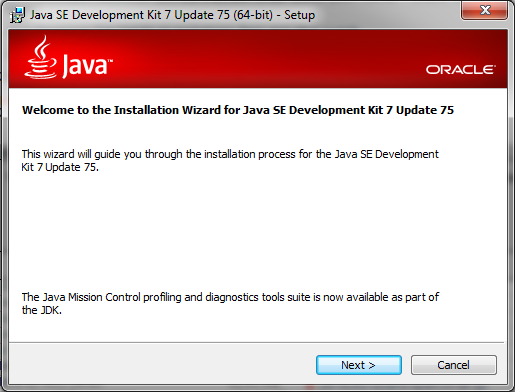
\includegraphics[width=0.45\textwidth]{imgs/jdk_2.png} & 
 				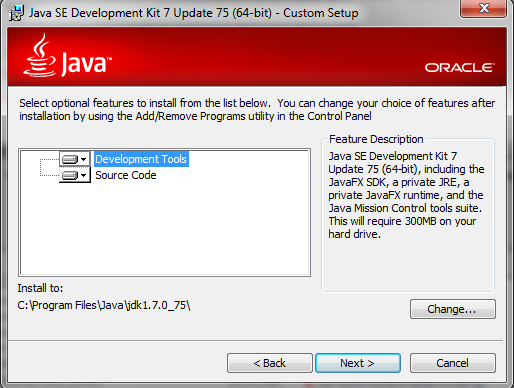
\includegraphics[width=0.45\textwidth]{imgs/jdk_3.png} \\
			\end{tabular}
            \caption{Instalaci�n del JDK, paso 1.}%
            \label{figImagen2}%
          \end{center}%
        \end{minipage}
      }%
    \end{center}%
  \end{figure}%
    \begin{figure}[]
    \begin{center}%
      \Ovalbox{%
        \begin{minipage}{\anchoFloat}%
          \begin{center}%
            \begin{tabular}{ l r}
 				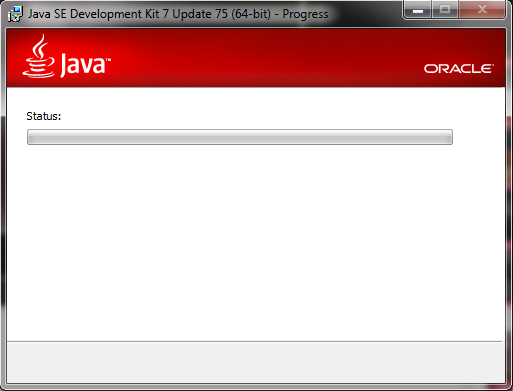
\includegraphics[width=0.45\textwidth]{imgs/jdk_4.png} & 
 				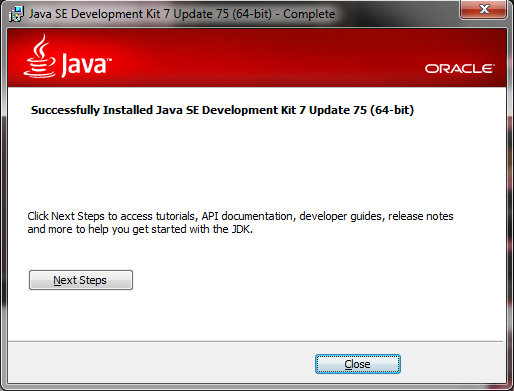
\includegraphics[width=0.45\textwidth]{imgs/jdk_5.png} \\
			\end{tabular}
            \caption{Instalaci�n del JDK, paso 2.}%
            \label{figImagen3}%
          \end{center}%
        \end{minipage}
      }%
    \end{center}%
  \end{figure}%
En la imagen \ref{figImagen2} vemos el primer paso para la instalaci�n del \textit{JDK}, el cual consta de dos pantallas. La primera ser� solamente una pantalla de bienvenida, por lo que debemos pulsar a \textit{next} o siguiente. La segunda pantalla nos muestra los elementos que van a ser instalados, esto no lo tocamos; adem�s nos muestra tambi�n el directorio en el que queremos instalar el \textit{JDK}, esto lo podemos dejar como est� o podemos, si queremos, configurarlo en un directorio personal que queramos. Lo �nico es que habr� que tener cuidado con el \textit{PATH} del equipo para que luego \textit{Android Studio} pueda encontrar la distribuci�n de \textit{JDK} que tengamos en nuestra m�quina.
\paragraph{}En la imagen \ref{figImagen3} nos encontramos el paso 2 para la instalaci�n de nuestro \textit{JDK}, este tambi�n consta de dos pantallas. La primera es el estado de la instalaci�n, veremos una barra que se ir� llenando en funci�n de que la instalaci�n vaya avanzando. Finalmente se nos mostrar� la pantalla que nos indicar� que la instalaci�n se ha realizado correctamente y nos da la opci�n de pulsar el bot�n \textit{Next Steps} uqe nos llevar� a la \textit{API de Java} o simplemente finalizar la instalaci�n.
\figura{1}{imgs/sdk_1.png}{P�gina de descarga de Android Studio}{figImagen4}{}\\
\section{Instalaci�n de Android Studio}
\paragraph{}Para la programaci�n del cliente se usar� \textit{Android Studio}, una herramienta ideada para programar en \textit{Android} exclusivamente. Lo primero que debemos hacer es dirigirnos a la p�gina web donde descargaremos Android Studio\footnote{\url{http://developer.android.com/sdk/index.html}}, la cual tendr� un aspecto similar al de la \ref{figImagen4}. En ella haremos \textit{click} sobre el bot�n de descarga (\textit{Download Android Studio}) y procederemos a la instalaci�n ejecutando el fichero que hemos descargado, todo este proceso es para un sistema operativo \textit{Windows}.
    \begin{figure}[]
    \begin{center}%
      \Ovalbox{%
        \begin{minipage}{\anchoFloat}%
          \begin{center}%
            \begin{tabular}{ l r}
 				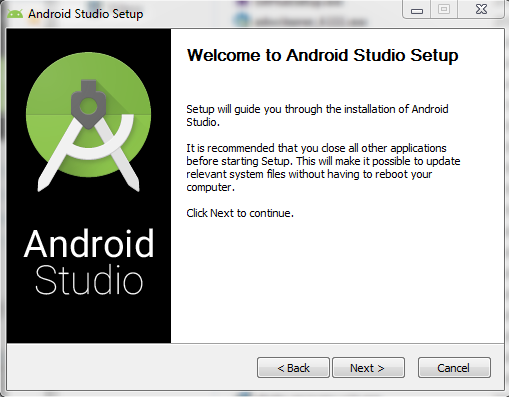
\includegraphics[width=0.45\textwidth]{imgs/sdk_2.png} & 
 				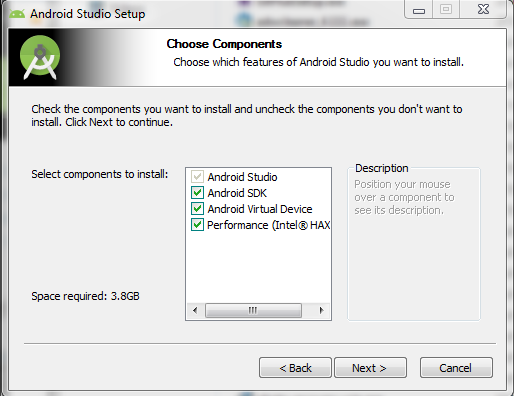
\includegraphics[width=0.45\textwidth]{imgs/sdk_3.png} \\
			\end{tabular}
            \caption{Instalaci�n de Android Studio, paso 1.}%
            \label{figImagen5}%
          \end{center}%
        \end{minipage}
      }%
    \end{center}%
  \end{figure}%
      \begin{figure}[]
    \begin{center}%
      \Ovalbox{%
        \begin{minipage}{\anchoFloat}%
          \begin{center}%
            \begin{tabular}{ l r}
 				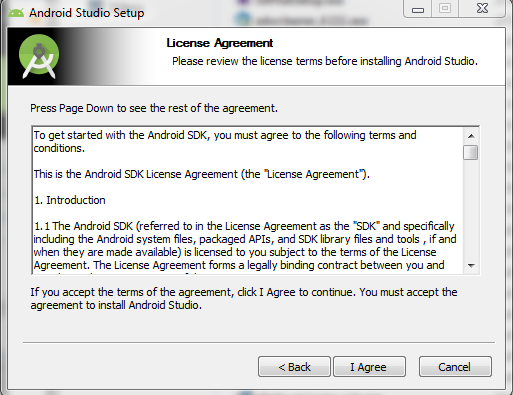
\includegraphics[width=0.45\textwidth]{imgs/sdk_4.png} & 
 				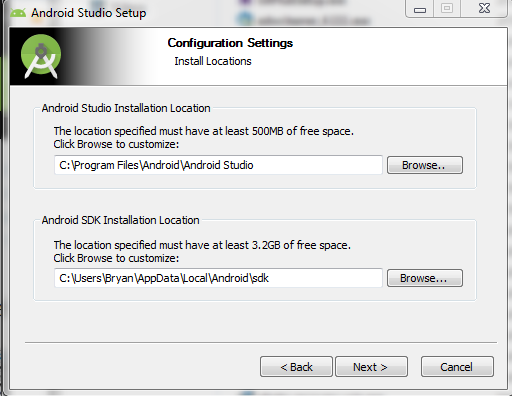
\includegraphics[width=0.45\textwidth]{imgs/sdk_5.png} \\
			\end{tabular}
            \caption{Instalaci�n de Android Studio, paso 2.}%
            \label{figImagen6}%
          \end{center}%
        \end{minipage}
      }%
    \end{center}%
  \end{figure}%
      \begin{figure}[]
    \begin{center}%
      \Ovalbox{%
        \begin{minipage}{\anchoFloat}%
          \begin{center}%
            \begin{tabular}{ l r}
 				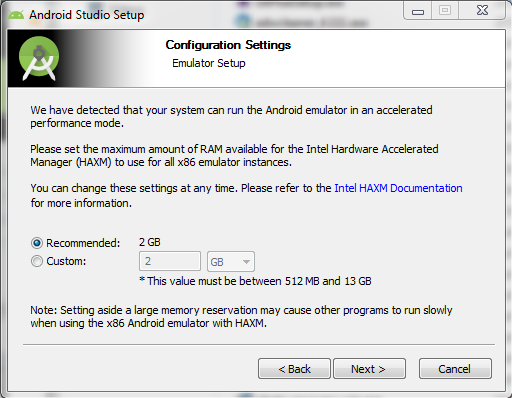
\includegraphics[width=0.45\textwidth]{imgs/sdk_6.png} & 
 				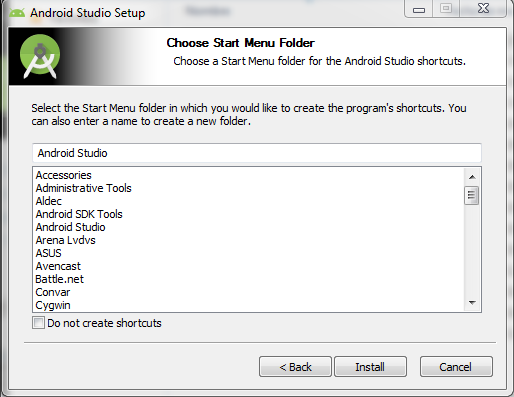
\includegraphics[width=0.45\textwidth]{imgs/sdk_7.png} \\
			\end{tabular}
            \caption{Instalaci�n de Android Studio, paso 3.}%
            \label{figImagen7}%
          \end{center}%
        \end{minipage}
      }%
    \end{center}%
  \end{figure}%
      \begin{figure}[]
    \begin{center}%
      \Ovalbox{%
        \begin{minipage}{\anchoFloat}%
          \begin{center}%
            \begin{tabular}{ l r}
 				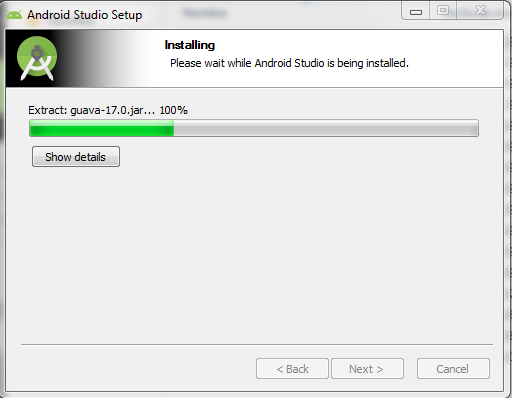
\includegraphics[width=0.45\textwidth]{imgs/sdk_8.png} & 
 				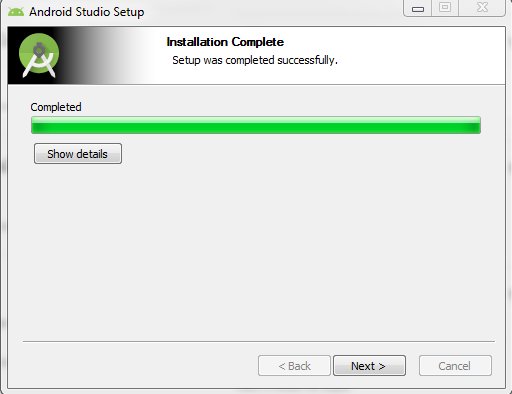
\includegraphics[width=0.45\textwidth]{imgs/sdk_9.png} \\
			\end{tabular}
            \caption{Instalaci�n de Android Studio, paso 4.}%
            \label{figImagen8}%
          \end{center}%
        \end{minipage}
      }%
    \end{center}%
  \end{figure}%
      \begin{figure}[]
    \begin{center}%
      \Ovalbox{%
        \begin{minipage}{\anchoFloat}%
          \begin{center}%
            \begin{tabular}{ l r}
 				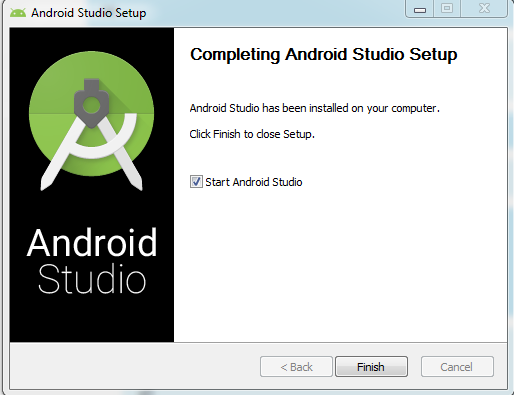
\includegraphics[width=0.45\textwidth]{imgs/sdk_10.png} & 
 				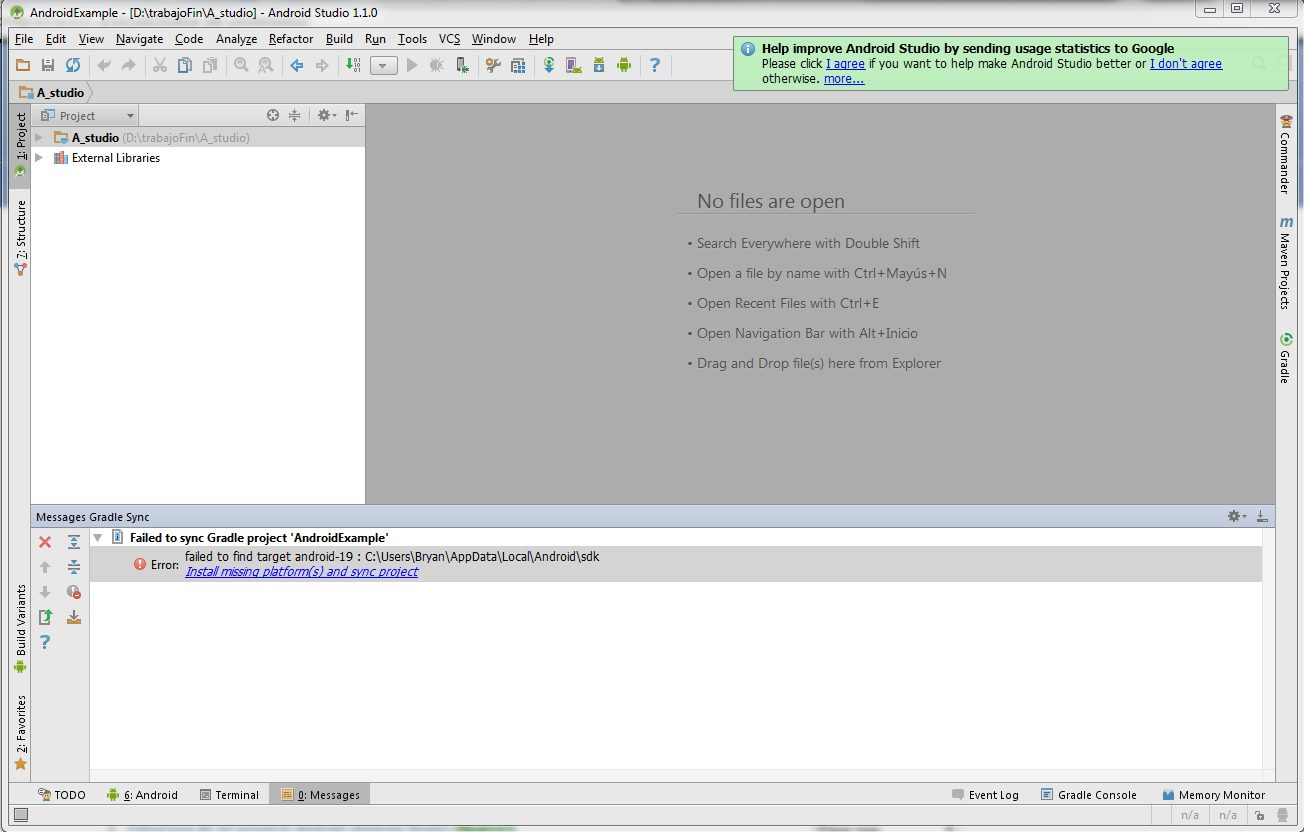
\includegraphics[width=0.45\textwidth]{imgs/sdk_11.png} \\
			\end{tabular}
            \caption{Instalaci�n de Android Studio, paso 5.}%
            \label{figImagen9}%
          \end{center}%
        \end{minipage}
      }%
    \end{center}%
  \end{figure}%
  
\paragraph{} En el primer paso de la instalaci�n, que se puede observar en la imagen \ref{figImagen5}, nos encontraremos con dos pantallas. La primera es simplemente una pantalla de bienvenida a la instalaci�n de nuestro \textit{Android Studio}, debemos pulsar al bot�n \textit{next} para empezar nuestra instalaci�n. Entonces pasamos a la siguiente pantalla y nos da la opci�n de elegir qu� elementos instalar, nosotros hemos dejado todos marcados pero puede que algunos no sean obligatoriamente necesarios. Una vez seleccionados los componentes de nuestra instalaci�n pasamos a dar el bot�n \textit{next} de la pantalla, entonces saltamos al paso 2.
\paragraph{}El segundo paso de nuestra instalaci�n lo podemos observar en la imagen \ref{figImagen6}. Una vez hemos pasado la selecci�n de componentes en nuestro \textit{Android Studio}, tenemos que aceptar la licencia del software, pasaremos a leer la licencia, si es de nuestro inter�s, y cuando estemos de acuerdo con ella, pulsaremos el bot�n \textit{I Agree}. Esto no habr� llevado a la siguiente pantalla de la instalaci�n, en la que podremos elegir los directorios en los que instalaremos nuestros componentes, nosotros los hemos dejado por defecto aunque se pueden personalizar en funci�n de las necesidades del usuario. Una vez establecida la configuraci�n de directorios en la instalaci�n, pulsaremos el bot�n \textit{next}.
\paragraph{}Pasaremos entonces al tercer paso de la instalaci�n, la cual puede ser vista en la imagen \ref{figImagen7}. En la primera pantalla de este paso tendremos que elegir la cantidad de memoria \textit{RAM} que asignaremos a nuestro \textit{Android Studio}, podemos dejar la cantidad recomendada o podemos asignarle m�s cantidad, si disponemos de ella, para que tenga un funcionamiento m�s fluido. Una vez establecido esto, se pulsara el bot�n \textit{next}. En nuestra segunda pantalla nos pregunta el directorio en el que se iniciar� la aplicaci�n y puedes poner la opci�n de no crear un acceso directo, nosotros hemos dejado la configuraci�n por defecto. Finalmente pulsamos el bot�n \textit{Install}.
\paragraph{}Ahora en el paso 4, el cual est� representado en la imagen \ref{figImagen8}, solamente tendremos que observar c�mo avanza la instalaci�n, esto se nos ir� mostrando a trav�s de una barra de progreso. Una vez se la barra se ha llenado podremos hacer \textit{click} en el bot�n \textit{Next} para pasar al �ltimo paso de nuestra instalaci�n.
\paragraph{}En nuestro quinto y �ltimo paso, el cual podemos ver en la imagen \ref{figImagen9}, se nos informar� de que la instalaci�n ha terminado y tendremos la opci�n de iniciar nuestro \textit{Android Studio} nada m�s acabar la instalaci�n. Entonces pulsamos al bot�n \textit{Finish}, se nos abrir� nuestro \textit{Android Studio} y con esto la instalaci�n se considera terminada.
\section{SDK Manager, instalando herramientas}
      \begin{figure}[]
    \begin{center}%
      \Ovalbox{%
        \begin{minipage}{\anchoFloat}%
          \begin{center}%
            \begin{tabular}{ l r}
 				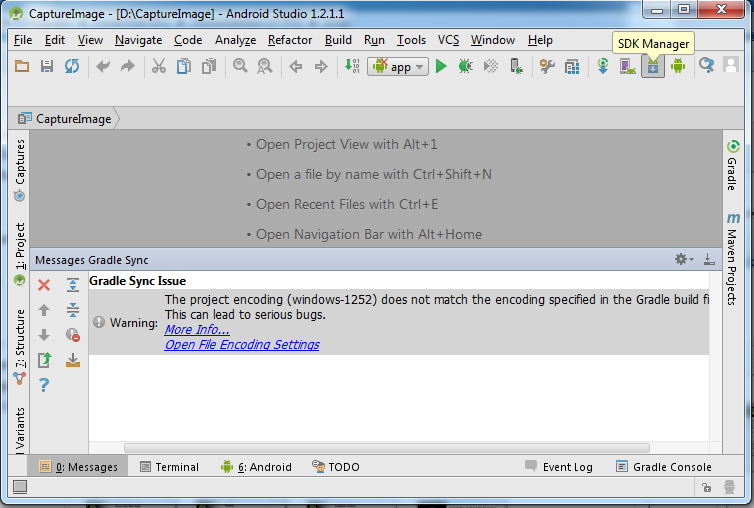
\includegraphics[width=0.45\textwidth]{imgs/mng1.png} & 
 				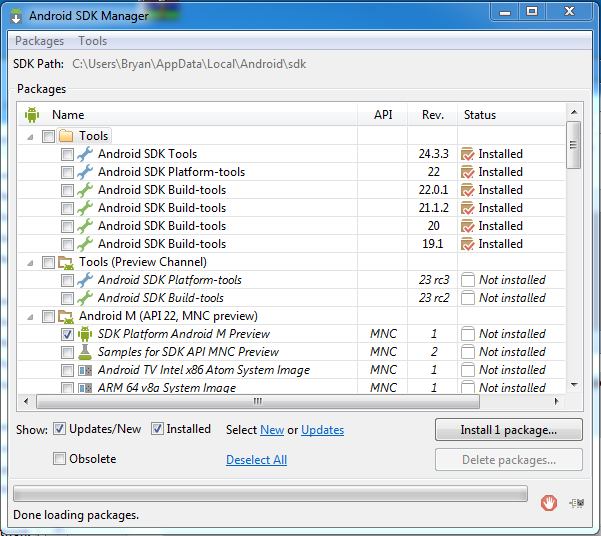
\includegraphics[width=0.45\textwidth]{imgs/mng2.png} \\
			\end{tabular}
            \caption{SDK Manager paso 1.}%
            \label{mng1}%
          \end{center}%
        \end{minipage}
      }%
    \end{center}%
  \end{figure}%
  \figura{1}{imgs/mng3.png}{SDK Manager paso 2.}{mng2}{}
Para que la futura importaci�n del proyecto se haga de manera correcta hay que instalar una serie de herramientas, estas pueden ser instaladas a trav�s del SDK \textit{Manager} del Android Studio. Para abrir el SDK \textit{Manager}, debemos hacer click sobre el bot�n resaltado en la primera imagen (\ref{mng1}). Seguidamente se nos abrir� una ventana gestora de paquetes de instalaci�n, que  se puede ver en la segunda imagen (\ref{mng1}). Entonces se seleccionan los paquetes a instalar, se abrir� una nueva ventana (\ref{mng2}) para aceptar las licencias, las aceptas y le das a instalar.

Los paquetes que necesitaremos ser�m:
\begin{itemize}
	\item Android SDK Tools
	\item Android SDK Platform-tools
	\item Android SDK Build-tools
	\item Todo el paquete Android 5.1.1(API 22)
	\item Android Support Repository
	\item Android Support Library
	\item Google Repository
	\item Google USB Driver
	\item Google Web Driver
\end{itemize}
\section{Importando Cliente en Android Studio}
\figura{1}{imgs/Import1.png}{Importando proyecto en Android Studio}{import1}{}
\figura{1}{imgs/Import2.png}{Importando proyecto en Android Studio}{import2}{}
\figura{0.60}{imgs/Import3.png}{Importando proyecto en Android Studio}{import3}{}
\figura{1}{imgs/Import4.png}{Importando proyecto en Android Studio}{import4}{}
Se procede a explicar la manera de importar el proyecto en Android Studio, que es la aplicaci�n con la que se ha trabajado y con la que mejor se puede trabajar sobre el proyecto. Primero deberemos iniciar el Android Studio (\ref{import1}), seguidamente le damos a \textit{File} o Archivo -> \textit{Open\dots } o Abrir\dots (\ref{import2}). Entonces se nos abrir� una ventana (\ref{import3}) en la que deberemos navegar hasta la carpeta en la que tenemos almacenado el proyecto, seleccionamos el archivo con nombre Imagen y que tiene el icono de Android Studio. Entonces le damos a aceptar y el programa proceder� a importar el s�lo todo el proyecto (\ref{import4}), al finalizar podremos ponernos enseguida a trabajar.

\section{Instalaci�n de Matlab}
\label{MATLAB}
Para poder ejecutar el \textit{script} de instalaci�n del servidor, el cu�l se instala en Ubuntu, debemos tener como pre-instalado Matlab. Para ello necesitaremos una licencia, en este proyecto se ha trabajado con la licencia de estudiante de la UBU.

Al trabajar en Ubuntu de 64 bit, hemos descargado el instalador para Linux de Matlab. Hay que recordar que Caffe s�lo trabaja con ciertas versiones de Matlab a la hora de descargar el instalador (2014a/b, 2013a/b, and 2012b). Una vez se ha descargado el instalador se tiene que ejecutar el archivo\textit{install} del conjunto de archivos que hemos descargado (\ref{lst:install}).
\begin{lstlisting}[frame=none,language=bash,caption={Ejecutando \textit{install} de Matlab},basicstyle=\large,label={lst:install}]
sudo ./install
\end{lstlisting}
Entonces nos aparecer� una ventana a trav�s de la cual guiaremos nuestra instalaci�n.

Describiremos la instalaci�n con el tipo de licencia que se ha usado en el proyecto.

Primero debemos elegir la primera opci�n de la primera imagen y despu�s aceptar la licencia de la segunda imagen en el paso 1 (\ref{mat1}). 

Seguidamente, en el segundo paso de instalaci�n. deberemos aportar nuestras credenciales, nuestra cuenta de MathWorks, como se muestra en la primera imagen y despu�s seleccionar el lugar de instalaci�n, tal y como se muestra en la segunda imagen del paso 2 (\ref{mat2}). Se recomienda dejar la carpeta de destino de la instalaci�n a la que viene por defecto, porque evitar� futuros problemas de configuraci�n cuando instalemos el servidor y sus dependencias.

En el tercer paso de la instalaci�n decidiremos si creamos un link para invocar a Matlab desde el terminal, esto se recomienda hacerlo y dejar el link en la ruta por defecto del instalador, como podemos ver en la primera imagen. Despu�s se nos pedir� seleccionar los paquetes que queremos instalar a Matlab, seleccionaremos los b�sicos, como se ve en la imagen dos del tercer paso (\ref{mat3}).

En el cuarto paso se nos pide la confirmaci�n de los paquetes que hemos solicitado instalar en el paso previo, esto puede verse en la primera imagen; comprobaremos que tenemos los paquetes que deseamos y le damos a confirmar. En la segunda imagen vemos la barra de progreso de la instalaci�n que se nos muestra mientras Matlab es instalado (\ref{mat4}).

En el quinto y �ltimo paso se te muestra la ventana de instalaci�n satisfactoria y te comunica que debes activar Matlab para poder usarlo. Dejamos la opci�n de ``Activar MATLAB'' marcada y le damos a siguiente. As� concluimos la instalaci�n de Matlab, pero se tiene que activar antes (\ref{mat5}).

  \begin{figure}[]
    \begin{center}%
      \Ovalbox{%
        \begin{minipage}{\anchoFloat}%
          \begin{center}%
            \begin{tabular}{ l r}
 				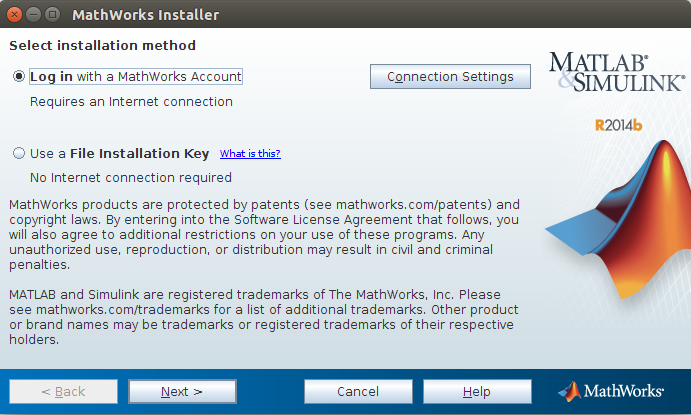
\includegraphics[width=0.45\textwidth]{imgs/matlab1.png} & 
 				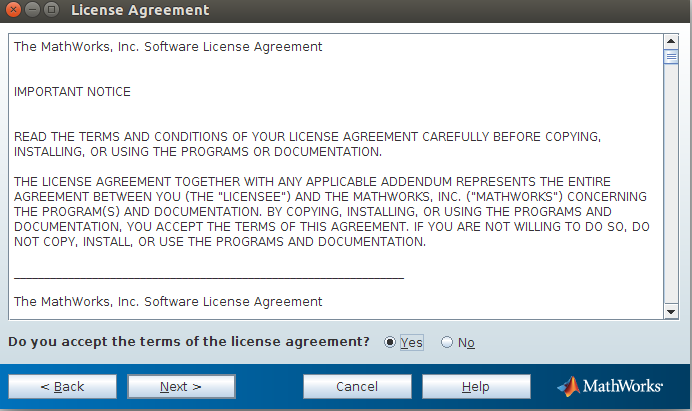
\includegraphics[width=0.45\textwidth]{imgs/matlab2.png} \\
			\end{tabular}
            \caption{Instalaci�n de Matlab paso 1.}%
            \label{mat1}%
          \end{center}%
        \end{minipage}
      }%
    \end{center}%
  \end{figure}%
  \begin{figure}[]
    \begin{center}%
      \Ovalbox{%
        \begin{minipage}{\anchoFloat}%
          \begin{center}%
            \begin{tabular}{ l r}
 				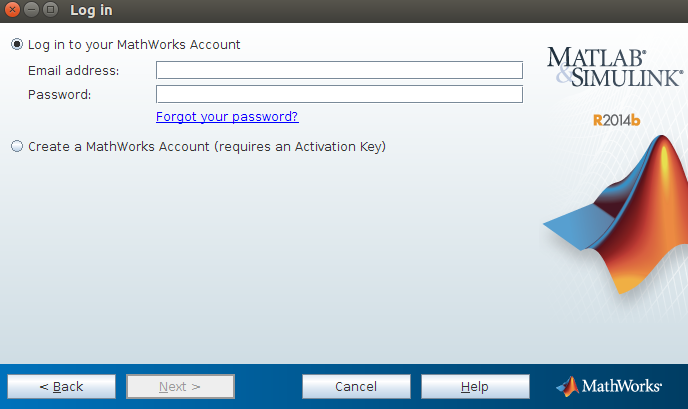
\includegraphics[width=0.45\textwidth]{imgs/matlab3.png} & 
 				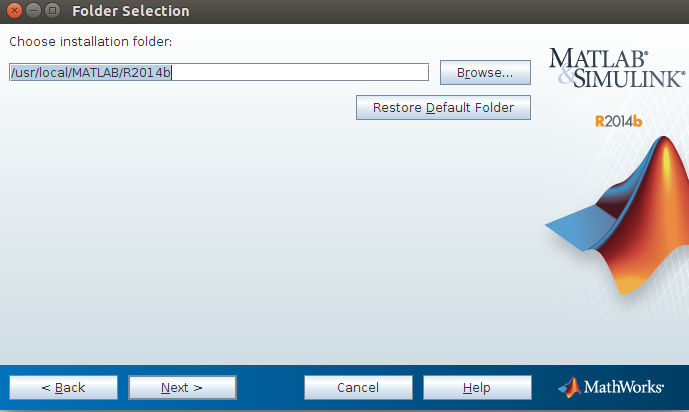
\includegraphics[width=0.45\textwidth]{imgs/matlab4.png} \\
			\end{tabular}
            \caption{Instalaci�n de Matlab paso 2.}%
            \label{mat2}%
          \end{center}%
        \end{minipage}
      }%
    \end{center}%
  \end{figure}%
  \begin{figure}[]
    \begin{center}%
      \Ovalbox{%
        \begin{minipage}{\anchoFloat}%
          \begin{center}%
            \begin{tabular}{ l r}
 				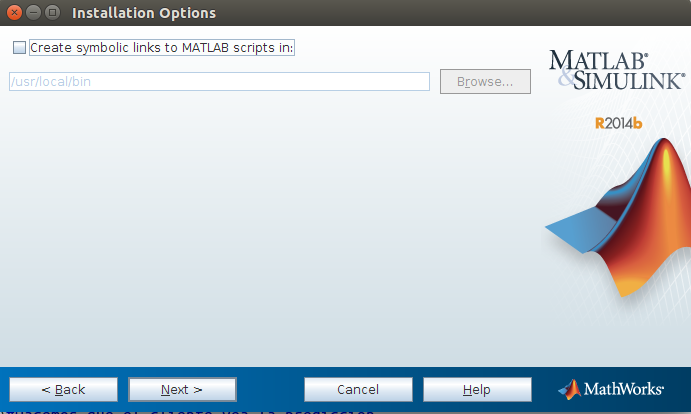
\includegraphics[width=0.45\textwidth]{imgs/matlab5.png} & 
 				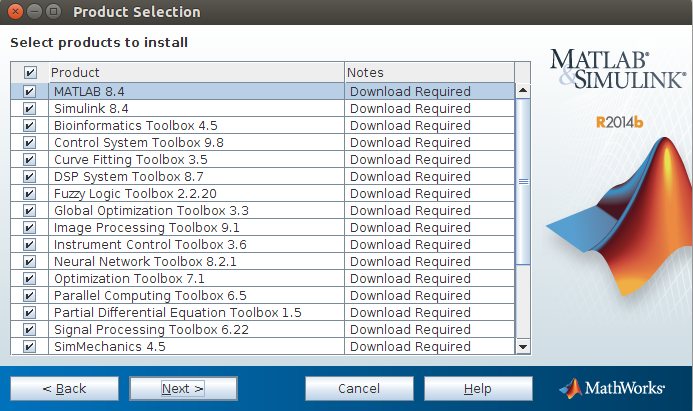
\includegraphics[width=0.45\textwidth]{imgs/matlab6.png} \\
			\end{tabular}
            \caption{Instalaci�n de Matlab paso 3.}%
            \label{mat3}%
          \end{center}%
        \end{minipage}
      }%
    \end{center}%
  \end{figure}%
  \begin{figure}[]
    \begin{center}%
      \Ovalbox{%
        \begin{minipage}{\anchoFloat}%
          \begin{center}%
            \begin{tabular}{ l r}
 				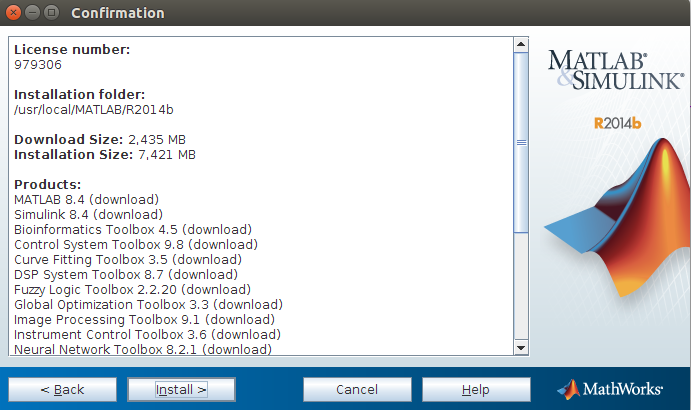
\includegraphics[width=0.45\textwidth]{imgs/matlab7.png} & 
 				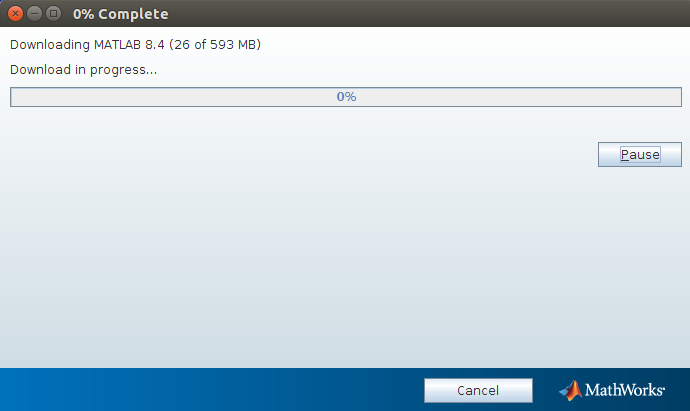
\includegraphics[width=0.45\textwidth]{imgs/matlab8.png} \\
			\end{tabular}
            \caption{Instalaci�n de Matlab paso 4.}%
            \label{mat4}%
          \end{center}%
        \end{minipage}
      }%
    \end{center}%
  \end{figure}%
 \figura{1}{imgs/matlab9.png}{Instalaci�n de Matlab paso 5}{mat5}{}
 \subsection{Activar MATLAB}
 \label{ActMATLAB}
  \begin{figure}[]
    \begin{center}%
      \Ovalbox{%
        \begin{minipage}{\anchoFloat}%
          \begin{center}%
            \begin{tabular}{ l r}
 				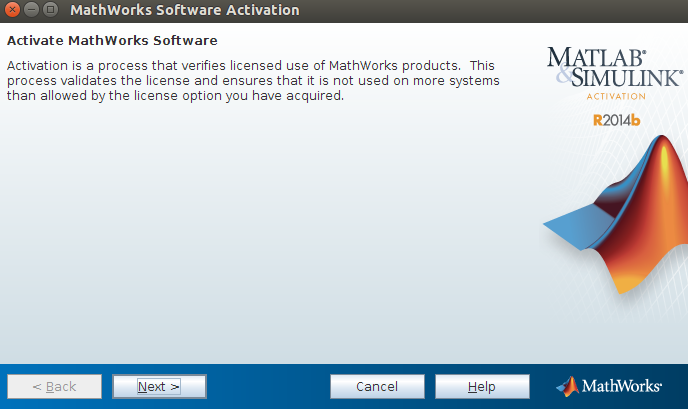
\includegraphics[width=0.45\textwidth]{imgs/Activation1.png} & 
 				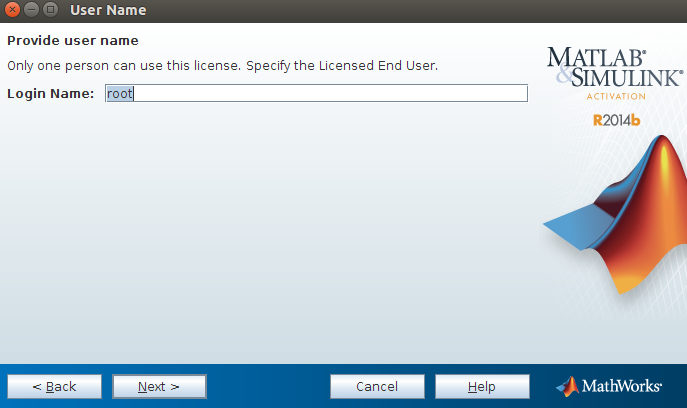
\includegraphics[width=0.45\textwidth]{imgs/Activation2.png} \\
			\end{tabular}
            \caption{Activaci�n de Matlab paso 1.}%
            \label{act1}%
          \end{center}%
        \end{minipage}
      }%
    \end{center}%
  \end{figure}%
  \begin{figure}[]
    \begin{center}%
      \Ovalbox{%
        \begin{minipage}{\anchoFloat}%
          \begin{center}%
            \begin{tabular}{ l r}
 				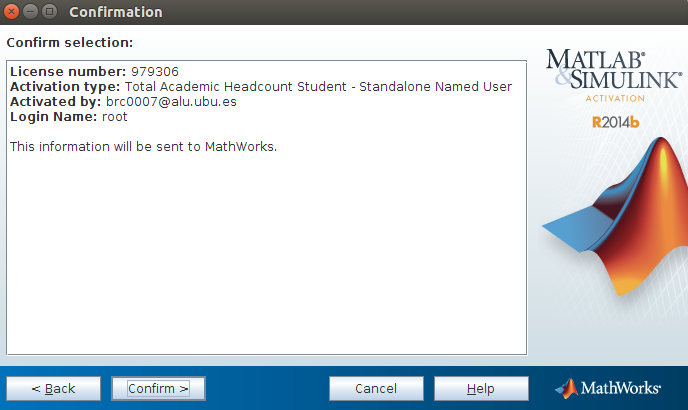
\includegraphics[width=0.45\textwidth]{imgs/Activation3.png} & 
 				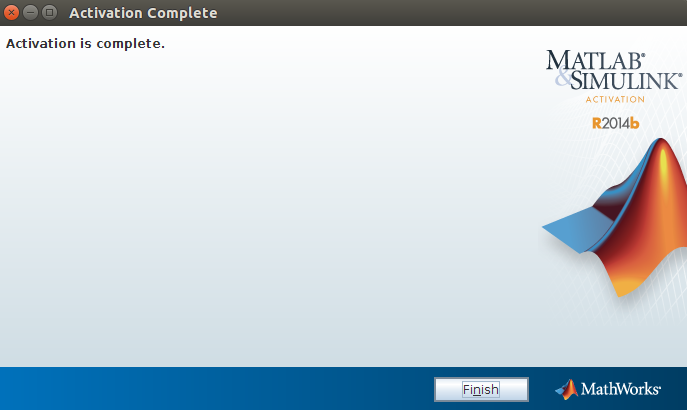
\includegraphics[width=0.45\textwidth]{imgs/ActivationF.png} \\
			\end{tabular}
            \caption{Activaci�n de Matlab paso 2.}%
            \label{act2}%
          \end{center}%
        \end{minipage}
      }%
    \end{center}%
  \end{figure}%
Despu�s de la instalaci�n de Matlab se debe haber recibido la solicitud de activaci�n del mismo, por lo que se nos abre una ventana de activaci�n como se puede ver en la primera imagen del paso 1(\ref{act1}). Esta ventana es s�lo informativa, por lo que daremos al bot�n de siguiente. En la segunda imagen del paso 1 podemos ver que nos pide el nombre de usuario con el que se va a querer activar Matlab, se aconseja poner el nombre de usuario normal, no root. Una vez decidido el nombre con el que se va a activar Matlab se pulsa al bot�n de siguiente.

En el transcurso del primer paso hasta el segundo paso, el activador habr� hecho algunas comprobaciones con nuestra licencia y nos muestra una ventana de confirmaci�n, comprobamos que los datos son correctos y pulsamos el bot�n confirmar, esto se puede ver en la primera imagen del paso 2 (\ref{act2}). Final mente nos muestra una ventana informativa explicando que la activaci�n ha sido un �xito, como vemos en la segunda imagen del paso 2.
\section{Instalaci�n de CUDA}
\label{CUDA}
Si no nos encontramos en una m�quina virtual y queremos instalar los \textit{drivers} de NVIDIA en nuestra m�quina junto con CUDA, entonces tenemos que seguir unos pasos especiales para hacerlos, los cu�les ser�n explicados en este apartado para el caso de querer instalar controladores de NVIDIA, de lo contrario, s�lo se tendr� que descomentar las siguientes l�neas del \textit{script} de instalaci�n del servidor y sus dependencias:
\begin{lstlisting}[frame=none,language=bash,caption={Instalaci�n de CUDA en \textit{script}},basicstyle=\large,label={lst:install}]
sudo apt-get install curl
cd ~/Downloads/
curl -O "http://developer.download.nvidia.com/compute/cuda/6_5/rel/installers/cuda_6.5.14_linux_64.run"
chmod +x cuda_6.5.14_linux_64.run
./cuda_6.5.14_linux_64.run --kernel-source-path=/usr/src/linux-headers-`uname -r`/
\end{lstlisting}

En caso de querer instalar los controladores de NVIDIA, entonces tendremos que proceder a realizar una operaci�n m�s compleja para realizar su instalaci�n, debido a que para instalar los controladores no debemos estar en modo interfaz gr�fica y tener desactivadas ciertos servicios.

Primero tendremos que desinstalar cualquier rastro de alg�n controlador de NVIDIA que tengamos previamente en nuestra m�quina, lo hacemos con el siguiente comando:
\begin{lstlisting}[frame=none,language=sh,caption={Instalaci�n \textit{driver} de NVIDIA paso 1},basicstyle=\large]
sudo apt-get remove --purge nvidia* 
\end{lstlisting}
Despu�s de esto se deber� desactivar el controlador libre ``noveau'', el cual lo desactivamos de la siguiente manera:
\begin{itemize}
	 \item Primero, se tiene que ejecutar el siguiente comando en tu shell:
	 \begin{lstlisting}[frame=none,language=sh,caption={Instalaci�n \textit{driver} de NVIDIA paso 2},basicstyle=\large]
	 sudo nano /etc/modprobe.d/blacklist.conf
	 \end{lstlisting}
	 \item Segundo, debes a�adir lo siguiente al final del fichero, que se ha abierto tras ejecutar el anterior comando, y guardar los cambios:
	 \begin{lstlisting}[frame=none,language=sh,caption={Instalaci�n \textit{driver} de NVIDIA paso 3},basicstyle=\large]
	 blacklist nouveau
	 \end{lstlisting}
	 \item Tercero, una vez realizado esto tienes que ejecutar los siguientes comando para que los cambios hagan efecto, aunque si no lo hacen tendr�s que reiniciar el ordenador:
	 \begin{lstlisting}[frame=none,language=sh,caption={Instalaci�n \textit{driver} de NVIDIA paso 4},basicstyle=\large]
	 echo options nouveau modeset=0 | sudo tee -a /etc/modprobe.d/nouveau-kms.conf
	 update-initramfs -u
	 \end{lstlisting}
\end{itemize}

Ahora que se ha desactivado el controlador libre ``noveau'', procedemos a la instalaci�n del \textit{driver}, pero este debe ser sin interfaz gr�fica. Para trabajar sin interfaz gr�fica, primero, debemos pulsar la secuencia de teclas: CTRL+ALT+F1. Esto iniciar� un shell sin interfaz gr�fica.

Antes que nada debemos identificarnos ante el sistema, para identificarnos deberemos introducir nuestro nombre de usuario y la contrase�a, la contrase�a se te solicitar� una vez hayas introducido el nombre de usuario.

Una vez en el shell se procede a detener el demonio, controlador interno de Unix, que se encarga de mantener en ejecuci�n la interfaz gr�fica, para ello tenemos que ejecutar la siguiente orden en el shell:
\begin{lstlisting}[frame=none,language=sh,caption={Instalaci�n \textit{driver} de NVIDIA paso 5},basicstyle=\large]
sudo service gdm stop
\end{lstlisting}
Ahora se procede a descargar el \textit{driver} con la secuencia que antes hemos comentado sobre el \textit{script} de instalaci�n:
\begin{lstlisting}[frame=none,language=bash,caption={Instalaci�n \textit{driver} de NVIDIA paso 6},basicstyle=\large,label={lst:install}]
sudo apt-get install curl
cd ~/Downloads/
curl -O "http://developer.download.nvidia.com/compute/cuda/6_5/rel/installers/cuda_6.5.14_linux_64.run"
chmod +x cuda_6.5.14_linux_64.run
./cuda_6.5.14_linux_64.run --kernel-source-path=/usr/src/linux-headers-`uname -r`/
\end{lstlisting}
Una vez ejecutado esto, se iniciar� la instalaci�n y deber�s aceptar la licencia e instalar todo lo que se te propone, los controladores NVIDIA, CUDA y los ejemplos, todos deben ser instalados en sus directorios por defecto.

Cuando esto haya terminado tendr�s ya instalado los \textit{drivers} de NVIDIA, pero a�n queda hacer un par de pasos, lanzar el demonio de la interfaz de nuevo y reiniciar el sistema, hazlo con los siguientes comandos:
\begin{lstlisting}[frame=none,language=bash,caption={Instalaci�n \textit{driver} de NVIDIA paso 7},basicstyle=\large,label={lst:install}]
sudo service gdm start
sudo reboot
\end{lstlisting}

Con esto ya tendremos el controlador de NVIDIA y CUDA instalados, siendo CUDA necesario para la instalaci�n de las dependencias del servidor y las herramientas.
\section{Instalando Servidor y sus Dependencias}
Para instalar el servidor se ha usado en parte una peque�a gu�a\footnote{\url{https://github.com/BVLC/caffe/wiki/Ubuntu-14.04-VirtualBox-VM}}. Gracias a esta gu�a se instal� correctamente las dependencias, a la que podr�s acceder mirando la bibliograf�a\cite{Wiki}.

Para usar el \textit{script} de instalaci�n deber�s haber seguido los dos anteriores pasos (\ref{CUDA}) (\ref{MATLAB}). Ahora para iniciar el proceso de instalaci�n deber�s ejecutar el siguiente comando en el \textit{shell}:
\begin{lstlisting}[frame=none,language=bash,caption={Instalar Servidor},basicstyle=\large,label={lst:installS}]
sudo . ./install.sh
\end{lstlisting}

\textbf{IMPORTANTE:} Si te encuentras en una m�quina virtual, deber�s ir al \textit{script} de instalaci�n y modificarlo \textbf{antes de ejecutar la instalaci�n}. Deber�s cambiar la linea 47 de la siguiente manera:
\begin{lstlisting}[frame=none,language=bash,caption={Cambio para m�quinas virtuales},basicstyle=\large,label={lst:vm}]
#Esta es la l�nea original en el script:
cp ~/Proyecto-Fin-de-Grado/servidor/Install/Makefile.config ~/caffe

#Esto es lo que se debe poner:
cp ~/Proyecto-Fin-de-Grado/servidor/Install/MaquinaVirtual/Makefile.config ~/caffe
\end{lstlisting}

Si tienes alg�n problema con la instalaci�n o con el \textit{script}, se procede a explicar paso a paso qu� hace el programa de instalaci�n y qu� deber�as hacer t� para instalarlo sin el uso del \textit{script}. Todo esto debe ser siempre realizado tras haber hecho los anteriores dos pasos (\ref{CUDA}) (\ref{MATLAB}).

En primer lugar se va a un directorio por defecto para hacer la instalaci�n y seguidamente se instala la herramienta ``git'' para clonar los proyectos desde Github.
\begin{lstlisting}[frame=none,language=bash,caption={Explicaci�n Instalaci�n 1},basicstyle=\large,label={lst:exp1}]
cd ~
apt-get install git
\end{lstlisting}
Vemos que hemos hecho la acci�n de irnos a un directorio por defecto, este directorio sera la base de toda la instalaci�n y, por tanto, no se recomienda cambiarlo para que la configuraci�n del servidor sea m�s sencilla.

Ahora se procede a instalar los paquetes esenciales de Linux, adem�s de actualizar las cabeceras del \textit{kernel} a su �ltima versi�n para evitar errores futuros.
\begin{lstlisting}[frame=none,language=bash,caption={Explicaci�n Instalaci�n 2},basicstyle=\large,label={lst:exp2}]
apt-get install build-essential
apt-get install linux-headers-`uname -r`
\end{lstlisting}
En este paso clonaremos nuestro proyecto al directorio principal de instalaci�n.
\begin{lstlisting}[frame=none,language=bash,caption={Explicaci�n Instalaci�n 3},basicstyle=\large,label={lst:exp3}]
cd ~
git clone https://github.com/garfio1/Proyecto-Fin-de-Grado.git
\end{lstlisting}

En el siguiente paso se ha copiado la l�nea de instalaci�n de dependencias de la Wiki\cite{Wiki} de Github para instalar Caffe. Esto instalar� todas las dependencias necesarias para Caffe.
\begin{lstlisting}[frame=none,language=bash,caption={Explicaci�n Instalaci�n 4},basicstyle=\large,label={lst:exp4}]
apt-get install -y libprotobuf-dev libleveldb-dev libsnappy-dev libopencv-dev libboost-all-dev libhdf5-serial-dev protobuf-compiler gfortran libjpeg62 libfreeimage-dev libatlas-base-dev git python-dev python-pip libgoogle-glog-dev libbz2-dev libxml2-dev libxslt-dev libffi-dev libssl-dev libgflags-dev liblmdb-dev python-yaml
easy_install pillow
\end{lstlisting}

Ahora se procede a clonar Caffe\cite{jia2014caffe} en nuestro directorio principal de instalaci�n.
\begin{lstlisting}[frame=none,language=bash,caption={Explicaci�n Instalaci�n 5},basicstyle=\large,label={lst:exp5}]
cd ~
git clone https://github.com/BVLC/caffe.git
\end{lstlisting}

Ahora se instalan todos los requisitos para poder instalar PyCaffe, esto no deber�a ser necesario porque no usamos PyCaffe, pero la evoluci�n del proyecto NeuralTalk apunta a que acabar� usando esta librer�a de Caffe para Python, as� que se instala aqu� tambi�n para tener trabajo ya hecho.
\begin{lstlisting}[frame=none,language=bash,caption={Explicaci�n Instalaci�n 5},basicstyle=\large,label={lst:exp5}]
cd caffe
cat python/requirements.txt | xargs -L 1 sudo pip install
\end{lstlisting}

Ahora se procede a hacer unos enlaces con los nombres de las librer�as Python para que PyCaffe funcione de manera adecuada y correcta.

\begin{lstlisting}[frame=none,language=bash,caption={Explicaci�n Instalaci�n 6},basicstyle=\large,label={lst:exp6}]
sudo ln -s /usr/include/python2.7/ /usr/local/include/python2.7
sudo ln -s /usr/local/lib/python2.7/dist-packages/numpy/core/include/numpy/ /usr/local/include/python2.7/numpy
\end{lstlisting}

En el siguiente paso el programa de instalaci�n supone que has seguido todos los pasos hasta ahora como se han ido comentando y sustituye el Makefile.config de Caffe por el que viene en el proyecto. Puesto que si has instalado las cosas seg�n se han ido comentando, este archivo deber�a servirte para poder hacer los \textit{make} (instalaci�n a trav�s de un Makefile) de Caffe.
\begin{lstlisting}[frame=none,language=bash,caption={Explicaci�n Instalaci�n 7},basicstyle=\large,label={lst:exp7}]
rm ~/caffe/Makefile.config
cp ~/Proyecto-Fin-de-Grado/servidor/Install/Makefile.config ~/caffe
\end{lstlisting}

Finalmente se ejecuta la instalaci�n de Caffe a trav�s de la herramienta make, se instalan tanto MatCaffe como PyCaffe.
\begin{lstlisting}[frame=none,language=bash,caption={Explicaci�n Instalaci�n 8},basicstyle=\large,label={lst:exp8}]
make pycaffe
make matcaffe
make all
make test
\end{lstlisting}

En este punto nos falta el clonado del proyecto NeuralTalk en nuestra m�quina, por tanto, es lo que se procede a hacer en el pen�ltimo paso de la instalaci�n
\begin{lstlisting}[frame=none,language=bash,caption={Explicaci�n Instalaci�n 9},basicstyle=\large,label={lst:exp9}]
cd ~
git clone https://github.com/karpathy/neuraltalk.git
\end{lstlisting}

Finalmente nos resta �nicamente instalar las librer�as espec�ficas usadas en el servidor para pasar a la configuraci�n del proyecto para que funcione de manera adecuada.
\begin{lstlisting}[frame=none,language=bash,caption={Explicaci�n Instalaci�n 10},basicstyle=\large,label={lst:exp10}]
pip install beautifulsoup
pip install flask
\end{lstlisting}

Con esto tenemos instalado en nuestra m�quina todas las herramientas necesarias para el funcionamiento del servidor. Ahora hay que pasar a la configuraci�n  del mismo. Como se ha explicado en el apartado de Aspectos Relevantes (\ref{chap:AspectosRelevantes}), la configuraci�n no ha sido nada sencilla; pero se ha preparado para que ahora sea mucho m�s sencilla y r�pida.
\section{Configuraci�n del Servidor}
En este paso se proceder� a explicar c�mo se configura el servidor para que funcione, ahora resulta una tarea bastante sencilla porque se han preparado una serie de variables y ficheros para que esto sea as�.

En primer lugar, y lo m�s importante, es tener claro el directorio principal de la instalaci�n, pues todas las herramientas deber�an estar instaladas en �l. Si se ha seguido correctamente los pasos y se h mantenido el mismo directorio principal de instalaci�n, deber�as ser capaz de obtenerlo con la siguiente secuencia de comandos:
\begin{lstlisting}[frame=none,language=bash,caption={Configurando el servidor 1},basicstyle=\large,label={lst:conf1}]
cd ~
pwd
\end{lstlisting}
\figura{1}{imgs/Paso1.png}{Comprobando directorio principal de instalaci�n}{dirPrin}{}
El resultante de ejecutar los anteriores comandos es una cadena de caracteres que te comunican cu�l es el directorio principal de la instalaci�n, por ejemplo a mi me devuelve ``/home/bryan'', como se puede ver en la imagen \ref{dirPrin}.

Antes de continuar con la instalaci�n, debemos cambiar los permisos de las carpetas NeuralTalk y Proyecto-Fin-de-Grado para poder hacer la configuraci�n sobre ellas,  esto se hace de la siguiente manera:
lugar ejecutaremos el siguiente comando para empezar con la configuraci�n:
\begin{lstlisting}[frame=none,language=bash,caption={Configurando el servidor 2},basicstyle=\large,label={lst:conf2}]
chmod -R 777 ~/Proyecto-Fin-de-Grado
chmod -R 777 ~/neuraltalk
\end{lstlisting}

Una vez se ha detectado este directorio, podemos empezar con la configuraci�n del servidor. En primer lugar ejecutaremos el siguiente comando para empezar con la configuraci�n:
\begin{lstlisting}[frame=none,language=bash,caption={Configurando el servidor 3},basicstyle=\large,label={lst:conf3}]
cd ~/Proyecto-Fin-de-Grado/servidor
\end{lstlisting}
Con el anterior comando nos situamos en la carpeta en la que tendremos el primer documento a modificar. Tendremos que abrir con un editor de texto el archivo ``serv.py'' que nos encontramos en dicha carpeta. Podemos hacerlo con el siguiente comando si queremos, aunque el procesador de texto es a elecci�n del usuario:
\begin{lstlisting}[frame=none,language=bash,caption={Configurando el servidor 4},basicstyle=\large,label={lst:conf4}]
vi serv.py
\end{lstlisting}
Una vez tengamos abierto el archivo, deberemos localizar dos l�neas en concreto. Las l�neas a localizar con en las que se define la ruta del directorio principal de instalaci�n y en la que se define el usuario definido en la licencia de MATLAB. Podemos ver las l�neas a continuaci�n:
\begin{lstlisting}[frame=none,language=Python,caption={Configurando el servidor 5},basicstyle=\large,label={lst:conf5}]
#Deber�an estar en las l�neas 12 y 24 respectivamente pero si no lo est�n s�lo busca lo siguiente:
ROOT='/home/bryan'

USER='bryan'
\end{lstlisting}
Una vez hemos localizado las l�neas anteriores, en la constante ``ROOT'' deber�s poner el directorio que obtuviste en \ref{lst:conf1} o tu directorio principal de instalaci�n, el c�digo est� preparado para que, si has instalado las herramientas en el directorio correcto, no tengas que modificar m�s variables ni que estar picando el c�digo en busca de problemas; y en la constante ``USER'', deber�s poner el nombre de usuario que utilizaste al realizar el paso de Activaci�n de MATLAB(\ref{ActMATLAB}). Con estas modificaciones ya hemos configurado la mitad del servidor, s�lo nos queda ahora hacer las modificaciones pertinentes para que la herramienta NeuralTalk funcione en nuestra m�quina.

Para empezar, junto con el proyecto se facilita una copia del archivo ``extract\_ features.m'' de NeuralTalk, s�lo que este archivo est� modificado para que la configuraci�n se muy sencilla. Lo que haremos ser� borrar el archivo que viene por defecto junto con la herramienta NeuralTalk y se copiar� el que viene adjunto con el proyecto, lo haremos de la siguiente manera:
\begin{lstlisting}[frame=none,language=bash,caption={Configurando el servidor 6},basicstyle=\large,label={lst:conf6}]
rm ~/neuraltalk/matlab_features_reference/extract_features.m
cp ~/Proyecto-Fin-de-Grado/servidor/Install/extract_features.m ~/neuraltalk/matlab_features_reference/
\end{lstlisting}

Ahora debemos dirigirnos a la carpeta en la que acabamos de copiar el fichero y abrirlo para proceder a modificarlo, esto se puede hacer v�a comandos de shell o puede el usuario abrirlo con cualquier procesador de texto que el prefiera:
\begin{lstlisting}[frame=none,language=bash,caption={Configurando el servidor 7},basicstyle=\large,label={lst:conf7}]
cd ~/neuraltalk/matlab_features_reference/
vi extract_features.m
\end{lstlisting}

Una vez tenemos el fichero abierto para su modificaci�n debemos buscar una l�nea si estamos en una m�quina anfitriona, dos si estamos en una m�quina virtual:
\begin{lstlisting}[frame=none,language=Matlab,caption={Configurando el servidor 8},basicstyle=\large,label={lst:conf8}]
%Si estamos en m�quina virtual buscamos tambi�n la siguiente l�nea, t�picamente est� en la l�nea 3:
use_gpu = 1;

%Deber�a estar en la l�nea 5
root='/home/bryan';
\end{lstlisting}

Si nos encontramos en una m�quina virtual, la variable ``use\_ gpu''  deber�amos ponerla con el valor  0. Mientras que lo siguiente se hace tanto para m�quina virtual como para m�quina anfitriona, se cambiar� la variable ``root'' por el directorio que se obtuvo en \ref{lst:conf1}.

Con esto ya tenemos hecho las modificaciones pertinentes para que el servidor funcione correctamente, s�lo nos queda descargar un fichero necesario para la ejecuci�n del \textit{script} de MATLAB. El fichero en cuesti�n ser� descargado de la siguiente manera:
\begin{lstlisting}[frame=none,language=Matlab,caption={Configurando el servidor 9},basicstyle=\large,label={lst:conf9}]
cd ~/Proyecto-Fin-de-Grado/servidor/uploads
wget "http://www.robots.ox.ac.uk/~vgg/software/very_deep/caffe/VGG_ILSVRC_16_layers.caffemodel"
\end{lstlisting}

Ahora ya podemos ejecutar el servidor, para ello podremos ejecutar los siguientes comandos:
\begin{lstlisting}[frame=none,language=Matlab,caption={Ejecutando el servidor},basicstyle=\large,label={lst:ex}]
cd ~/Proyecto-Fin-de-Grado/servidor
sudo python serv.py
\end{lstlisting}

Ahora hay que tener en cuenta que, si has realizado la instalaci�n sobre una m�quina anfitriona, podr�a darse un error al ejecutar el servidor, este error mostrar� un mensaje al ejecutar Matlab, que ser� el siguiente:
\begin{lstlisting}[frame=none,language=Matlab,caption={Error en CUDA},basicstyle=\large,label={lst:as}]
Cannot open shared object file: No such file or directory
\end{lstlisting}
Para resolver este error solamente debemos ejecutar el siguiente comando:
\begin{lstlisting}[frame=none,language=bash,caption={Soluci�n al error de CUDA},basicstyle=\large,label={lst:se}]
sudo ldconfig /usr/local/cuda/lib64
\end{lstlisting}

Como punto final cabe destacar que este tutorial de instalaci�n funciona para las herramientas en la versi�n en la que se encontraban al realizar el proyecto, estas podr�n ser encontradas en el CD entregado por si este tutorial no funcionara con las versiones actuales.
%
%\portadasAuxiliares{Anexo V - Manual del usuario}
%\chapter{Manual del usuario}
%\section{Introducci�n}
En este anexo se presentar� el manual de usuario, d�nde se explicar� c�mo instalar y usar la aplicaci�n.
\subsection{Instalar Aplicaci�n}
Si queremos extraer la aplicaci�n del proyecto, deberemos dirigirnos al directorio <</Proyecto-Fin-de-Grado/Imagen/app>>, en �l encontraremos un archivo llamado \cmd{app-release.apk}, este archivo se guardar� en el dispositivo en el que se vaya a instalar la aplicaci�n.
\begin{figure}[]
    \begin{center}%
      \Ovalbox{%
        \begin{minipage}{\anchoFloat}%
          \begin{center}%
            \begin{tabular}{ l r}
 				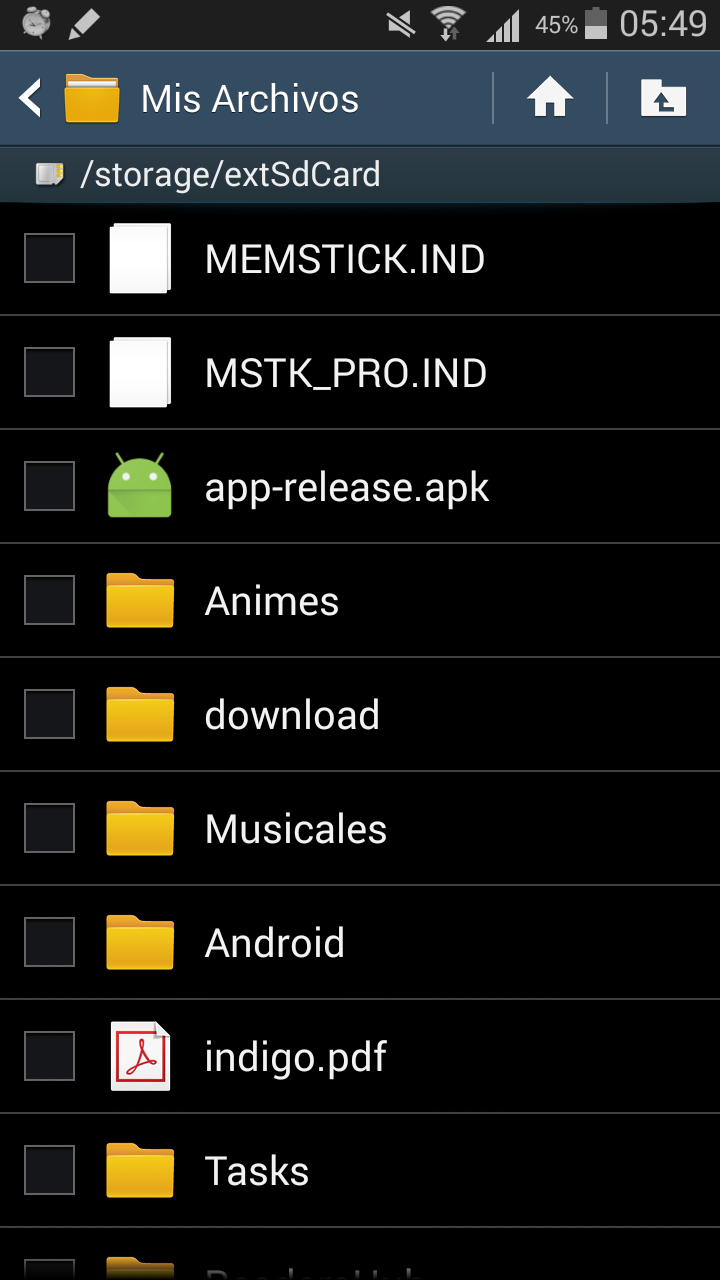
\includegraphics[width=0.30\textwidth]{imgs/us1.png} & 
 				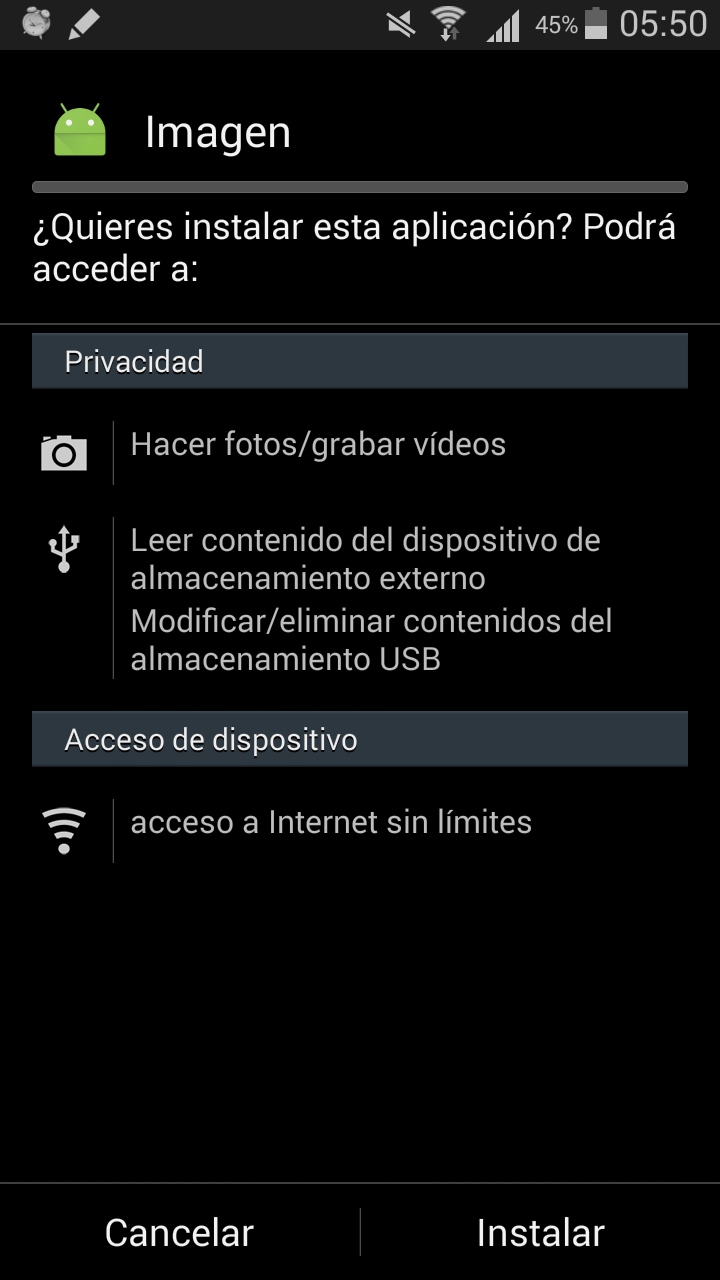
\includegraphics[width=0.30\textwidth]{imgs/us2.png} \\
			\end{tabular}
            \caption{Instalando aplicaci�n paso 1.}%
            \label{app1}%
          \end{center}%
        \end{minipage}
      }%
    \end{center}%
  \end{figure}%
  \begin{figure}[]
    \begin{center}%
      \Ovalbox{%
        \begin{minipage}{\anchoFloat}%
          \begin{center}%
            \begin{tabular}{ l r}
 				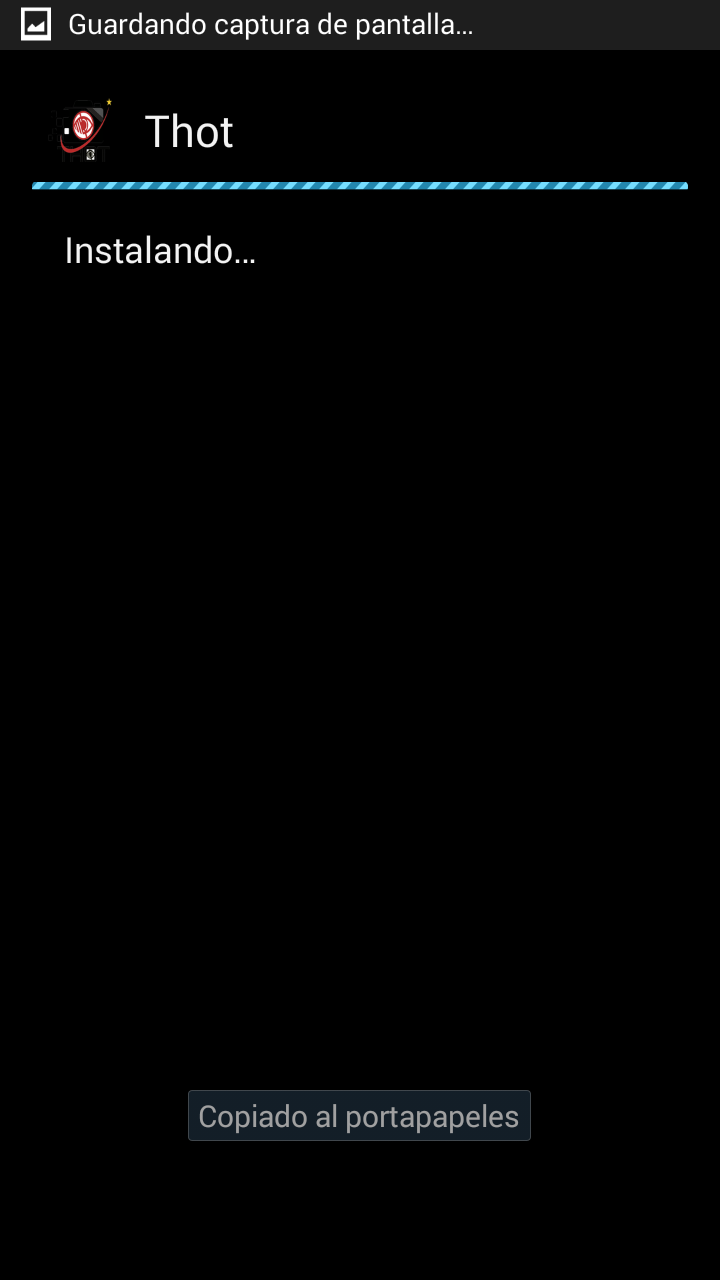
\includegraphics[width=0.30\textwidth]{imgs/us3.png} & 
 				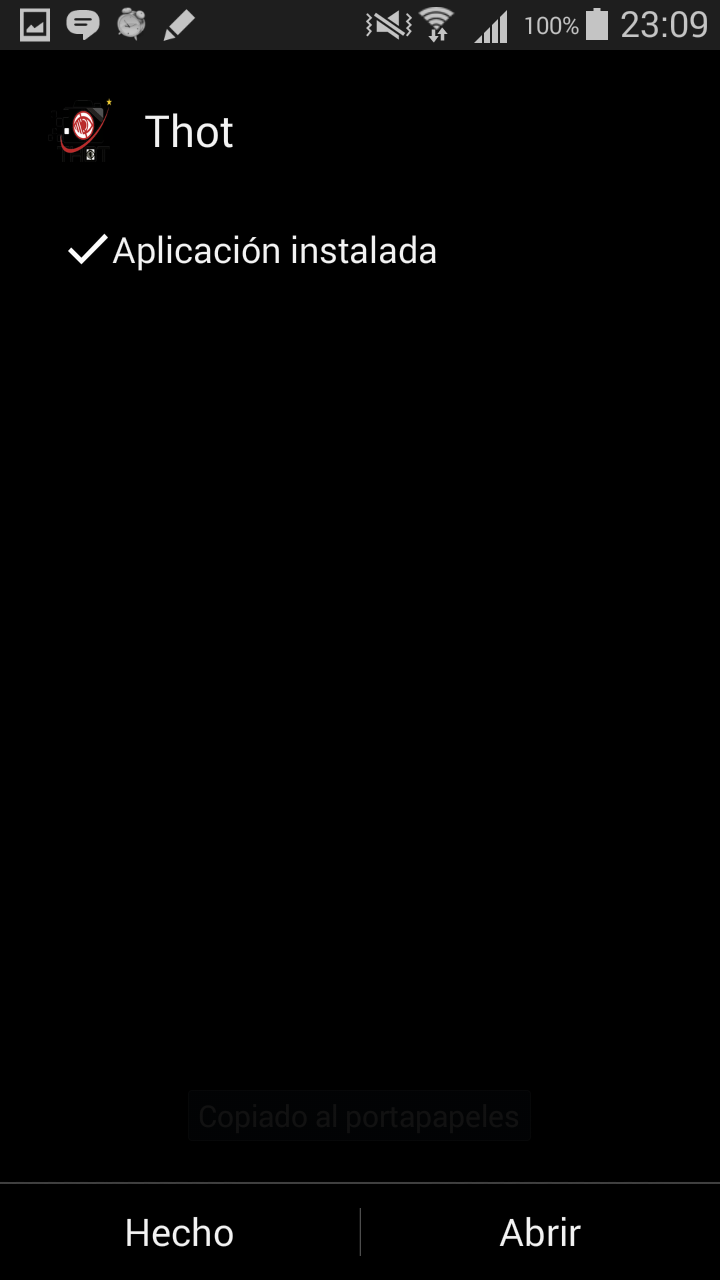
\includegraphics[width=0.30\textwidth]{imgs/us4.png} \\
			\end{tabular}
            \caption{Instalando aplicaci�n paso 2.}%
            \label{app2}%
          \end{center}%
        \end{minipage}
      }%
    \end{center}%
  \end{figure}%
  \figura{0.45}{imgs/us5.png}{Instalando aplicaci�n paso 3}{app3}{}
  Hay que destacar que la instalaci�n de la aplicaci�n se debe hacer de forma manual, a�n no se ha planificado ni modelado una manera de que una persona invidente pueda hacerlo, por tanto esta deber� tener alguien que le ayude a instalarla.
  
  Para empezar la instalaci�n, tenemos que buscar en los archivos del dispositivo el fichero de instalaci�n con el nombre \cmd{app-release.apk}, una vez encontrado tocamos la pantalla sobre este y se abrir� una ventana de instalaci�n. En la ventana de instalaci�n se nos muestra los permisos que requiere la aplicaci�n y nos da la opci�n de instalar, presionamos al bot�n de instalar para proceder con la instalaci�n. Estos pasos est�n representados en la imagen \ref{ver Figura app1}.
  
  Despu�s de haber presionado el bot�n de instalar, se nos muestra una ventana que nos informa de que la aplicaci�n se est� instalando. Seguidamente, una vez se ha instalado la aplicaci�n, se mostrar� una ventana inform�ndonos de que la aplicaci�n se ha instalado correctamente y nos dar� la opci�n de abrirla.Esto esta representado en la imagen \ref{ver Figura app2}.
  
  Si hemos abierto la aplicaci�n, se nos mostrar� la pantalla inicial (ver Figura \ref{app3}).

\section{Uso de la aplicaci�n}
Cuando se ha iniciado la aplicaci�n, y se nos muestra la pantalla inicial (ver Figura \ref{app3}), el usuario deber� apuntar con el m�vil en la direcci�n que se quiera tomar la foto y tocar la pantalla. Entonces la aplicaci�n se encargar� de mandar la foto y recibir la predicci�n.

Si el usuario no sabe qu� tiene que hacer cuando abre la aplicaci�n, pasado un tiempo, se le lee un mensaje en voz alta con la librer�a \textit{Text to Speech} dici�ndole qu� tiene que hacer.

Tras la ejecuci�n de la petici�n al servidor y el procesado de la imagen, la aplicaci�n leer� en voz alta la predicci�n. Y aqu� termina la ejecuci�n de la aplicaci�n, si se quiere hacer otra predicci�n, se debe esperar a que la aplicaci�n indique que podemos tomar otra foto.


%
% AP�NDICES
%\backmatter
%\appendix

% A�adir entrada en el �ndice: Ap�ndices
%\addcontentsline{toc}{chapter}{Ap�ndices}
%
%\portadasAuxiliares{Ap�ndice A - Gu�a r�pida de Version One}
%\chapter{Gu�a r�pida de Version One}
%\input{apendiceA}
%
%\portadasAuxiliares{Ap�ndice B - Licencia GNU GPL}
%\chapter{Licencia GNU GPL}
%\input{apendiceB}

%
%Bibliograf�a
\normalem
\bibliografia{referencias}


% Otras referencias
%\bibliografiaOtras{otrasreferencias}

\end{document}
